% latexmk -pdf -bibtex main

\documentclass[a4paper, 11pt]{report}

%% Language and font encodings
\usepackage[english]{babel}
\usepackage[utf8x]{inputenc}
\usepackage[T1]{fontenc}

%% Sets page size and margins
\usepackage[a4paper,top=2cm,bottom=2cm,left=3cm,right=3cm,marginparwidth=1.75cm]{geometry}

%% Useful packages
\usepackage{amsmath}
\usepackage{amssymb}
\usepackage{graphicx}
\usepackage[colorinlistoftodos]{todonotes}
\usepackage[colorlinks=true, allcolors=blue]{hyperref}
\usepackage[numbers]{natbib}
\usepackage{algpseudocode}
\usepackage{algorithm}
\usepackage{eurosym}
\usepackage[breakall]{truncate}
\usepackage{chngpage}
\usepackage{listings}
\usepackage{xcolor}
\usepackage{caption}
\usepackage{subcaption}
\usepackage{multirow}
\usepackage{multicol}
\usepackage{setspace}
\usepackage{enumitem}

%New colors defined below
\definecolor{codegreen}{rgb}{0,0.6,0}
\definecolor{codegray}{rgb}{0.5,0.5,0.5}
\definecolor{codepurple}{rgb}{0.58,0,0.82}
\definecolor{backcolour}{rgb}{0.95,0.95,0.92}

%Code listing style named "mystyle"
\lstdefinestyle{mystyle}{
  backgroundcolor=\color{backcolour}, commentstyle=\color{codegreen},
  keywordstyle=\color{magenta},
  numberstyle=\tiny\color{codegray},
  stringstyle=\color{codepurple},
  basicstyle=\ttfamily\footnotesize,
  breakatwhitespace=false,         
  breaklines=true,                 
  captionpos=b,                    
  keepspaces=true,                 
  numbers=left,                    
  numbersep=5pt,                  
  showspaces=false,                
  showstringspaces=false,
  showtabs=false,                  
  tabsize=2
}

%"mystyle" code listing set
\lstset{style=mystyle}

\newtheorem{theorem}{Theorem}
\title{An Empirical Analysis of Mean Reversion Strategies for Pairs Trading in Decentralised Exchanges}
\author{Devam Savjani}
% Update supervisor and other title stuff in title/title.tex

\begin{document}
\begin{titlepage}

\newcommand{\HRule}{\rule{\linewidth}{0.5mm}} % Defines a new command for the horizontal lines, change thickness here

%----------------------------------------------------------------------------------------
%	LOGO SECTION
%----------------------------------------------------------------------------------------


\includegraphics[width=8cm]{title/logo.eps}\\[1cm] % Include a department/university logo - this will require the graphicx package
 
%----------------------------------------------------------------------------------------

\center % Center everything on the page

%----------------------------------------------------------------------------------------
%	HEADING SECTIONS
%----------------------------------------------------------------------------------------

\textsc{\LARGE MEng Individual Project}\\[1.5cm] % Name of your university/college
\textsc{\Large Imperial College London}\\[0.5cm] % Major heading such as course name
\textsc{\large Department of Computing}\\[0.5cm] % Minor heading such as course title

%----------------------------------------------------------------------------------------
%	TITLE SECTION
%----------------------------------------------------------------------------------------
\makeatletter
\HRule \\[0.4cm]
{ \huge \bfseries \@title}\\[0.4cm] % Title of your document
\HRule \\[1.5cm]
 
%----------------------------------------------------------------------------------------
%	AUTHOR SECTION
%----------------------------------------------------------------------------------------

\begin{minipage}{0.4\textwidth}
\begin{flushleft} \large
\emph{Author:}\\
\@author % Your name
\end{flushleft}
\end{minipage}
~
\begin{minipage}{0.4\textwidth}
\begin{flushright} \large
\emph{Supervisor:} \\
Prof. Thomas Lancaster \\[1.2em] % Supervisor's Name
\emph{Second Marker:} \\
Unknown % second marker's name
\end{flushright}
\end{minipage}\\[2cm]
\makeatother

% If you don't want a supervisor, uncomment the two lines below and remove the section above
%\Large \emph{Author:}\\
%John \textsc{Smith}\\[3cm] % Your name

%----------------------------------------------------------------------------------------
%	DATE SECTION
%----------------------------------------------------------------------------------------

{\large \today}\\[2cm] % Date, change the \today to a set date if you want to be precise

\vfill % Fill the rest of the page with whitespace

\end{titlepage}

\begin{abstract}
    SOME ABSTRACT
\end{abstract}

\renewcommand{\abstractname}{Acknowledgements}
\begin{abstract}
My sincere gratitude goes to my supervisor Dr. Thomas E. Lancaster and second marker Mr. Ivan Procaccini for their advice and guidance throughout the project.
\\[5mm]
I would also send my gratitude to my family and friends whose motivation helped me throughout this degree.
\end{abstract}

\tableofcontents
% \listoffigures
% \listoftables

\chapter{Introduction}
\section{Motivation}
Since the advent of Bitcoin, the groundbreaking peer-to-peer payment network and cryptocurrency, the blockchain technology ecosystem has witnessed an exponential surge, propelling the emergence of numerous cryptocurrencies that are now widely utilised and traded. The soaring volatility of cryptocurrencies has not only captured the attention of retail investors, with some reaping substantial returns while others suffered significant losses~\cite{losing_money_on_crypto_2021}. Moreover, prominent financial institutions have joined the fray, aiming to capitalise on this novel tradable asset~\cite{gondek_what_nodate}. Consequently, this surge of interest has spurred the development of more sophisticated approaches to cryptocurrency trading.
\\[3mm]
Initially, trading cryptocurrencies posed a significant challenge for individuals lacking technical expertise, with the first recorded transaction occurring on $12^{th}$ October 2009 via a PayPal transaction~\cite{noauthor_history_nodate}. However, the landscape has since evolved, giving rise to various centralised and decentralised cryptocurrency exchanges. Centralised exchanges have gained popularity, offering a user-friendly interface allowing investors with limited technical knowledge to access the ecosystem. In contrast, decentralised exchanges (DEXes) operate on blockchain networks and facilitate direct peer-to-peer transactions using smart contracts. The prevalence of centralised exchanges is evident, as depicted in Figure \ref{fig:dex_to_cex}, where the proportion of trades on DEXes remained minimal until the summer of 2020 but has steadily increased.
\vspace{-.2cm}
\begin{figure}[htb!]
    \centering
    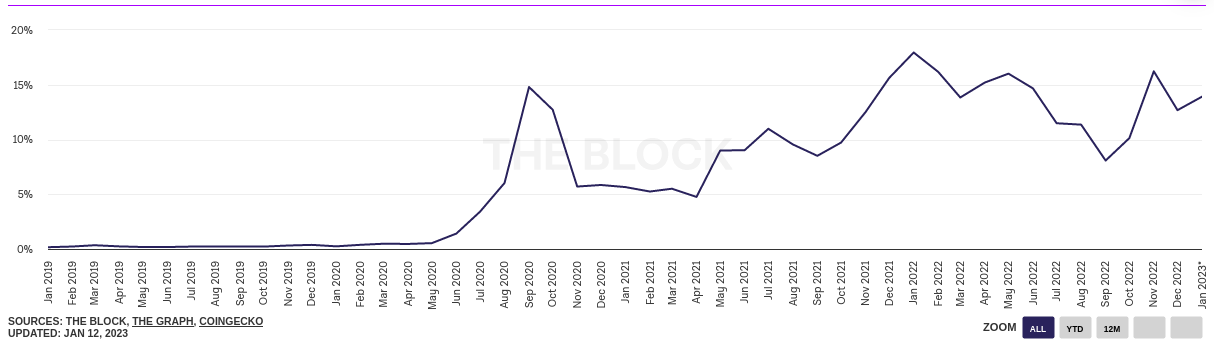
\includegraphics[width=\textwidth]{introduction/Images/dex_to_cex.png}
    \caption{{DEX} to {CEX} {Spot} {Trade} {Volume}~\cite{dex_to_cex}}
    \label{fig:dex_to_cex}
\end{figure}
\vspace{-1cm}
\section{Objectives}
This poses a question about whether advanced trading strategies can exploit arbitrage opportunities on decentralised exchanges. Surprisingly, existing research on cryptocurrency arbitrage has solely focused on triangular and cyclic arbitrage. Therefore, this project aims to be the first to explore the potential profitability of employing mean reversion techniques in cryptocurrency pairs trading on decentralised exchanges. By implementing diverse variations of the mean reversion strategy, the project aims to unravel the most effective methods for achieving remarkable profits.

\section{Contributions}
The work presented in the report is motivated by the rise in trading activity on decentralised exchanges. Exploring statistical arbitrage techniques on DEXes provides an opportunity to gain insights into decentralised markets' unique dynamics and potential profitability. The contributions are as follows:
\begin{enumerate}[wide, labelwidth=!, labelindent=2ex]
    \itemsep-0.1em
    \item \textbf{Analysis of Liquidity Pool Pairs} - The analysis of liquidity pool pairs involves examining the correlation and cointegration between different liquidity pools. This analysis provides insights into the pricing dynamics and long-term inter-pool relationships, exposing potential arbitrage opportunities. 
    \item \textbf{Backtesting System} - A meticulous backtesting system was developed to replicate the execution of trades by utilising comprehensive historical data directly sourced from the Ethereum blockchain. This system enabled the evaluation of trading strategies under realistic and reliable market conditions, allowing for a thorough assessment of their performance.
    \item \textbf{Live Trading System} - To facilitate real-time trading and interaction with the Ethereum blockchain, a dynamic live trading system was designed and implemented. This system enabled the seamless execution of trading strategies in a live market environment.
    \item \textbf{Trading Strategies} - The mean reversion strategy relies on the hedge ratio, a key parameter that impacts the strategy's risk exposure and trading volumes. To assess the performance of different hedge ratio estimation methods, multiple strategies were employed: constant hedge ratio using ordinary least squares (OLS) as a benchmark, sliding window using OLS, lagged using OLS, Granger Causality test-based OLS model, and Kalman Filter-based hedge ratio estimation.
    \item \textbf{Novel Analysis of Applying Mean Reversion on Decentralised Exchanges}~- The analysis showed that the Kalman Filter strategy outperformed other mean reversion strategies and current research, achieving an Annual Percentage Return of 81.14\%. Equally noteworthy, the Granger Causality and Lagged strategies delivered substantial returns of 48.85\% and 38.70\%, respectively, surpassing returns observed in prior research on mean reversion and pure arbitrage across diverse asset classes.
\end{enumerate}

\section{Ethical Issues}

The ethics of cryptocurrencies are widely debated for reasons such as anonymity, leading it to be the choice of currency used by criminals and illegal institutions, volatility and lack of regulation. The high volatility makes cryptocurrencies and decentralised finance very risky for retail investors that do not have the technical or financial know-how making investing in cryptocurrencies.
\\[3mm]
Another aspect of cryptocurrencies that has raised ethical questions is the energy consumption and carbon dioxide emission from the mining of cryptocurrencies. Formal research has also found that `approximately 69 million metric tons of CO2 (Carbon dioxide) emission due to bitcoin mining'~\cite{egiyi2020cryptocurrency}. Thus, this is an ethical concern that was considered when designing the strategies so that the number of transactions that do not result in a profit, i.e. do not add value to the project, is limited.
\\[3mm]
In addition to the concerns above, although this project aims to find riskless profits, \textit{`free lunches'}, it is not, in any form, of financial advice. Those who use the research or software used in the development and research process to attempt to get favourable results, are liable for the losses or gains. 

\chapter{Background}

\section{Cryptocurrencies}
Before going delving into the financial side of the project, it is important to understand the underlying assets and the technology that drive them.

\subsection{Blockchain}
The building blocks of cryptocurrencies comes from blockchain. Blockchain is a distributed ledger that stores data, in blocks, in a chain, comprising the data itself as well has a full transaction history~\cite{nofer2017blockchain}. Below shows a diagram of blocks in a blockchain.

\begin{figure}[!htb]
    \centering
    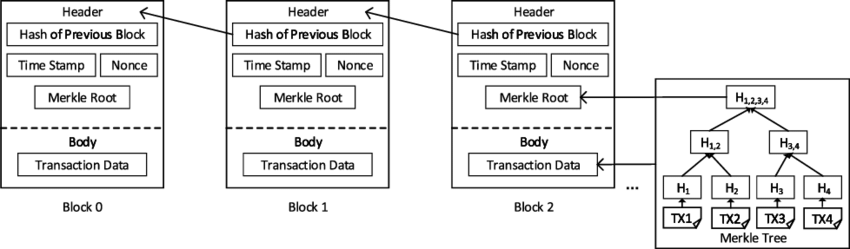
\includegraphics[width=0.8\textwidth]{background/Images/The-structure-of-a-Blockchain.png}
    \caption{Blockchain Diagram~\cite{inbookBlockchain}}
\end{figure}

\subsubsection{Header, Hash of Previous Block and Timestamp}
The timestamp and hashes of the block and its' predecessing block are all used to ensure the ordering of blocks within a chain. By hashing the data to a fixed size, and storing in its succeeding block makes the tampering of chains difficult as it would mean the chain deviates from its old state. In addition to this, by hashing and using Nonce, blockchain employs the Proof-of-Work algorithm to ensure correctness. The Proof-of-Work algorithm is used to confirm and add new transaction to the chain.

\subsubsection{Nonce}
A nonce, `Number Only used Once', is a number that is added to a hashed block to make the transaction more secure. It is randomly generated which miners use to validate a transaction. A miner first guesses a nonce, appends the guess to the hash of the current header. The miner then rehashes the value and compares this to the target hash. If the guess was correct, the miner is granted the block~\cite{noauthor_components_2021}.

\subsubsection{Merkle root}
A merkle root is also stored in each block to validate transactions in an efficient manner, in terms of storage and searching. A merkle tree is a a tree of hashes where each leaf node is it's data hash and it's parent node, the hash of their children's hashes. In storing the merkle root, we do not need to directly store each transaction in each block, and also allows a quick search for any malicious alterations in differing blocks~\cite{noauthor_merkle_nodate}.

\subsection{Ethereum}
One of the first application of blockchain was by Satoshi Nakamoto to create the first `purely peer-to-peer version of electronic cash'~\cite{nakamoto2009bitcoin}. Nakamoto's solution details the process in which a decentralised, peer to peer approach to verify and track transactions without a centralized institution. Since then, many other technologies derived from using blockchain as its underlying technology. One of them was proposed by Vitalik Buterin, the co-founder of Ethereum, in a whitepaper that proposed the idea of using smart contracts to create financial products and services that could operate independently of traditional financial institutions, hence decentralised finance was birthed~\cite{buterin2014next}.

\subsubsection{Ethereum}
Ethereum's architecture is similar to bitcoin's but has a few differences, one of which is the blockchain contains a copy of the transaction list and the most recent state. The process of how transactions are validated is below:
\begin{enumerate}
    \itemsep0em
    \item Validate the parent block
    \item Validate that the current timestamp is greater that the previous timestamp
    \item Check that the Ethereum concepts are valid
    \item Perform Proof of Stake on the block
    \item Check for errors and gas
    \item Validate the final state
\end{enumerate}

\noindent Proof-of-Stake (PoS) is a consensus protocol that is used by Ethereum and Bitcoin for the entire network to agree on the state of the blockchain. This provides security from malicious users to attempt to altering, adding/removing transactions or maintaining a second chain, the blockchain as it requires for 51\% of the network to agree on the alteration.
\\[5mm]
To measure how much computational effort is required to execute operations on the ethereum network, gas is used~\cite{noauthor_gas_nodate}. Every block has a base fee, derived from the demand for the block space, which is burnt. Therefore, users of the network are expected to set a tip (priority fee) to reimburse miners for adding their transaction in blocks, thus the higher the tip, the greater the incentive for miners to validate the transaction. Using gas means that the ethereum network is tolerant to spam and also has a maximum gas fee to make ethereum tolerant to malicious code that would be used to waste resources.
\\[5mm]
Another difference between Ethereum and other cryptocurrencies is that rather than managing a distributed ledger, it uses a distributed state machine. The Ethereum Virtual Machine (EVM) defines the rules of changing states from block to block. Each node on the Ethereum blockchain contains an immutable instance of the EVM~\cite{noauthor_ethereum_nodate}.

\begin{figure}[!htb]
    \centering
    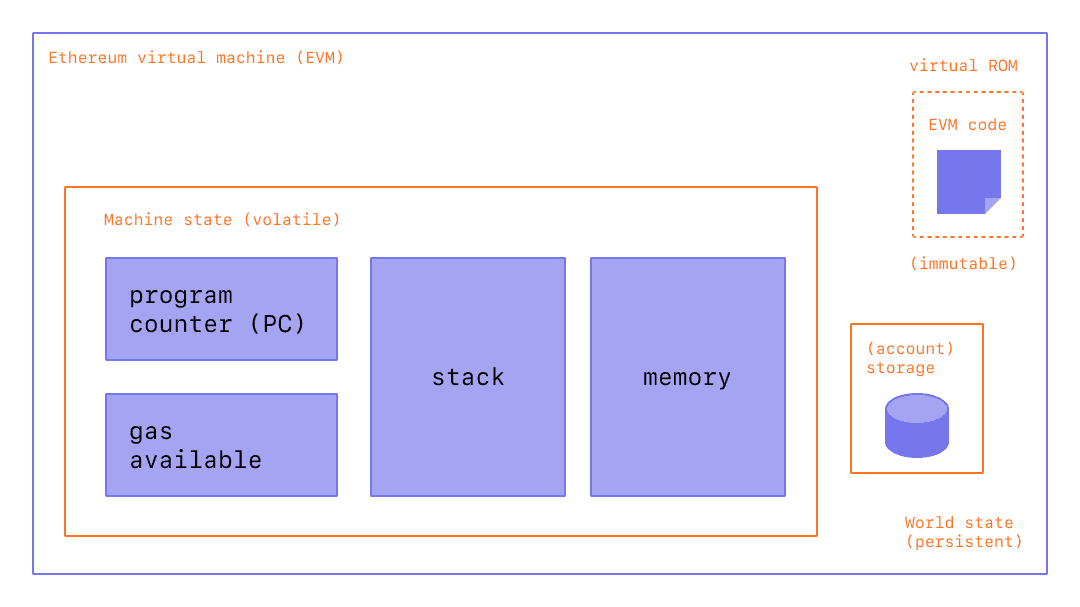
\includegraphics[width=0.8\textwidth]{background/Images/evm.png}
    \caption{EVM components~\cite{noauthor_ethereum_nodate}}
\end{figure}

\subsubsection{Smart Contracts}
Smart contracts are programs that are self-executing contracts between buyers and sellers that deploy on the ethereum network. It allows for the automation of a contract's execution, and can be used to facilitate, verify, and enforce the negotiation or performance of a contract~\cite{noauthor_introduction_nodate, noauthor_smart_nodate}.

\subsection{Decentralised Finance}
One of the main applications of Ethereum and smart contracts are Decentralised Exchanges (DEXes). Before delving into DEXes it is important to understand centralized exchanges.

\subsubsection{Centralized Exchanges}
Centralized exchanges allow agents to discover and trade assets. CEXs ficilitate trading between buyers and sellers by proving an online platform that manages and maintains an order book. An order book aggregates buy and sell orders and executes matching buy and sell orders. The order book and transactions are typically managed on a database as opposed to interacting with the blockchain. When trading, exchanges charge trading fees for the maker and the taker to operate the exchange and do not charge any gas fees as there is no interaction with the blockchain. 

\subsubsection{Decentralized Exchanges}
In contrast, DEXes utilize blockchain technology and smart contracts to execute trades thus providing a high level of determinism. These trades are executed on the blockchain via smart contracts and on-chain transactions. There are two types of DEX, order book DEXes and Automated Market Makers (AMMs). An order book DEX is less common and is similar to CEXs however, the orderbook is stored on the blockchain rather than on a central database. This means each order placed requires the order book to be posted on the block chain at each transaction. Automated Market Makers are more common and provide instant liquidity by using liquidity pools so that users can swap their tokens for a price that is determined by the portions within the liquidity pool~\cite{DEXes}. DEXes have multiple pros including lower transaction fees, privacy, diversity and trustless transactions but they also have their drawbacks such as scalability and poor liquidity are a lot of the DEXes are quite new~\cite{DEXvsCEX}.

\section{Arbitrage}
Arbitrage is the process in which a trader simultaneously buys and sells an asset in order to take advantage of a market inefficiency~\cite{businessinsightsblog_2021}. Arbitrage is also possible in other types of securities by finding price inefficiencies in the prices of options, forward contracts and other exotics.
\\[5mm]
Sources have shown that the word ``\textit{Arbitrage}'' has been used as early as the Renaissance era wehere surviving documents showed a large amount of bills being exchanged~\cite{poitras_2021}. There has also been some evidence to suggest that arbitrage was used as early as the Greek and Roman eras. Objects such as Sumerian cuneiform tablets show trade of ancient bills however we cannot come to strong conclusions of this. Early forms of arbitrage would likely to have been purchasing a commodity then transporting them to a foreign land and selling them at a higher price. This is type of arbitrage is called commodity arbitrage and is still is applicable today. With the example above, transporting the goods takes a significant amount of to the merchant, trader, which could cause variations in the price, however in the modern day this has been reduced and with electronic exchanges this time to buy and sell is very small. This means inefficiencies in the market, where a trader can profit purely by buying and selling, should not exist. This is called the ``Law of One Price''. The ``Law of One Price'' states that every identical commidty or asset should have the same price regardless of exchange or location, given there are no transaction costs, no transportation costs, no legal restrictions, the exchange rates are the same and no market manipulation occurs~\cite{noauthor_law_nodate}. This is because if this were not the case, an arbitrage opportunity would arise and someone would take advantage of the scenario causing the prices on both markets to converge due to the market forces. In the real world arbitrage opportunities are tremendously common, thus allowing a risk-free investment~\cite{10.2307/1828075, RICHARDSON1978341}.
\\[5mm]
There are countless types of arbitrage such as spatial arbitrage, which profits off of different prices on exchanges in different locations, temporal arbitrage, which takes advantage of price differences at different times, risk arbitrage, which proifts from perceived discrepancies in their risk-return profiles and finally market arbitrage which takes advantages of different prices on different exchanges/markets. Statistical methods include pairs trading, which involves buying and selling assets that are believed to be mispriced relative to one another, momentum trading, which identifies if assets have a strong momentum (either up or down) and profiting off of that, and finally algorithmic trading which uses algorithms to analyze data and trades based on statistical analysis. This project shows how these opportunities can be exploited both in a pure manner as well as using statistical methods.

\section{State of Art}
To better understand the project and to be able to research into something new and novel it is important to understand the current state of art, i.e. previous research on the topic. Research into cryptocurrency arbitrage is still in its infancy and previous research has mainly focussed on the economics of cryptocurrencies, i.e. miner/trader behaviour and influence of cryptocurrency trading~\cite{eyal2015miner, avarikioti2020ride, huberman2021monopoly, athey2016bitcoin, easley2019mining, harvey2016cryptofinance, pagnotta2018equilibrium}. Furthermore, there has been very limited research in comparing statistical strategies and pure methods of arbitrage of cryptocurrencies. Despite this, there has been plentiful research on arbitrage as a whole as it is immensly profitable, as a result of this people/institutions tend to keep their newly found research secret. Of the published research, I have looked into the arbitrage techniques that are used. As arbitrage can is highly profitable, it can be found in countless types or assets, such as options, stocks, bonds and many other types of products. Research into all types of products exist going into the theory and practical aspects of each~\cite{mo_theoretical_nodate, 8957853}. The most similar type of asset class to cryptocurrencies is fiat currencies, such as the US Dollar and the Great British Pound Sterling. The research in arbitrage in foreign exchanges show that using a triangular/cyclic arbitrage is highly profitable and effective~\cite{akram2008arbitrage, aiba2002triangular, ito2012free}.

\subsection{Pure Arbitrage Techniques}
As I am using pure arbitrage as a baseline, thus choosing the most optimal stategy is most ideal to better understand the impacts of the optimizations and the statistical stategies themselves. There has been some research on pure arbitrage strategies by finding cyclic opportunities on both centralized and decentralised exchanges, which I go further into in this section.
\\[5mm]
As previously mentioned, research into this topic is still in its infancy thus which means a very thin slice of exploration on the subject matter. Majority of the research has been into the arbitrage on centralized exchanges,~\cite{MakarovIgor2020Taai, crepelliere_arbitrage_2022, PAUNACristian2018ATSf}. These all find massive inefficiencies within these exchanges by finding arbitrage opportunities. One of the more in depth pieces of research, Igor Makarov's and Antoinette Schoar's Trading and arbitrage in cryptocurrency markets~\cite{MakarovIgor2020Taai} finds a large violation in the Law of One Price by finding price discrepencies between the same cryptocurrencies depending on different geolocations. The paper uses 34 exchanges in 19 differing countries, each exchange is grouped accordingly to its location and base currencies, leaving China, Japan, Korea, US, Europe and another group for that uses the Tether, USDT. Within each group the arbitrage index is calculated to compare the maximum difference in prices between exchanges within the same exchange group. This is done by calculating the volume-weighted average price at each exchange, then dividing the maximum price by the minimum price thus if the arbitrage index is 1, then there does not exist an arbitrage opportunity. It is shown that the arbitrage index is over 1 most of the time in all regions thus show a large amount of arbitrage opportunities across different exchanges, with opportunities lasting for as long as several weeks. It is also shown that the arbitrage spreads are consistent and correlated between regions and countries. Although the paper goes into some detail about how one can go about implementing such strategies and it's complications, it didn't implement them thus provides a simply theoretical hypothesis that may or may not work in practice.
\\[5mm]
Cristian Pauna implements an arbitrage strategy in~\cite{PAUNACristian2018ATSf}. The paper details the technical details of arbitrage trading from the data and the system architecture used. Pauna finds complications such as requesting data from multiple exchanges, converting the data such that it is homogeneous and also managing server load. Pauna presents the architecture such that the servers request data from the necessary exchanges, stores them in a relational database which then triggers a server that is used to generate trading signals.

\begin{figure}[!htb]
    \centering
    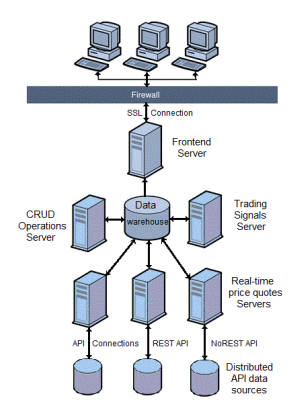
\includegraphics[width=0.28\textwidth]{background/Images/Arbitrage-Architecture.png}
    \caption{Arbitrage system architecture~\cite{PAUNACristian2018ATSf}}
\end{figure}

Now looking at DEXes, research done by Stephen Bryne in his paper,~\cite{byrneexploration} introduces other methods that are commonly used however, not been academically been explored. Methods using properties of ethereum such as using smart contracts for flash loans and buying and selling the same asset in large volumes within the same block in the chain, leading to large profits. The paper details into the technical implementations and issues such as security and reliablity, however it fails to provide analysis and quantitative results on the different methods used to exploit arbitrage opportunities and their differences.
\\[5mm]
As previously mentioned triangular and cyclic arbitrage is one of the most used and purest forms of arbitrage to implement and analyse,~\cite{boonpeam2021arbitrage} explores triangular arbitrage on decentralised exchanges. Algorithm \ref{alg:arb_sys_on_dex} is the algorithm used to find the most profitable arbitrage route on a particular platform, once this is calculated, it is compared with other routes on other platforms. Initially, the system converts the base token into another token and converts it back into the base token, using only one token is used as a middle route, then using the algorithm below, increases the number of middle tokens.

\begin{algorithm}
    \caption{Maximum Profit Route Searching (R)}\label{alg:arb_sys_on_dex}
    \textbf{Input}: $T$ (token list), $P$ (price graph), $n$ (current route)
    \begin{algorithmic}
        \For{$i = 1, ..., T$}
        \State $r = get\_profit(n+i)$
        \For{$j = 1,...,P[i]$}
        \State $p = max(r, R(T, P, n_j))$
        \EndFor
        \EndFor
        \State \textbf{return} $p$
    \end{algorithmic}
\end{algorithm}

\noindent On evaluating the performance of the strategy on differing platforms depended on three main features of each exchange:
\begin{enumerate}
    \item Portion size - Depending on how much the ``trader'' invested revenues differed and infact the larger protion size the revenue decreases as the token pair prices are adjusted based on supply/demand.
    \item Transaction fees - Each exchange has their own transaction fee.
    \item Other considerations such as price slippage - Exchanges have different liquidity levels which depends on the usage and liquidity providers that the exchange employs.
\end{enumerate}

It is found that using this strategy out of the exchanges; Uniswap, 1inch, Kyberswap and Bancor. 1inch was the only exchange that generated a profit whereas the others lose money. The results are shown below on the revenues recieved on each platform experimented on.

\begin{figure}[!htb]
    \centering
    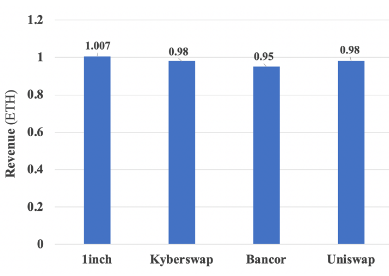
\includegraphics[width=0.5\textwidth]{background/Images/DEXArb_results.png}
    \caption{Trading revenues same token routes within different exchange~\cite{boonpeam2021arbitrage}}
\end{figure}

Another paper that implemented and evaluated a cyclic arbitrage opportunity is~\cite{wang_cyclic_2022}. The research consists of proposing a theoretical arbitrage model and further evaluation on real transactional data. The arbitrage model used is simple to understand, as it searches for a cyclic transaction between $n$ tokens, $A_1, A_2, ..., A_n$ is a sequence of $n$ trades:
\begin{center}
    \begin{minipage}[c]{0.4\linewidth}
        \begin{itemize}
            \item[\textit{Trade 1:}] Exchange $\delta_1$ of $A_1$ to $\delta_2$ of $A_2$
            \item[\textit{Trade 2:}] Exchange $\delta_2$ of $A_2$ to $\delta_3$ of $A_3$
            \item[] $\dotsc$
            \item[\textit{Trade n:}] Exchange $\delta_n$ of $A_n$ to $\delta_1'$ of $A_1$
        \end{itemize}
    \end{minipage}
\end{center}

It is important to note that $\delta_i = \delta_{i+1}$, i.e. the output of a trade is equivelent to the input of the next. The revenues within a cycle are defined as $\delta_{i+1} - \delta_i$, and the overall profit is $\delta_{1}' - \delta_1$. This is not as simple as the revenues obviously depend on how liquid the exchange is, thus the liquidity pools of each possible trading pair is hugely important. Therefore, the paper proposes a theorem, below:

\begin{theorem}
    For a given cycle $A_1 \rightarrow A_2 \rightarrow \cdots \rightarrow A_n \rightarrow A_1$ with $n$ tockens, there exists an arbitrage opportunity for the cyclic transaction if the product of exchange rates $\frac{a_{2,1}a_{3,2}\cdots a_{1,n}}{a_{1,2}a_{2,3}\cdots a_{n, 1}} > \frac{1}{r_1^n r_2^n}$ where $a_{i,j}$ denotes the liquidity of token $A_i$ in the liquidity pool with token $A_j$.~\cite{wang_cyclic_2022}
\end{theorem}

In addition to the theorem, to obtain an optimal strategy we need to compute the optimal trading volume of a cycle, $A_1 \rightarrow A_2 \rightarrow \cdots \rightarrow A_n \rightarrow A_1$. The paper proposes the optimal trading volume to be $\delta^{op}_a = \frac{\sqrt{r_1 r_2 a' a} - a}{r_1}$ where $a = \frac{a_{1,n}'a_{n,1}}{a_{n,1}+r_1 r_2 a_{n,1}'}$ and $a' = \frac{r_1 r_2 a_{1,n}'a_{n,1}}{a_{n,1}+r_1 r_2 a_{n,1}'}$. Thus in order to calculate such arbitrage opportunities knowing the liquidity of tokens in other tokens' liquidity pools, algorithm \ref{alg:liquidity_alg} infers the direction and volumes to trade to get the optimal revenue.

\begin{algorithm}
    \caption{Computing the equivelent liquidity of the cycle}\label{alg:liquidity_alg}
    \begin{algorithmic}
        \State $a_{1, n}' \leftarrow a_{1,2}$
        \State $a_{n, 1}' \leftarrow a_{2,1}$
        \For{$i$ from $2$ to $n-1$}
        \State $a_{1, n}' \leftarrow \frac{a_{1,n}'a_{i,i+1}}{a_{i,i+1}+r_1 r_2 a_{n,1}'}$
        \State $a_{n, 1}' \leftarrow \frac{r_1 r_2 a_{1,n}'a_{i+1, i}}{a_{i,i+1}+r_1 r_2 a_{n,1}'}$
        \EndFor
    \end{algorithmic}
\end{algorithm}

After analysis, it is found that between 4th May 2020 to 15th April 2021, there were countless exploitable arbitrage opportunities and in fact grew to 1,750 in the 11 months that it was tested on. Only cycles with length 3 were experimented with and only cycles including ETH as 80\% of the liquidity pools on Uniswap include ETH and another cryptocurrency~\cite{heimbach2021behavior}. Furthermore, it is found that 287,241 of the 292,606 arbitrages executed started with ETH, 85\% of the arbitrages used a cycle of length 3. The total revenue of the cyclic arbitrage was 34,429 ETH. However, gas fees accounts for 24.6\% of the total revenue leaving an approximate 25,971 ETH profit.
\\[5mm]
% \vspace{5mm}
The paper then delves into the implementation of the smart contract, the paper explored how both \textit{sequential} and \textit{atomic} implementations would affect the revenue and execution of the contracts. It was found that 52.3\% of the arbitrages that were executed sequentially generated a loss, likely due to the fact when one submits $n$ orders, the $n$ blockchain transactions are executed sequentially, meaning some external transactions can be inserted between these transactions. Thus using atomic transactions avoids this issue of external transactions do not effect the market price that may effect the outcome of the arbitrage.
\\[5mm]
Furthermore, the authors of the paper also investigated the performance differences of using private smart contracts and public contracts. Deploying a smart contract that calls Uniswap functions, i.e. a private smart contract, is intuitively better and achieves a higher success rate of a lower bound of 52\% and a higher bound of 90\% in comparison to calling a public Uniswap smart contract which has success rate of 27.3\%. Overall the paper provides an insightful look into cyclic arbitrage in DEXes and highlights important decisions made such as liquidity calculations and smart contracts, while comparing the performance of differing options available.

\subsection{Statistical Arbitrage Techniques}

As mentioned previously mentioned and the subject of the project is to optimize statistical arbitrage methods to be able to compete with a more purer form of arbitrage, i.e. cyclic arbitrage. As previously mentioned there are many methods of stat arb, pairs trading, momentum trading and algorithmic trading. Within these methods there are countless strategies to adopt and profit off of, thus to limit the scope, this project I will be investigating strategies within pair trading. Research within Pair trading has been vast with many streams of approaches emerging; distance approach, cointegration approach, time-series approach, stochastic approach and some others, including using machine learning~\cite{https://doi.org/10.1111/joes.12153}.
\\[5mm]
The distance approach is easy to understand; using the euclidian squared difference of combinations historical normalized prices of assets from a selected time period and selecting the top 20 pairs of assets with the least historical distance. Once pairs are selected, monitor the prices and if the prices diverge by over 2 standard deviations, buy the undervalued asset and sell the overvalues asset and when the prices converge, close the position~\cite{RadLowFaff}. This is called Mean reversion and is fundemental technique used in pairs trading.
\\[5mm]
The cointegration approach follows three key steps. The first being selection of pairs based on similarity measures, the next being assessing the tradability and finally thresholds are set for trading. The spread is defined as $$\varepsilon_{i j,t} = P_{i,t} + \gamma P_{j,t}$$ where $P_{i,t}$ and $P_{j,t}$ denote the $I(1)$ non-stationary price processes of the assets $i$ and $j$, $\gamma$ is the cointegration coefficient, also refered to in literature as the hedge ratio. $\varepsilon_{i j,t}$ is the linear combination of the non-stationary prices and is $I(0)$ stationary and hence mean-reverting, note that stationary processes are those of which have a constant mean. Rad's implementation of this approach on stocks result in a 0.83\% return before considering transaction costs~\cite{RadLowFaff}. Another paper,~\cite{lossProtection}, looked into setting the thresholds and setting a minimum profit, $MP_{ij,t_c}$: $$MP_{ij,t_c} = \frac{n(\varepsilon_{i j,t_0} - \varepsilon_{i j,t_c})}{ \mid \gamma \mid}$$ Where $t_0$ and $t_c$ are the opening and closing times, $n$ is the volume longed of asset $j$.
\\[5mm]
There has been further research into optimizing mean reversion, one of which was to use the successive convex approximation method on the mean reverting portfolio design ~\cite{ZipingZhao2019OMPW}. The paper initially proposes the mean reversion portfolio:
\begin{itemize}
    \itemsep0em
    \item For each asset, the price at time $t$ is denoted as $p_t$ and its correspondeing log-price $y_t \triangleq log(p_t)$, its vector form of $M$ assets $\mathbf{y}_t \triangleq \big[ y_{1,t}, \dots ,y_{M,t} \big]^T$.
    \item The log-price spread is given by $y_t \triangleq \mathbf{\beta}^T\mathbf{y}_t$, where $\mathbf{\beta} \triangleq \big[ \beta_1, \dots ,\beta_M \big]^T$ denotes the hedge ratios.
    \item The cointegration space with $N$ relations is defined by $\mathbf{B} \triangleq \big[ \beta_1, \dots ,\beta_N \big]$, thus the $N$ spreads are $s_t \triangleq \mathbf{B}^T\mathbf{y}_t$.
    \item For these $N$ spreads, the portfolio weight matrix is denoted as $\mathbf{w} \triangleq \big[ w_1, \dots ,w_N \big]^T$.
    \item The auto-covariance matrix for the spreads $s_t$ is defined as \\ ${M_i \triangleq Cov(s_t, s_{t+i}) = \mathop{\mathbb{E}} \big[ \big( s_t - \mathop{\mathbb{E}} \big[ s_t \big]\big) \big( s_{t+i} - \mathop{\mathbb{E}} \big[ s_{t+i} \big]\big)^T \big]}$
\end{itemize}

\noindent Now that we have defined everything required, we can now formulize the problem. The general problem of mean reversion portfolio design problem is formalized by:
\begin{equation*}
    \begin{aligned}
         & \underset{\mathbf{w}}{\text{minimize}}
         &                                        & F(\mathbf{w}) \triangleq U(\mathbf{w}) + \mu V(\mathbf{w}) + \gamma S(\mathbf{w})                                                                       \\
         & \text{subject to}
         &                                        & \mathbf{w} \in \biggl\{ \mathbf{w} \mid \big\| \mathbf{B} \mathbf{w}\big\|_0 \leq L \biggr\}, \qquad \text{where $L$ is the total leveraged investment}
    \end{aligned}
\end{equation*}

\begin{itemize}
    \item $\mu$ defines the trade-off between the mean reversion measure and the variance preference.
    \item $\gamma$ defines the regularization parameter of how sparse we would like the cointegration space to be.
\end{itemize}

\noindent Where the Mean Reversion term: $$U(\mathbf{w}) \triangleq \xi \frac{\mathbf{w}^T \mathbf{H}\mathbf{w}}{\mathbf{w}^T \mathbf{M}_0\mathbf{w}} + \zeta \biggl( \frac{\mathbf{w}^T \mathbf{M}_1\mathbf{w}}{\mathbf{w}^T \mathbf{M}_0\mathbf{w}} \biggr) ^2 + \eta \sum_{i=2}^{p} \biggl( \frac{\mathbf{w}^T \mathbf{M}_i\mathbf{w}}{\mathbf{w}^T \mathbf{M}_0\mathbf{w}}\biggr)^2$$ And the variance term: $$V(\mathbf{w}) \triangleq \begin{cases}
        1/\mathbf{w}^T \mathbf{M}_0\mathbf{w}        & \text{VarInv(\textbf{w})} \\
        1/\sqrt{\mathbf{w}^T \mathbf{M}_0\mathbf{w}} & \text{StdInv(\textbf{w})} \\
        -\mathbf{w}^T \mathbf{M}_0\mathbf{w}         & \text{VarNeg(\textbf{w})} \\
        -\sqrt{\mathbf{w}^T \mathbf{M}_0\mathbf{w}}  & \text{StdNeg(\textbf{w})}
    \end{cases}$$
The variance term can be represented in any of the four forms.
\\[5mm]
And the asset selection term: $$S(\mathbf{w}) \triangleq \big\| \mathbf{B} \mathbf{w}\big\|_0 = \sum_{m=1}^{M} sgn(\mid \bigl[ \mathbf{B} \mathbf{w} \bigr]_m \mid)$$ This asset selection critorian is not necessary however as trading incur a cost, selecting all of the asset is costly, thus selecting a subset of assets to trade is more profitable. To formulize this goal, we would like to minimize the cointegration space thus we use the $\ell_0$ norm.
\\[5mm]
The paper then goes on to solve the optimization problem using the successive convex approximation (SCA) method~\cite{scaOptimization}. The SCA method takes an optimization problem in the form of:
\begin{equation*}
    \begin{aligned}
         & \underset{\mathbf{x}}{\text{minimize}}
         &                                        & f(\mathbf{x})              \\
         & \text{subject to}
         &                                        & \mathbf{x} \in \mathcal{X}
    \end{aligned}
\end{equation*}
\noindent Where $\mathcal{X} \subseteq \mathbb{R}^N$ is convex and $f(\mathbf{x})$ is non-convex. The SCA method involves starting at an initial point $\mathbf{x}^{(0)}$ and solving a series of subproblems of surrogate funtions $\tilde{f}(\mathbf{x}; \mathbf{x}^{(k)})$ over the set $\mathcal{X}$. The sequence $\bigl\{ \mathbf{x}^{(k)} \bigr\}$ is generated by: $$\begin{cases}
        \hat{\mathbf{x}}^{(k+1)} = arg \underset{\mathbf{x} \in \mathcal{X}}{min} \tilde{f}(\mathbf{x}; \mathbf{x}^{(k)}) \\
        \mathbf{x}^{(k+1)} = \mathbf{x}^{(k)} + \gamma^{(k)}(\hat{\mathbf{x}}^{(k+1)} - \mathbf{x}^{(k)})
    \end{cases}$$
The first step is to generate a descent direction and then update the variable with a step size of $\gamma^{(k)}$. After applying this method to the MRP problem and further analysis the paper, the following algorithm is proposed and used to solve the MRP design problem:
\begin{algorithm}
    \caption{SCA-Based Algorithm for The Optimal MRP Design Problem}\label{alg:sca_alg}
    \textbf{Require}: $\mathbf{H}, \mathbf{M}_i, \mu, \gamma, \mathbf{B}, L \text{ and } \tau$
    \begin{algorithmic}[1]
        \State Set $k=0, \gamma^{(0)}$ and $\mathbf{w}^{(0)}$
        \Repeat
        \State Compute $\mathbf{A}^{(k)}$ and $\mathbf{b}^{(k)}$
        \State $\hat{\mathbf{w}}^{(k+1)} = arg \underset{\mathbf{w} \in \mathcal{W}}{min} \mathbf{w}^{T}\mathbf{A}^{(k)}\mathbf{w} + \mathbf{b}^{(k)T}\mathbf{w}$
        \State $\mathbf{w}^{(k+1)} = \mathbf{w}^{(k)} + \gamma^{(k)}(\hat{\mathbf{w}}^{(k+1)} - \mathbf{w}^{(k)})$
        \State $k \leftarrow k+1$
        \Until convergence
    \end{algorithmic}
\end{algorithm}

\noindent However, 4 line is a convex problem and has no closed form solution thus to solve this subproblem using the ADMM method, this is done by introducing an auxilary variable $\mathbf{z = Bw}$.
\begin{equation*}
    \begin{aligned}
         & \underset{\mathbf{x, z}}{\text{minimize}}
         &                                           & \mathbf{w}^{T}\mathbf{A}\mathbf{w} + \mathbf{b}^{T}\mathbf{w} \\
         & \text{subject to}
         &                                           & \big\| \mathbf{z} \big\|_1 \leq B, \mathbf{Bw - z=0}
    \end{aligned}
\end{equation*}
\noindent This is then summerized into Algorithm \ref{alg:admm_alg}:
\begin{algorithm}
    \caption{An ADMM-Based Algorithm for Problem on line 4 in Algorithm \ref{alg:sca_alg}}\label{alg:admm_alg}
    \textbf{Require}: $\mathbf{A}, \mathbf{b}, \mathbf{B}, B, \rho$
    \begin{algorithmic}[1]
        \State Set $\mathbf{w}^{(0)}, \mathbf{z}^{(0)}, \mathbf{u}^{(0)}$ and $k=0$
        \Repeat
        \State $\mathbf{w}^{(k+1)} = -(2\mathbf{A} + \rho \mathbf{B}^T\mathbf{B})^{-1}(\mathbf{b} + \rho \mathbf{B}^T(\mathbf{u}^{(k)} - \mathbf{z}^{(k)}))$
        \State $\mathbf{h}^{(k)} = \mathbf{Bw}^{(k+1)} + \mathbf{u}^{(k)}$
        \State $\mathbf{z}^{(k+1)} = \Pi_{\mathcal{C}}(\mathbf{h}^{(k)})$
        \State $\mathbf{u}^{(k+1)} = \mathbf{u}^{(k)} + \mathbf{Bw}^{(k+1)} - \mathbf{z}^{(k+1)}$
        \State $k \leftarrow k+1$
        \Until convergence
    \end{algorithmic}
\end{algorithm}

\noindent After all of this analysis, the authors of the paper, \cite{8450775, ZipingZhao2019OMPW}, ran simulations on real data comparing underlying spread. It found that it resulted in consistent profits as shown in figure \ref{fig:ROIsMRP}:

\begin{figure}[htb!]
    \centering
    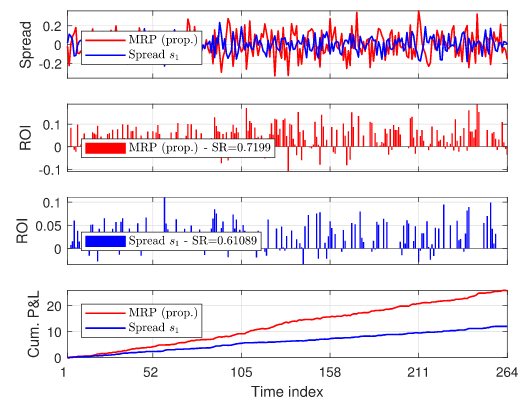
\includegraphics[width=0.4\textwidth]{background/Images/rois1.png}
    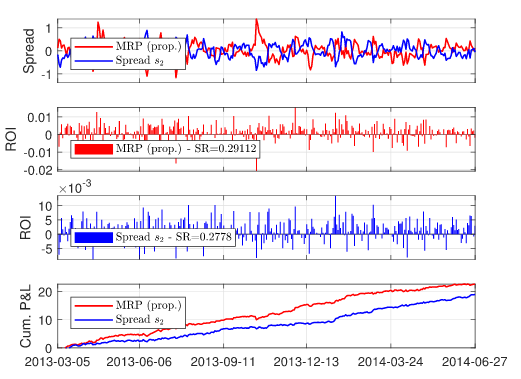
\includegraphics[width=0.43\textwidth]{background/Images/rois2.png}
    \caption{A mean-reversion trading based on real data~\cite{ZipingZhao2019OMPW}}
    \label{fig:ROIsMRP}
\end{figure}

\noindent Overall, this research succesfully formulizes, solves the optimization problem mathematically, and goes further to implement the algorithms to solve the problem programmatically. In addtion, the author compares the implementation with other benchmark algorithms, showing that it results in a greater P\&L and sharpe ratio.
\\[5mm]
Although, the research in the papers previously mentioned do not investigate the cointegration approach on cryptocurrencies, the takeaways are the mathematical fundementals that are used in statistical arbitrage. Kristoufek and Bouri researched into the sources of stat. arb. of bitcoin in multiple centralized exchanges. The Grey correlation is built on top of the Grey system theory~\cite{JULONG1982288}, and is able to capture non-linear correlations without assuming a Gaussian distribution, thus using Grey correlation provides a more robust metric to understand correlations between series'. The Grey correlation $\gamma(X_0, X_i)$ is defined with two steps:
\begin{enumerate}
    \item $\gamma(x_0(k), x_i(k)) = \frac{min_i min_k \mid x_0(k) - x_i(k) \mid + \varepsilon max_i max_k \mid x_0(k) - x_i(k) \mid}{\mid x_0(k) - x_i(k) \mid + \varepsilon max_i max_k \mid x_0(k) - x_i(k) \mid}$
    \item $\gamma(X_0, X_i) = \frac{1}{n} \sum_{i=1}^{n} \gamma(x_0(k), x_i(k))$
\end{enumerate}
\noindent With $\varepsilon \in [0,1]$, the standard is set to $\varepsilon = 0.5$.
\\[5mm]
The DCC-GARCH(1,1), \cite{engle2002dynamic}, model also used to obtain conditional correlations for Bitcoin exchanges. The model was designed to used a combination of parameters such as the standard deviation of Bitcoin returns, traded volume, volume of on-chain transactions, fees paid to miners, ratio of current price and recent price history and internet hype/trends.
\\[5mm]
Upon analysis of Grey and DCC-GARCH(1,1) correlations, it is found that the DCC correlations show a little variability whereas the Grey correlations being a lot more variable ranging from 0.29 to 1. In addition, the paper then further investigates these sources and finds that these opportunities are introduced when there is a large number of inter-exchange tranfer requests, i.e. the network is congester, and high price volitility. In contrast, high volume of exchanges and on-chain activity cause the arbitrage opportunities to decrease. This paper finds and explains these sources of statistical arbitrage however does not implement or devise an algorithm that uses statistical arbitrage to generate a profit from price discrepancies of Bitcoin on different exchanges.
\\[5mm]
A paper that investigates statistical arbitrage on multiple cryptocurrencies is \cite{Figa-TalamancaGianna2021Cdff}. The authors of this paper analysed co-movements and cointegration of different cryptocurrencies on a centralized exchange using Augmented Dickey Fuller (ADF) and  Kwiatkowsky-Phillips-Schmidt-Shin (KPSS), Ljung-Box autocorrelation tests on both stationary form ($I(0)$) and the original form ($I(1)$). The paper then develops a dynamic factor model based on the assumption that the price dynamics of cryptocurrencies is driven by Bitcoin~\cite{blau2020comovement}, this is then evidenced by similar paths found in cryptocurrencies shown in Figure \ref{fig:pricebehaviour}.
\begin{figure}[h!]
    \centering
    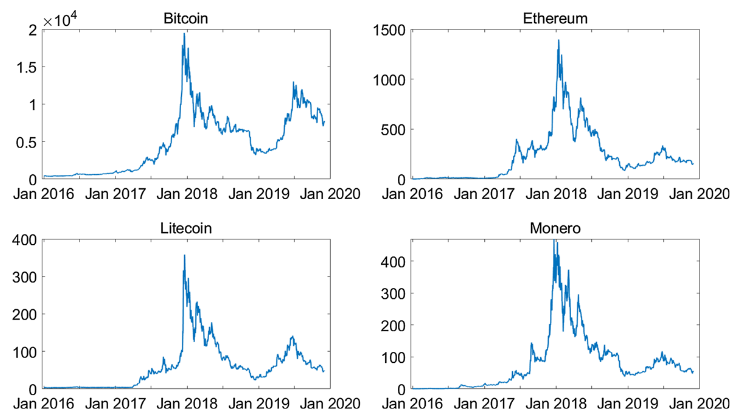
\includegraphics[width=0.8\textwidth]{background/Images/price_behaviour.png}
    \caption{Price behaviour of Bitcoin, Ethereum, Litecoin, Monero~\cite{Figa-TalamancaGianna2021Cdff}}
    \label{fig:pricebehaviour}
\end{figure}

\noindent For simplicity the authors set the number of hidden factors to 2 and upon analysis $f_1$ is a $I(1)$ process and the second factor $f_2$ is a stationary process that is independent from $f_1$. It is also found after overlaying $f_1$ with the price of Bitcoin, that the first factor strongly correlates with the price of Bitcoin.

\begin{figure}[h!]
    \centering
    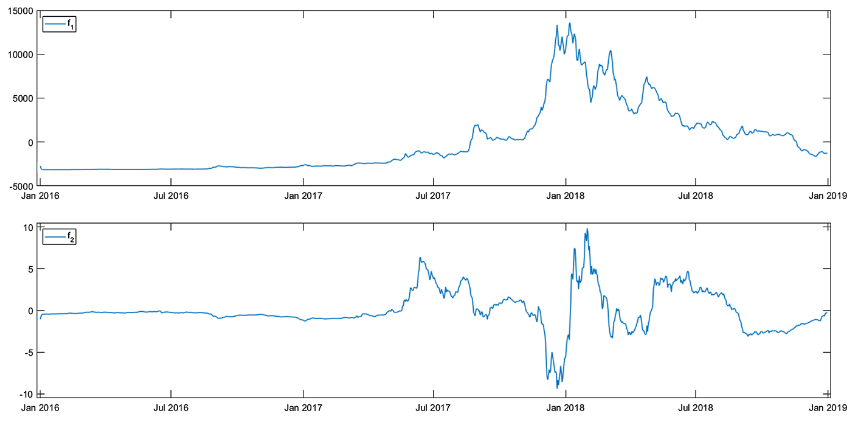
\includegraphics[width=0.8\textwidth]{background/Images/hidden_factors.png}
    \caption{Hidden factors $f_1$ and $f_2$ from Jan 2016 to Dec 2018~\cite{Figa-TalamancaGianna2021Cdff}}
    \label{fig:hiddenfactors}
\end{figure}

\noindent The paper then uses this model to build an investment strategy, using forecasting using the estimated parameters:
$$\hat{p}_{i, \tau + 1} = \mathbb{E}_{\tau}(p_{i, \tau + 1}) = \hat{\alpha_i} + \hat{\beta}_{i 1} \mathbb{E}_{\tau}(f_{1, \tau + 1}) + \hat{\beta}_{i 2} \mathbb{E}_{\tau}(f_{2, \tau + 1}) $$
Where
$$f_{1, t} = \lambda_1 f_{1, t-1} + \eta_{1,t}$$
$$f_{2, t} = \lambda_2 f_{2, t-1} + \eta_{2,t}$$
The expected gains one day ahead is given by:
$$g_{\tau + 1} =  \mathbb{E}_{\tau}[v_{\tau + 1}] = \sum_{i=1}^{\lfloor I / 2 \rfloor} \hat{p}_{\tau + 1}^{(i)} - \sum_{i=\lceil I / 2 \rceil + 1}^{I} \hat{p}_{\tau + 1}^{(i)} $$

\noindent Using this and a thresholds which are calculated by the combination of the current price and standard deviation of the trading position value:
\begin{itemize}
    \itemsep0em
    \item if $g_{\tau + 1} > v_{\tau} + c \sigma_{\tau}^v$, go long
    \item if $g_{\tau + 1} < v_{\tau} - c \sigma_{\tau}^v$, go short
    \item if $v_{\tau} - c \sigma_{\tau}^v \leq g_{\tau + 1} \geq v_{\tau} + c \sigma_{\tau}^v$, no trade
\end{itemize}

\noindent The researchers of the paper evaluated their trading strategy for 334 days and a moving window of 3 years, 1096 observations, every day to estimate the parameters for the dynamic factor model. We can see in Figure \ref{fig:gains} that the strategy was able to consistently generate a profit even when considering transaction costs.

\begin{figure}[htb!]
    \centering
    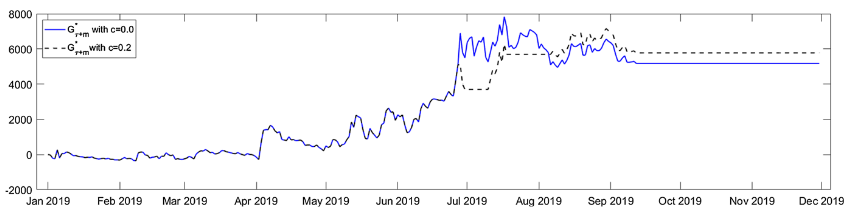
\includegraphics[width=0.8\textwidth]{background/Images/gains.png}
    \caption{Net gains taking transaction fees into account~\cite{Figa-TalamancaGianna2021Cdff}}
    \label{fig:gains}
\end{figure}

\noindent Another method that is used in statistical arbitrage is using the Kalman Filter. Recall the equation for spread:
$$\varepsilon_{i j,t} = P_{i,t} + \gamma P_{j,t}$$
\noindent The Kalman filter is a recursive algorithm for estimating the sate of data that is usually very noisy and thus needs to be filtered~\cite{ALSADIK2019299}. This makes it very useful to estimate the hedge ratio $\gamma$. Initially, a book by Vidyamurthy discusses best practices for choosing cointegrated equities and found that the kalman filter was found optimal when the state-space and observation equations are linear and the noise is Gaussian~\cite{vidyamurthy2004pairs}. Since then there has been many extensions of the filter such as the Extended Kalman Filter (EKF) and Unscented KF aimed to handle when the state-space and observation equations are non-linear and the noise is not Gaussian.
\\[5mm]
The Kalman Filter works in 2 phases, prediction and update. The prediction phase is as follows $$\hat{\mathbf{x}}_k = \mathbf{F}_k \hat{\mathbf{x}}_{k-1} + \mathbf{B}_k \overset{\rightarrow}{\mathbf{u}}_k + \mathbf{w}_k$$ $$\mathbf{P}_k = \mathbf{F}_k \mathbf{P}_{k-1} \mathbf{F}_k^T + \mathbf{Q}_k $$ Where $\hat{\mathbf{x}}_k$ is the new best estimate (prediction) that is derived from $\hat{\mathbf{x}}_{k-1}$, the previous estimate and the prediction function $\mathbf{F}_k$. $\overset{\rightarrow}{\mathbf{u}}_k$ is the correction term, called the control vector, that is used when it is known that there are external influences in combination with $\mathbf{B}_k$ which is called the control matrix. In addition to this, the new uncertainty (covariance matrix), $\mathbf{P}_k$, is calculated using the previous uncertainty and additional uncertainty from the environment, $\mathbf{Q}_k $, $\mathbf{w}_k$ is called the state noise. The update is as follows $$\hat{\mathbf{x}}_k' = \hat{\mathbf{x}}_k + \mathbf{K}'(\overset{\rightarrow}{\mathbf{z}}_k - \mathbf{H}_k \hat{\mathbf{x}}_k)$$ $$\mathbf{P}_k' = \mathbf{P}_k - \mathbf{K}'\mathbf{H}_k \mathbf{P}_k$$ $$\mathbf{K}' = \mathbf{P}_k \mathbf{H}_k^T (\mathbf{H}_k \mathbf{P}_k \mathbf{H}_k^T + \mathbf{R}_k)^{-1}$$ Where $\mathbf{K}'$ is defined as the Kalman gain, $\mathbf{H}_k$ is the measurement matrix, $\overset{\rightarrow}{\mathbf{z}}_k$ is mean of the observed values, which is also calculated by $\overset{\rightarrow}{\mathbf{z}}_k = \mathbf{H}_k \hat{\mathbf{x}}_k + \mathbf{v}_k$ where $\mathbf{v}_k$ is the measurement noise, and $\mathbf{R}_k$ is the covariance of the uncertainty of the observed values~\cite{kalman_filter_bzarg}.
\\[5mm]
A paper that investigated the use of the Kalman Filter on ETFs found that the strategy it employed worked well for in-sample data points and worse, but still profitable, results of out-of-sample data. The paper adapted the Kalman Filter to be able to use it for pairs trading to the following: $$\mathbf{y}_t = \mathbf{x}_t \mathbf{\beta}_t + \mathbf{\epsilon}_t$$ $$\mathbf{\beta}_t = \mathbf{I} \mathbf{\beta}_{t-1} + \mathbf{\omega}_t$$ Then calculating the Kalman Gain: $$\text{Kalman Gain} = \frac{\text{Error in the estimate}}{\text{Error in the estimate + Error in the measurement}}$$ Then to calculate the estimate: $$\text{Estimate}_t = \text{Estimate}_{t-1} + \text{Kalman Gain} \times (\text{Measurement - }\text{Estimate}_{t-1})$$ And finally, calculating the new error: $$E_{\text{estimate}_t} = \frac{E_{\text{measurement}} \times E_{\text{estimate}_{t-1}}}{E_{\text{measurement}} + E_{\text{estimate}_{t-1}}}$$ $$E_{\text{estimate}_t} = E_{\text{estimate}_{t-1}} \times (1 - \text{Kalman Gain})$$

\noindent The paper later hypothesises the causes for the disappointing results to the ``pairs trading strategies have gained widespread acceptance thus making profitability much more elusive'', however the author fails to find evidence or provide sufficient evidence to justify the claim~\cite{dempsey_market_2017}.
\begin{figure}[htb!]
    \centering
    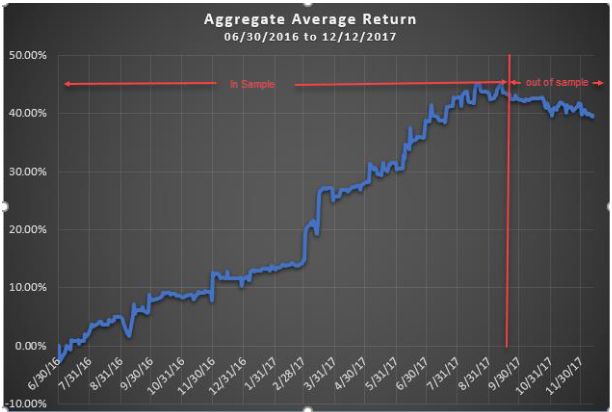
\includegraphics[width=0.8\textwidth]{background/Images/insamplevsoutsampleresults.png}
    \caption{Aggregate average return of using the kalman filter for pairs trading on ETFs~\cite{dempsey_market_2017}}
    \label{fig:kalman_results}
\end{figure}
\\[5mm]
Another paper used the combination of the Kalman Filter and Machine Learning, more specifically Extreme Learning Machine and Support Vector Regression (SVR) to build a statistical arbitrage strategy on the Brazilian Stock Exchange. The strategies can simply be explained as using SVR and ELM to forcast returns and using the Kalman Filter to improve the forcast.
\begin{figure}[htb!]
    \centering
    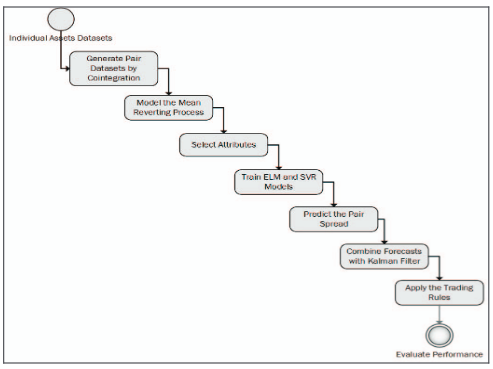
\includegraphics[width=0.8\textwidth]{background/Images/KalmanMLFlowChart.png}
    \caption{Visualisation of the trading strategy used in \cite{6974093}}
    \label{fig:kalman_ml_flowchart}
\end{figure}
\\[5mm]
The paper also compares methods, such as LASSO, BMA, GRR, to benchmark the performance of the Kalman Filter. The research found that using simply ELM and SVR forcasts result in a return of 20.19\% and 21.32\% respectively for out-of-sample data points and by using a combination with the Kalman Filter give a return of 26.13\% for out-of-sample data points. The full results can be seen below in Figure \ref{fig:kalman_ml_results}. In addition to this it can be seen that the volitility of the return also decreases which is ideal for investment managers.
\begin{figure}[htb!]
    \centering
    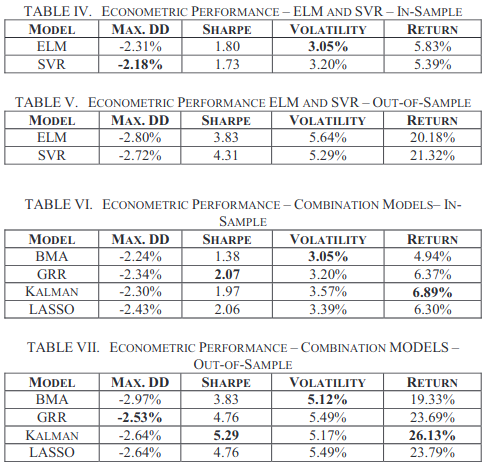
\includegraphics[width=0.6\textwidth]{background/Images/kalman_ml_results.png}
    \caption{Econometric results~\cite{6974093}}
    \label{fig:kalman_ml_results}
\end{figure}
\\[5mm]
Other papers/articles such as \cite{KRAUSS2017689, alma991000475380901591, jrfm12010031} have designed, compared and analysed other statistical arbitrage techniques using Machine Learning algorithms and revealed that some algorithms are profitable. The majority of research on machine learning trading strategies has been on assets such as stocks on centralized exchanges. The little research that has been done on statistical arbitrage on cryptocurrencies has all been on analysing arbitrage on centralized exchanges and not decentralised exchanges. One of the research projects that analysed machine learning methods of statistical arbitrage on cryptocurrencies on a centralized exchange, compared a logistic regression approach with a random forest approach~\cite{jrfm12010031}. 

%%%%%%%%%%%%%%%%%%%%%%%%%%%%%%%%%%%%%%%%%%%%%%%%%%%%%%%%%%%%%%%%%%%%%%%%%%%%%%%%%%%%%%%%%%%%%%%%%%%%%%%%%%%%%%%%%%%%%%%%%%%%%%%%%%%%%%%%%%%%%%%%%%%%%%%%%%%%%%%%%%%%%%%%%%%%%%%%%%%%%%%%%%%%%%%%%%%%%%%%%%%%%%%%%%%%%%%%%%%%%%%%%%%%%%%%%%%%%%%%%%%%%%%%%%%

% \textbf{Ones that use ML:}
% \begin{itemize}
%     \item Statistical Arbitrage in Cryptocurrency Markets \cite{jrfm12010031} %file:///home/devam/Documents/Imperial/Year_4/Individual%20Project/Interim%20Report/background/Articles/Statistical%20Arbitrage%20in%20Cryptocurrency%20Markets%20.pdf
%     \item Deep neural networks, gradient-boosted trees, random forests: Statistical arbitrage on the S\&P 500 \cite{KRAUSS2017689} %file:///home/devam/Documents/Imperial/Year_4/Individual%20Project/Interim%20Report/background/Articles/Deep_neural_networks,gradient-boosted_trees,random_forests:_Statistical_arbitrage_on_the_S&P_500.pdf
%     \item A Machine Learning based Pairs Trading Investment Strategy \cite{alma991000475380901591} %file:///home/devam/Documents/Imperial/Year_4/Individual%20Project/Interim%20Report/background/Articles/A%20Machine%20Learning%20based%20Pairs%20Trading%20Investment%20Strategy%20.pdf
% \end{itemize}

% \textbf{Broader Picture}
% \begin{itemize}
%     \item STATISTICAL ARBITRAGE PAIRS TRADING STRATEGIES: REVIEW AND OUTLOOK \cite{https://doi.org/10.1111/joes.12153} %file:///home/devam/Documents/Imperial/Year_4/Individual%20Project/Interim%20Report/background/Articles/Journal%20of%20Economic%20Surveys%20-%202016%20-%20Krauss%20-%20STATISTICAL%20ARBITRAGE%20PAIRS%20TRADING%20STRATEGIES%20REVIEW%20AND%20OUTLOOK.pdf
%     \item Statistical Arbitrage: Algorithmic Trading Insights and Techniques \cite{alma991000607977501591} %file:///home/devam/Documents/Imperial/Year_4/Individual%20Project/Interim%20Report/background/Articles/Statistical%20arbitrage%20:%20algorithmic%20trading%20insights%20and%20techniques.pdf
% \end{itemize}



% WowSwap, dydx, gmx, ... https://defiprime.com/margin-trading
% https://corporatefinanceinstitute.com/resources/cryptocurrency/cryptocurrency-exchanges/
% https://wowswap-io.medium.com/the-big-short-introducing-decentralized-leveraged-short-swaps-a81eb9d1c36f 
% https://defiprime.com/margin-trading
% https://github.com/evbots/dex-protocols
% 
% https://medium.com/defi-saver/how-to-long-or-short-any-asset-using-defi-lending-protocols-812300c9a640
% https://defiprime.com/exchanges

% https://www.youtube.com/watch?v=zABaCh3yAho - video on markovian auto regressive methods
% https://medium.com/@rachita.pateria/an-introduction-to-markov-switching-model-for-time-series-b279e9e26125

% \begin{enumerate}
%     \item \cite{HuangJianfeng2022Taaf} - %https://library-search.imperial.ac.uk/permalink/44IMP_INST/fv0fdm/cdi_informaworld_taylorfrancis_310_1080_13504851_2021_1930998
%     \item \cite{alma991000411969901591} - %https://library-search.imperial.ac.uk/permalink/44IMP_INST/mek6kh/alma991000411969901591
%     \item \cite{} - %https://library-search.imperial.ac.uk/permalink/44IMP_INST/mek6kh/alma991000343762601591
%     \item \cite{} - %https://library-search.imperial.ac.uk/permalink/44IMP_INST/mek6kh/alma996037714401591
%     \item \cite{} - %https://library-search.imperial.ac.uk/permalink/44IMP_INST/mek6kh/alma991000617323401591
% \end{enumerate}


\chapter{Design Decisions}

\section{Mean Reversion Strategies}
Considering the current state of the art and the limited exploration of statistical arbitrage in decentralized exchanges, the objective of this project is to examine the profitability of mean reversion techniques in pairs trading and determine if they offer a viable investment opportunity. Additionally, by employing various methods to estimate the hedge ratio and effectively manage risk, we can further analyze the overall performance and appeal of the trading strategy to potential traders.
\\[5mm]
In the mean reversion strategies, the hedge ratio refers to the ratio or proportion between the positions of two assets involved in a pairs trading strategy. It determines the optimal allocation of capital between the assets to minimize risk and create a market-neutral position. The hedge ratio represents the number of units or shares of one asset that should be held for each unit or share of the other asset in order to create a balanced or hedged position. It is derived through statistical techniques such as regression analysis. The methods that are explored in this paper are the use of a Constant Hedge Ratio, Sliding Window Ordinary Least Squares, Lagged Ordinary Least Squares, the unrestricted OLS model returned by the Granger Causality Test and also the Kalman Filter. These methods are selected due to their ability to test whether underlying dynamics effect the relationships between liquidity pools, hence effecting the hedge ratio. To further see the details and implementation of each strategy, refer to Section \ref{sec:strats}.

\section{Buying and Selling}
\label{sec:buying-selling}
The process of buying and selling in traditional markets is relatively straightforward as brokers and exchanges play a crucial role in executing orders on behalf of individuals. However, when it comes to trading cryptocurrencies, the responsibility falls directly on the trader, such as myself. Therefore, it becomes essential to clearly define what buying and selling entail in the context of cryptocurrency trading.

\subsection{Buying}
Prices on Uniswap are represented as ratios for example 1 USDC = $P$ WETH. With this understanding, let's delve into the process of buying one unit of USDC/WETH on Uniswap:
\begin{itemize}
    \item Opening a Buy position:\begin{itemize}
        \item Starts with $P_{0}$ WETH
        \item Swaps the WETH for USDC, hence ends with 1 USDC
    \end{itemize}
    \item Closing a Buy position:\begin{itemize}
        \item Starts with 1 USDC
        \item Swaps the USDC for WETH, hence ends with $P_1$ WETH
    \end{itemize}
\end{itemize}
\noindent Consequently, if the price of USDC/WETH increases from the moment the buy position is opened to the time it is closed, the trader realizes a profit. On the other hand, if the price declines during this period, the trader incurs a loss.

\subsection{Selling}
Selling an asset is a more complex process compared to buying because it involves trading an asset that the trader doesn't initially possess. In traditional markets, this is facilitated by the trader borrowing the desired asset from a broker or another party. When the trader decides to close the position, they repurchase the same amount of the borrowed asset and return it to the lender, hoping that its value has declined. This borrowing and returning process is typically managed automatically by brokers and exchanges. However, in decentralized exchanges (DEXes), such mechanisms are not in place.
\\[5mm]
To simplify this process, I have opted to utilize Aave as a lending platform to borrow any required assets. It is worth noting that Aave supports only a limited range of tokens available for borrowing, namely DAI, EURS, USDC, USDT, AAVE, LINK, WBTC, and WETH. Therefore, shorting would be feasible only if I focus on liquidity pools that involve these cryptocurrencies. By leveraging Aave as a lending platform, I can access the necessary assets for shorting. The process of selling is as follows:
\begin{itemize}
    \item Opening a Sell position:\begin{itemize}
        \item Borrow 1 USDC
        \item Swaps the USDC for WETH, hence ends with $P_0$ WETH
    \end{itemize}
    \item Closing a Sell position:\begin{itemize}
        \item Starts with $P_0$ WETH
        \item Swaps the WETH for USDC, hence ends with $\frac{P_0}{P_1}$ USDC
        \item Return the borrowed USDC, leaving $\frac{P_0}{P_1} - 1$ USDC
    \end{itemize}
\end{itemize}
Consequently, if the price of USDC/WETH decreases, i.e. $P_1 < P_0$ from the moment the sell position is opened to the time it is closed, the trader realizes a profit. On the other hand, if the price increases during this period, the trader incurs a loss.
\\[5mm]
Note that this is is merely an illustrative example and does not account for any potential fees that the trader might incur.


\section{Protocols of Interest}
\subsection{Uniswap}

\subsubsection{Overview}
Uniswap is a decentralized exchange protocol built on the Ethereum blockchain. It allows users to trade ERC-20 tokens directly from their wallets without the need for intermediaries or traditional order books. Uniswap utilizes automated market-making, where liquidity providers contribute funds to liquidity pools, earning fees on trades made in the pool. The protocol employs a mathematical formula called the constant product formula to maintain balanced token ratios in the pool. When users want to make a trade, Uniswap calculates the conversion based on the pool's token ratios and executes the trade through a smart contract.

\subsubsection{Automated Market Maker (AMM) Model and Liquidity Pools}

The AMM model is a system that replaces traditional order books with liquidity pools to facilitate trading between different tokens. Automated Market Makers do this with the aid of liquidity pools. They are pools of tokens contributed by liquidity providers (LPs) to facilitate trading between different tokens within the exchange. One paper describes pools as ``a smart contract that holds at least two cryptoassets and allows trading through depositing a token of one type and thereby withdrawing tokens of the other type''~\cite{schar2021decentralized}. These liquidity pools are maintained by smart contracts on Ethereum and Liquidity Providers (LPs). Liquidity providers are individuals that voluntarily contribute an equal amount of cryptocurrencies liquidity pools, for example, in a pool for trading ETH and DAI, LPs would contribute an equal value of ETH and DAI tokens. LPs are incentivised to do provide liquidity in exchange for a share of the trading fees that occur in the liquidity pool. LPs can later withdraw their shares along with the accumulated fees. On Uniswap V3, the fee is 0.3\% on Ethereum, however they can be any of 0.01\%, 0.05\%, 0.3\%, or 1\% depending on blockchain network.

\subsubsection{Constant Product Formula}

To maintain a balanced ratio between the tokens in the pool and price any swaps, the AMM model relies on a mathematical formula called the constant product formula ($xy = k$). As trades occur, the product of the token balances remains constant. When one token's value increases, its proportion in the pool decreases, ensuring an automatic adjustment in prices. When a trade is executed, the change in prices can be described in this formula $(x + \Delta x)(y + \Delta y) = k$. Hence, after rearranging: $\Delta y = \frac{k}{x + \Delta x} - y$. Under this model, the balance of the tokens in a liquidity pool can never be depleted as the token will get infinitely more expensive as the reserves approach 0.

\begin{figure}[!htb]
    \centering
    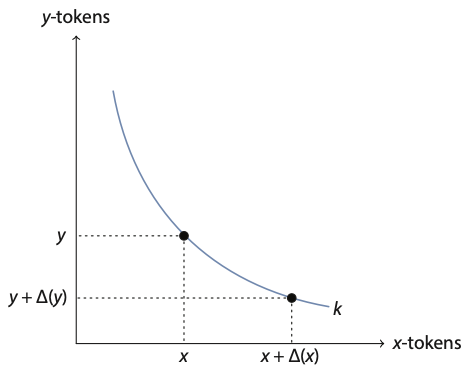
\includegraphics[width=0.5\textwidth]{background/Images/constant_product_formula.png}
    \caption{Constant Product Formula~\cite{schar2021decentralized}}
\end{figure}

\subsubsection{Slippage}

As seen in Figure \ref{fig:uniswap_lp}, we can see how the constant product formula is used in Uniswap. Uniswap also allow users to set slippage tolerance levels, which determine the maximum acceptable difference between the expected and executed prices. Slippage refers to the difference between the expected price of a trade and the executed price due to market volatility and liquidity conditions. Slippage happens because the constant product formula adjusts prices based on the ratio of tokens in the pool. As trades are executed, the token balances change, and the prices change accordingly. Thus, larger trades can cause more significant price impact, resulting in slippage.

\begin{figure}[!htb]
    \centering
    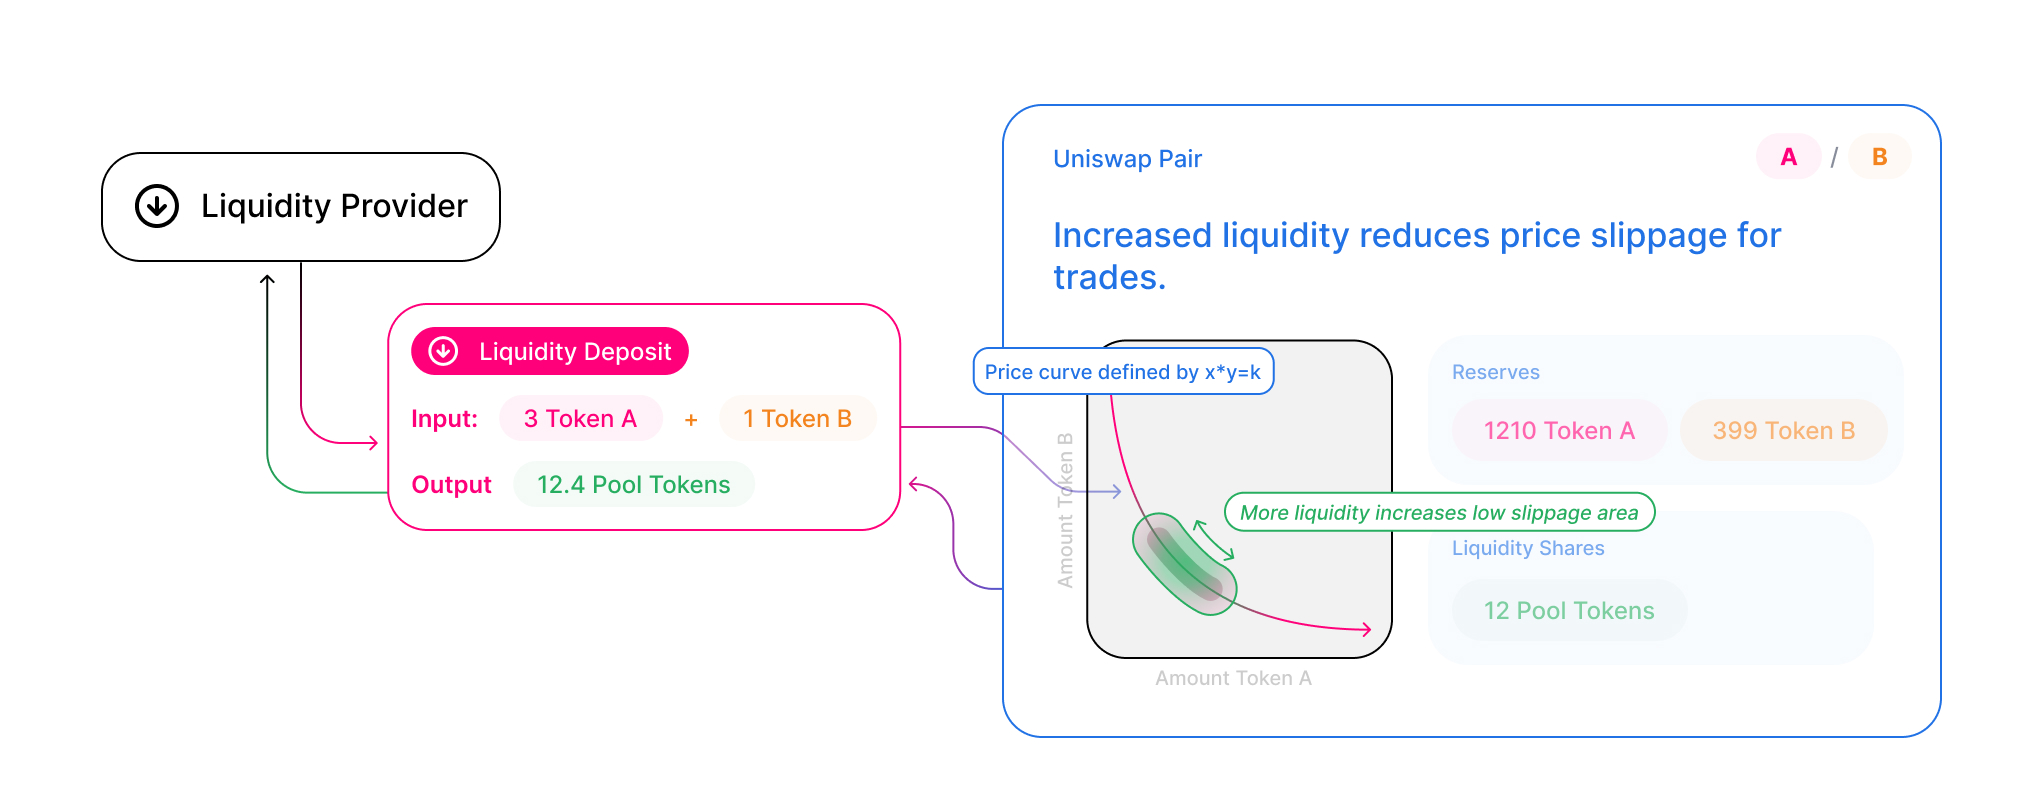
\includegraphics[width=\textwidth]{background/Images/uniswap_lp.jpeg}
    \caption{How Uniswap works~\cite{uniswap} \label{fig:uniswap_lp}}
\end{figure}

\subsection{Aave}

\subsubsection{Overview}
Aave is a decentralized lending and borrowing protocol built on the Ethereum blockchain. It enables users to lend and borrow a wide range of cryptocurrencies directly, without the need for intermediaries such as banks. Aave operates through liquidity pools and smart contracts, providing a secure, transparent, and efficient platform for decentralized finance (DeFi) activities.

Users can deposit their cryptocurrency assets into Aave's liquidity pools and earn interest on their deposits. These funds contribute to the available liquidity for borrowers. On the other hand, borrowers can use their deposited assets as collateral to borrow other assets from the pool. The amount they can borrow is determined by the value of their collateral and specific borrowing parameters set by the protocol.

\section{Fees that are incurred when trading}
As previously mentioned, when engaging in trading activities, there are several fees that are deducted. These fees serve multiple purposes, including compensating the liquidity providers and addressing the potential lack of access to assets from the lender. Therefore, in this section, we will delve into the various costs associated with implementing and executing the strategy.

\subsection{Gas Fees}
Gas fees in Ethereum are a crucial component of the network's operation. They serve two main purposes: to prevent spam and denial-of-service attacks and to incentivize miners to include transactions in the blockchain. They are a measure of computational effort required to execute a transaction or perform a smart contract operation on the Ethereum network. Each operation, such as sending tokens, executing a smart contract function, or interacting with decentralized applications, consumes a certain amount of gas.
\\[5mm]
The fee is calculated by multiplying the gas price (expressed in Gwei, where 1 Gwei is equal to 0.000000001 ETH) by the gas used~\cite{noauthor_gas_nodate}. As mentioned in previous sections, when a transaction is initiated by a user, the user specifies the gas limit which defines the maximum amount of gas that a user is willing to pay for a transaction, if the gas limit is too low and the gas used is greater than its limit, the transaction will fail and be reverted. This means that the state changes made by the transaction will not be recorded on Ethereum, and the fees paid for that transaction will be lost.

\begin{figure}[!htb]
    \centering
    \makebox[\textwidth]{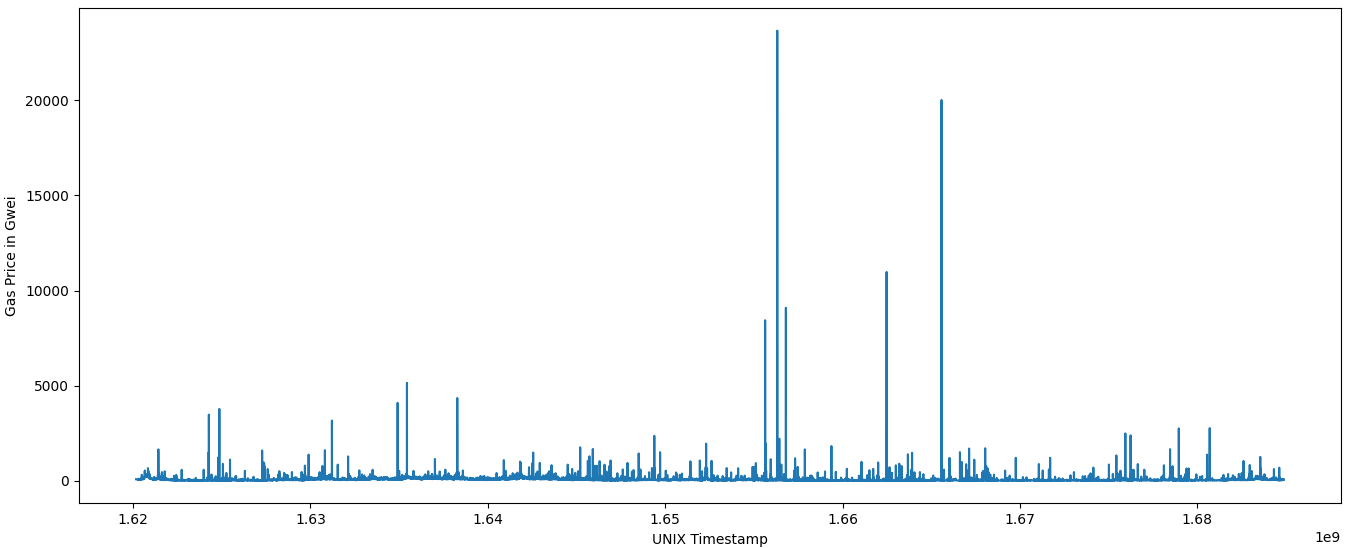
\includegraphics[width=1.15\textwidth]{project/Images/gas_price_1.png}}
    \caption{The gas price over time}
    \label{fig:gwei_over_time}
\end{figure}

\noindent Figure \ref{fig:gwei_over_time} the gas price history over time, showing the price surges and trophs. The reason for these fluctuations that it is determined by the market forces of supply and demand. It is the amount of Ether (ETH) that a user is willing to pay for each unit of gas consumed in a transaction. Miners have the option to prioritize transactions with higher gas prices, and thus are incentivized to include transactions with higher gas prices because they receive the gas fees as a reward for their mining efforts. Therefore, setting a higher gas price increases the chances of a transaction being executed.
\\[5mm]
The second part of the gas fee is how much gas is used, it is calculated by multiplying the gas cost of each operation in the transaction by the corresponding gas price. Each operation has a predefined gas cost associated with it, which reflects the complexity and resource requirements of that operation. When a transaction or smart contract execution is initiated, the Ethereum Virtual Machine (EVM) processes each operation and deducts the corresponding gas cost from the gas limit. In addition to this, Ethereum also has a base fee with all of their transactions thus having multiple small transaction becomes more costly than using a large combined transaction~\cite{noauthor_gas_nodate}.

\subsection{Uniswap Fees}
In addition to transaction fees, there is another fee mechanism in place within the system when swapping on Uniswap. This fee is designed to incentivize and reward liquidity providers on the platform. When a swap occurs, a fee is deducted from the amount of tokens expected to be returned to the user.
\\[5mm]
The fee is calculated as a percentage of the swap volume, meaning that the larger the swap, the higher the fee. For example, let's consider a scenario where the exchange price is 1 TKNA = 100 TKNB and the fee is set at 0.3\%. If someone exchanges 1 TKNA for TKNB, instead of receiving the full 100 TKNB based on the exchange rate, they will receive 100$\times$(1 - 0.3\%) TKNB = 99.7 TKNB. The fee reduces the total amount of tokens received in the swap.
\\[5mm]
It's important to note that the specific fee percentage may vary between different liquidity pools on Uniswap. Each liquidity pool can have its own fee tier, and the fees associated with each interested liquidity pools can be seen in Table \ref{tab:uniswap-fees}.

\begin{table}[!htb]
    \begin{tabular}{|l|l|l|r|}
        \hline
                                      Pool Address & Token0 & Token1 &  Fee Tier as a \% \\\hline\hline
        0x88e6a0c2ddd26feeb64f039a2c41296fcb3f5640 &   USDC &   WETH &     0.05 \\\hline
        0x8ad599c3a0ff1de082011efddc58f1908eb6e6d8 &   USDC &   WETH &     0.30 \\\hline
        0x11b815efb8f581194ae79006d24e0d814b7697f6 &   WETH &   USDT &     0.05 \\\hline
        0x4e68ccd3e89f51c3074ca5072bbac773960dfa36 &   WETH &   USDT &     0.30 \\\hline
        0x60594a405d53811d3bc4766596efd80fd545a270 &    DAI &   WETH &     0.05 \\\hline
        0xc2e9f25be6257c210d7adf0d4cd6e3e881ba25f8 &    DAI &   WETH &     0.30 \\\hline
        0xe0554a476a092703abdb3ef35c80e0d76d32939f &   USDC &   WETH &     0.01 \\\hline
        0xc5af84701f98fa483ece78af83f11b6c38aca71d &   WETH &   USDT &     0.1  \\\hline
    \end{tabular}
    \caption{Uniswap fees for each liquidity pool of interest \label{tab:uniswap-fees}}
\end{table}

\subsection{Aave Fees \& Collatoral}
Aave facilitates lending and borrowing transactions among users, and as part of its operations and incentive mechanisms, it imposes certain fees. In the context of this trading strategy, the only fees applicable would be the interest rates on the loan. The interest rate is typically expressed as an Annual Percentage Yield (APY) and is accrued continuously. Currently, Aave supports variable interest rates, which fluctuate based on market conditions, the borrowed asset, and supply and demand dynamics within the Aave.
\\[5mm]
Another aspect of Aave for the trading strategy is collateralization and the avoidance of liquidation. Liquidation occurs when a borrower's position is forcibly closed, and their collateral assets are sold off in cases of default or insufficient collateral. When borrowing from Aave, borrowers are required to allocate a certain percentage of the loan value as collateral, known as the Loan-to-Value (LTV) ratio~\cite{aave_risk}. For instance, if a token has a 75\% LTV, borrowers can borrow 0.75 ETH worth of the corresponding token for every 1 ETH worth of collateral provided. However, as token prices fluctuate, the ratio between the borrowed token value and the collateral value changes, posing risks for both lenders and Aave. To safeguard lenders and maintain protocol solvency, a liquidation threshold is established. If the collateral value falls below this threshold, the borrower's position becomes vulnerable to liquidation. In such cases, the collateral is auctioned off to repay the outstanding debt to the lenders. Typically, the liquidation threshold is set 5-10\% higher than the asset's LTV. For WETH, the Loan-to-Value ratio is 82.5\%, and the liquidation threshold is 86\%.


\subsubsection{Liquidity Pools}

The fundamental mechanism that enables Aave's functionality of lending and borrowing is liquidity pools. Users deposit their cryptocurrency assets into Aave's liquidity pools. These assets serve as collateral and contribute to the overall liquidity of the protocol. The deposited assets in the liquidity pools create reserves of available liquidity. These reserves are utilized to fulfill borrowing demands from other users within the Aave ecosystem.

\subsubsection{Lending and Borrowing}

Lending works by lenders depositing their cryptocurrency assets into Aave's liquidity pools. These assets act as collateral and are represented by interest-bearing tokens called aTokens. The aTokens represent the user's share of the deposited assets. Interest is earnt immediately and is accrued in real-time and reflected in an increase in the quantity of aTokens held by the depositor.

Borrowing works by borrowers using their deposited assets as collateral to borrow other assets from the liquidity pools. The value of the collateral determines the borrowing capacity. The borrowing capacity is calculated by paramters set by Aave, one of which is the maximum loan-to-value (LTV) ratio. Once the borrower requests a loan, if the borrower's collateral meets the necessary requirements, they can proceed with the loan and the borrowed funds are transferred to the borrower's wallet. In addition to this, borrowers pay interest on the borrowed amount based on the prevailing interest rates. Aave offers both variable and stable interest rates for borrowers. Variable rates fluctuate based on market dynamics, while stable rates remain fixed. This flexibility allows users to choose the borrowing option that best suits their needs. The interest on a loan is accrued in real-time, second by second, and the borrower decides when to repay it, as long as the loan is safe from liquidation. Liquidation is what happens if the value of a borrower's collateral falls below the liquidation threshold due to market volatility or other factors, the collateral may be liquidated. Liquidators can purchase the collateral at a discounted price to ensure the solvency of the liquidity pool.

\section{Liquidity Pool Pairs of Interest}
\label{sec:liquidity-pools}
As previously mentioned, Uniswap is a decentralized exchange protocol that facilitates swapping of cryptocurrencies through the use of liquidity pools. One of the remarkable features of Uniswap is its support for even the smallest cryptocurrencies. In fact, it currently possesses 12,182 liquidity pools, as obtained via the Uniswap V3 subgraph. The subgraph provides valuable insights into the liquidity pools within the Uniswap ecosystem.
\\[5mm]
Table \ref{tab:liquidity_pools} showcases the diversity of these pools. Some pools exhibit high trading volumes, indicating significant activity and demand for those specific pairs. On the other hand, there are also pools with zero liquidity, which could be attributed to various reasons. It could be due to a lack of demand for one of the token pairs offered in the pool, or it may indicate that the pool is relatively new and has not attracted significant participation yet.
\\[5mm]
To enhance the chances of successful swaps and maximize potential profitability, my strategy is centered on liquidity pools with a trading volume surpassing \$10,000,000 (or \$10 million) and pools that include tokens supported by Aave. Additionally, I exclude any liquidity pools that do not involve WETH, which is a tokenized form of ETH (Ethereum's native cryptocurrency). WETH's key advantage lies in its ability to align with ERC-20 standards, enabling broader compatibility and utilization across the Ethereum ecosystem.

\begin{table}[!ht]
    \centering
    \begin{tabular}{|p{7em}|p{4em}|p{4em}|p{10em}|p{\linewidth / 6}|p{4em}|}
    \hline
        pool address & token0 & token1 & volume in USD & created at timestamp & feetier \\ \hline
        \truncate{7em}{0x88e6a0c2ddd26feeb64f039a2c41296fcb3f5640} & USDC & WETH & \truncate{10em}{375230561243.465} & 1620250931 & 500 \\ \hline
        \truncate{7em}{0x8ad599c3a0ff1de082011efddc58f1908eb6e6d8} & USDC & WETH & \truncate{10em}{70454095868.0967} & 1620169800 & 3000 \\ \hline
        \truncate{7em}{0x11b815efb8f581194ae79006d24e0d814b7697f6} & WETH & USDT & \truncate{10em}{62385006691.8387} & 1620251172 & 500 \\ \hline
        \truncate{7em}{0x3416cf6c708da44db2624d63ea0aaef7113527c6} & USDC & USDT & \truncate{10em}{57192593471.8346} & 1636825557 & 100 \\ \hline
        \truncate{7em}{0x4585fe77225b41b697c938b018e2ac67ac5a20c0} & WBTC & WETH & \truncate{10em}{49170385539.9928} & 1620246230 & 500 \\ \hline
        \truncate{7em}{0x4e68ccd3e89f51c3074ca5072bbac773960dfa36} & WETH & USDT & \truncate{10em}{30135014933.0963} & 1620232628 & 3000 \\ \hline
        \truncate{7em}{0x60594a405d53811d3bc4766596efd80fd545a270} & DAI & WETH & \truncate{10em}{26075053939.434} & 1620237823 & 500 \\ \hline
        \truncate{7em}{0xcbcdf9626bc03e24f779434178a73a0b4bad62ed} & WBTC & WETH & \truncate{10em}{21870989841.1326} & 1620158974 & 3000 \\ \hline
        \truncate{7em}{0x5777d92f208679db4b9778590fa3cab3ac9e2168} & DAI & USDC & \truncate{10em}{16143305036.8948} & 1636771503 & 100 \\ \hline
        \truncate{7em}{0x7858e59e0c01ea06df3af3d20ac7b0003275d4bf} & USDC & USDT & \truncate{10em}{15473402409.0591} & 1620159478 & 500 \\ \hline
        \truncate{7em}{0x99ac8ca7087fa4a2a1fb6357269965a2014abc35} & WBTC & USDC & \truncate{10em}{12568187132.1649} & 1620241995 & 3000 \\ \hline
        \truncate{7em}{0xc2e9f25be6257c210d7adf0d4cd6e3e881ba25f8} & DAI & WETH & \truncate{10em}{12519316091.9979} & 1620159368 & 3000 \\ \hline
        \truncate{7em}{0xe0554a476a092703abdb3ef35c80e0d76d32939f} & USDC & WETH & \truncate{10em}{9381529300.20357} & 1636926269 & 100 \\ \hline
        \truncate{7em}{0x6c6bc977e13df9b0de53b251522280bb72383700} & DAI & USDC & \truncate{10em}{7219493916.70291} & 1620158293 & 500 \\ \hline
        \truncate{7em}{0xac4b3dacb91461209ae9d41ec517c2b9cb1b7daf} & APE & WETH & \truncate{10em}{6621032721.87519} & 1647516735 & 3000 \\ \hline
        \truncate{7em}{0x8c54aa2a32a779e6f6fbea568ad85a19e0109c26} & FEI & USDC & \truncate{10em}{6206853090.73714} & 1621839430 & 500 \\ \hline\hline
        \truncate{7em}{0x53dd58b3143f428b449c16dd5706cee7d7bcf408} & sOHM & gOHM & 0 & 1652914688 & 10000 \\ \hline
        \truncate{7em}{0xbc90c4de85a4b559060cb28abfd4476ab6711f1a} & SHIB & NSTIC & 0 & 1652910391 & 100 \\ \hline
        \truncate{7em}{0xaa1297b08d0035f06309c1bfa36582c24b4ae361} & BUSD & DPC & 0 & 1674655715 & 100 \\ \hline
        \truncate{7em}{0x75087e5330c97f7ec7f716c6566f214cb0029f6a} & DAI & ICAP & 0 & 1652899566 & 10000 \\ \hline
        \truncate{7em}{0xc65a680191bd17a18c957c8aa2d1155ed2322792} & stkAAVE & FRAX & 0 & 1652817927 & 10000 \\ \hline
        \truncate{7em}{0x94589b18b95b355ee9a900f3df671b431779e20a} & VVV & SOL & 0 & 1674701603 & 10000 \\ \hline
        \truncate{7em}{0xf42f0def92337b6a83753c9fae6d579f7d67aaa9} & APEFI & ApeUSD & 0 & 1652808878 & 3000 \\ \hline
        \truncate{7em}{0xb9ba65f1568b318ffc1879a4a6368ef2b5ac96b8} & FRAX & ApeUSD & 0 & 1652808680 & 500 \\ \hline
        \truncate{7em}{0x1dfb167f1ba47f3bf835eb60a9317b4601925642} & GHD & WETH & 0 & 1652784327 & 3000 \\ \hline
    \end{tabular}
    \caption{A selection of liquidity pools on Uniswap \label{tab:liquidity_pools}}
\end{table}

\subsection{Correlated and Cointegrated Liquidity Pools}
Once the liquidity pools of interested in have been identified, it is crucial to filter the pool pairs based on their correlation. This is because correlated pairs tend to exhibit similar pricing movements thus would be possible to apply the mean reversion trading strategies. However, it is important to strike a balance between a highly correlated pair and a low correlated pair, as excessively high correlation can result in minimal price deviations, leading to fees that exceed the deviations and resulting in overall losses instead of profits. To address this, I have set a condition where the correlation coefficient ($\rho$) should fall within the range of $0.992 \leq \rho \leq 0.997$. Figure \ref{fig:correlationMatrix} shows the correlation matrix of the liquidity pools that meet the initial requirement of having a volume greater than \$10 million volume ratio and include WETH. Notably, the pools associated with tokens aiming to be pegged to the US Dollar, such as USDT, USDC, and DAI, exhibit the expected high correlation with each other. However, an exception is observed with pool 0xe0554a476a092703abdb3ef35c80e0d76d32939f, which exhibits a lower correlation with other liquidity pools containing these stable coins. Consequently, this lower correlation opens up additional avenues for potential arbitrage opportunities within the pool.
\begin{figure}[!htb]
    \centering
    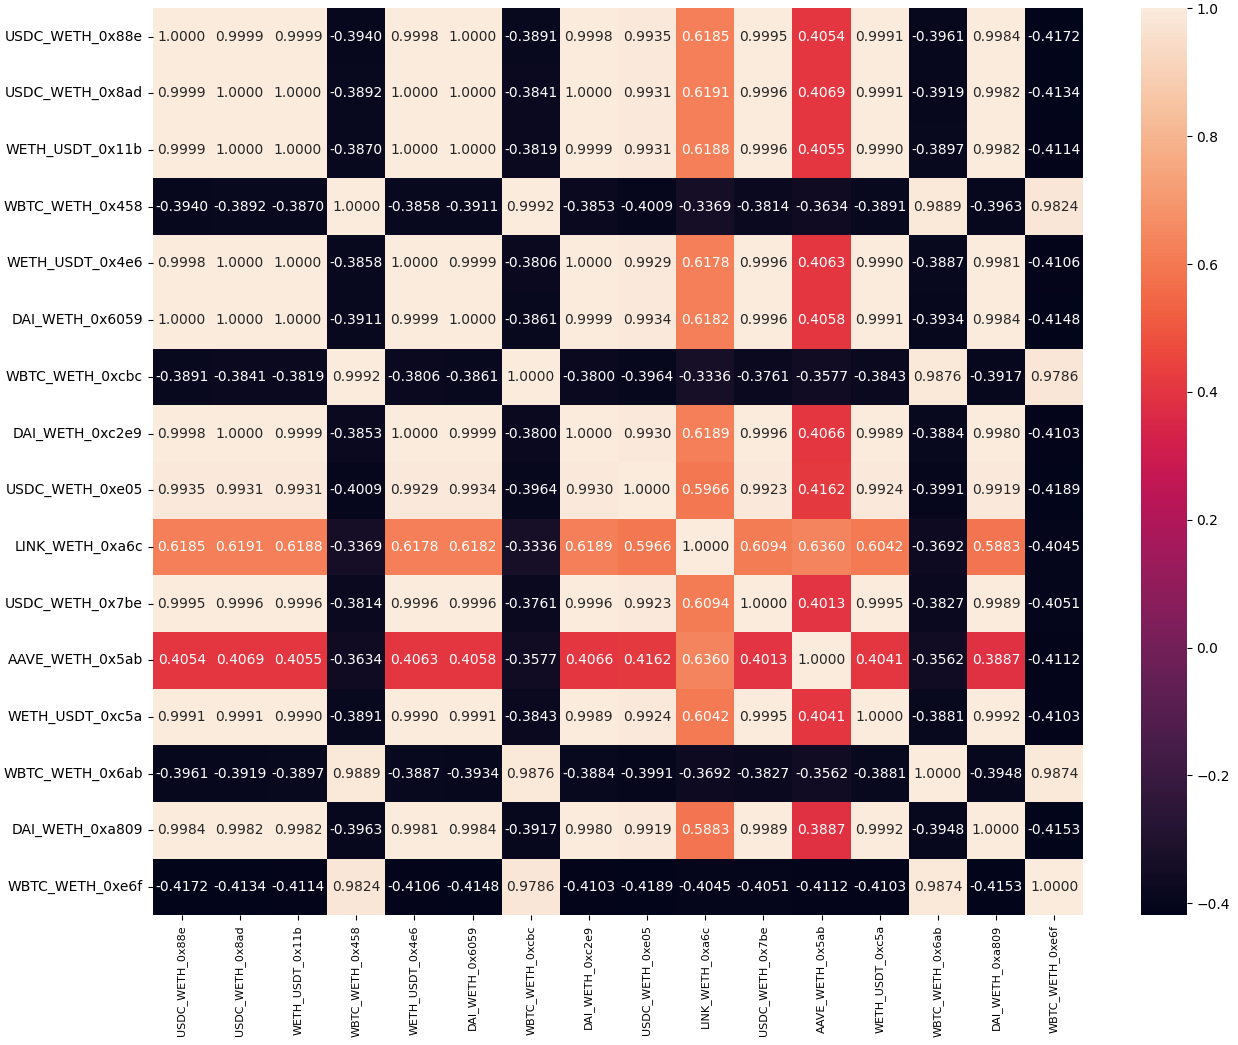
\includegraphics[width=\textwidth]{project/Images/correlationMatrix.png}
    \caption{Correlation Matrix of the Liquidity Pools that meet the \$10 million volume and include WETH \label{fig:correlationMatrix}}
\end{figure}
\\[5mm]
To determine which liquidity pools are cointegrated, I employed the Engle-Granger approach. The Engle-Granger test for cointegration involves several steps. Firstly, a unit root test is performed individually on each time series using methods like the Augmented Dickey-Fuller (ADF) test or the Phillips-Perron (PP) test. These tests assess whether the time series are stationary or exhibit unit roots (non-stationary) individually. For cointegration to hold, both time series must be non-stationary.
\\[5mm]
Once it is established that both time series are non-stationary, an estimation of the cointegration equation is derived. Typically, a linear regression model is employed to capture the long-term relationship between the time series variables. This equation provides an understanding of how the variables are linked over a long period.
\\[5mm]
Subsequently, a unit root test is conducted on the residuals obtained from the regression analysis. If the residuals are stationary (indicating the absence of unit roots), it suggests the presence of cointegration between the time series. This implies that the variables move together in the long run, even if short-term deviations occur.
\\[5mm]
By following the aforementioned sequence of steps in the Engle-Granger test, it enables us to determine which liquidity pools demonstrate cointegration, thereby emphasizing their interconnectedness and mutual relationship over time. The outcome of the cointegration tests for all possible combinations of liquidity pools is presented in Table \ref{tab:coin_pools}. This table provides a comprehensive list of the liquidity pool pairs along with the results of their respective cointegration tests and the correlation coefficient of each combination.
\begin{table}[!ht]
    \centering
    \begin{adjustwidth}{-1in}{-0.9in}
        \begin{tabular}{|p{12em}|p{12em}|p{5em}|p{4.2em}|p{4.2em}|p{4.2em}|p{3.5em}|}\hline
            pool1 & pool2 & t-statistic of unit-root test on residuals & \multicolumn{3}{|c|}{Critical Values} & Corr Coeff\\[-1ex]\cline{4-6}
            &   &   & 1\% & 5\% & 10\% & \\\hline
            \truncate{12em}{USDC\_WETH\_0x88e6a0c2ddd26feeb64f039a2c41296fcb3f5640} & \truncate{12em}{USDC\_WETH\_0xe0554a476a092703abdb3ef35c80e0d76d32939f} & -11.306176 & -3.898069 & -3.337038 & -3.045081 & 0.99347\\\hline
            \truncate{12em}{USDC\_WETH\_0x8ad599c3a0ff1de082011efddc58f1908eb6e6d8} & \truncate{12em}{USDC\_WETH\_0xe0554a476a092703abdb3ef35c80e0d76d32939f} & -11.210146 & -3.898082 & -3.337046 & -3.045086 & 0.99307\\\hline
            \truncate{12em}{WETH\_USDT\_0x11b815efb8f581194ae79006d24e0d814b7697f6} & \truncate{12em}{USDC\_WETH\_0xe0554a476a092703abdb3ef35c80e0d76d32939f} & -10.010746 & -3.898069 & -3.337038 & -3.045081 & 0.99315\\\hline
            \truncate{12em}{WETH\_USDT\_0x4e68ccd3e89f51c3074ca5072bbac773960dfa36} & \truncate{12em}{USDC\_WETH\_0xe0554a476a092703abdb3ef35c80e0d76d32939f} & -9.913205 & -3.898081 & -3.337045 & -3.045085 & 0.99291\\\hline
            \truncate{12em}{DAI\_WETH\_0x60594a405d53811d3bc4766596efd80fd545a270} & \truncate{12em}{USDC\_WETH\_0xe0554a476a092703abdb3ef35c80e0d76d32939f} & -11.395276 & -3.898069 & -3.337038 & -3.045081 & 0.99338\\\hline
            \truncate{12em}{DAI\_WETH\_0xc2e9f25be6257c210d7adf0d4cd6e3e881ba25f8} & \truncate{12em}{USDC\_WETH\_0xe0554a476a092703abdb3ef35c80e0d76d32939f} & -10.418722 & -3.89831 & -3.337173 & -3.045174 & 0.99298\\\hline
            \truncate{12em}{USDC\_WETH\_0xe0554a476a092703abdb3ef35c80e0d76d32939f} & \truncate{12em}{WETH\_USDT\_0xc5af84701f98fa483ece78af83f11b6c38aca71d} & -9.7789 & -3.901414 & -3.338902 & -3.046374 & 0.99243\\\hline
        \end{tabular}
    \end{adjustwidth}
    \caption{Cointegration test on Liquidity Pool pairs \label{tab:coin_pools}}
\end{table}
\\[5mm]
\noindent Based on the results obtained, we focus our further investigation solely on the pairs of liquidity pools that exhibit cointegration under a 1\% confidence level. This filtering process allows us to narrow down our analysis to those pairs where a long-term relationship exists, suggesting that they move together in a concerted manner.
\\[5mm]
By concentrating on the cointegrated pairs, we can delve deeper into exploring their dynamics, assessing their behavior, and leverage the interconnectedness between these liquidity pools. This approach enables us to prioritize our analysis and concentrate on the most relevant liquidity pool combinations that offer potential opportunities for profitable trading or other related activities.




\chapter{Implementation of the Trading Systems}
This section provides a comprehensive overview of the two trading system implementations. The first focuses on the backtesting system, which simulates and evaluates strategies in a controlled environment. In this system, historical market data is utilised to test and analyse the performance of various strategies. The second implementation is the live system, designed to execute trades on the Ethereum blockchain using smart contracts. This system operates in real time and interacts with the live market, allowing actual trades to be executed based on predefined strategies. Together, these two implementations provide a comprehensive framework for testing, evaluating, and deploying trading strategies in simulated environments and on the live blockchain.

\section{Backtesting System}
\label{sec:backtesting-sys}

To develop a resilient backtesting system, a dedicated class was constructed to streamline the process of testing trading strategies; the system is entirely written in Python as it possesses countless libraries, including Pandas and Numpy, which are extensively used for data manipulation and analysis, it also is good with integrating with many data sources such as GraphQL which is required for this project. To evaluate a particular strategy, the \texttt{backtest} function requires \texttt{cointegrated\_pair}, a tuple of the names of the liquidity pools that the strategy is to be evaluated on, \texttt{strategy}, the strategy, and finally, the \texttt{initial\_investment} in ETH. The first argument is required and used to retrieve the relevant historical prices. The second parameter is self-explanatory, the strategy to test. Finally, including the initial investment amount as an input parameter enables users to simulate the performance of their strategies with a specific starting capital; it also helps analyse how the various transaction costs affect the ability to trade if any trades result in a loss. The \texttt{backtest} function iterates through historical data calling the strategy's \texttt{generate\_signal} and executing the trade orders it receives at each timestep. However, historical data is required; hence, the first step is to collect the historical data. The logical process of backtesting a pair can be seen in Figure \ref{fig:backtesting-flow}.
\begin{figure}[H]
    \centering
    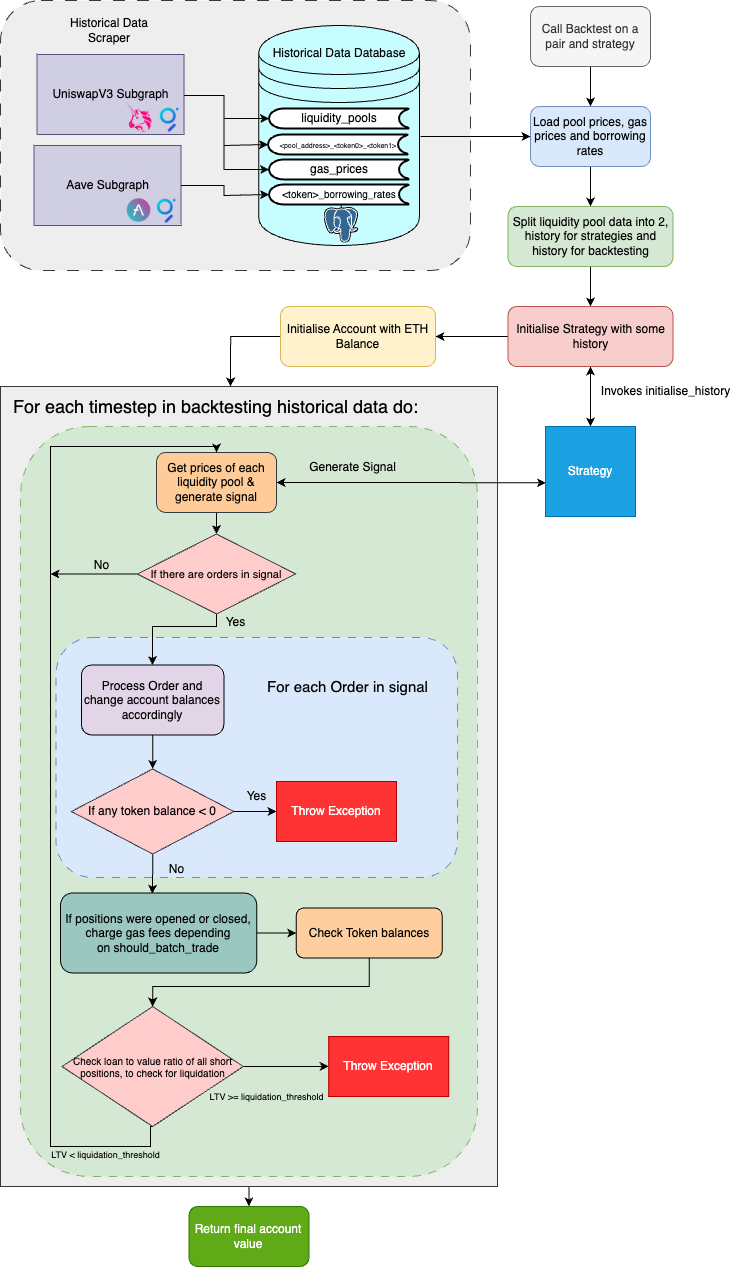
\includegraphics[width=0.99\textwidth]{project/Images/backtesting-diagram.png}
    \caption{Flowchart of backtesting a strategy on a liquidity pool pair \label{fig:backtesting-flow}}
\end{figure}

\subsection{Data Collection and Storage}
In order to simulate the market as accurately as possible, the system should have access to reliable and accurate historical market data, including price, volume, and other relevant indicators. Therefore, all of the data is retrieved from the Uniswap and Aave protocols' subgraph using the Graph~\cite{noauthor_graph_nodate}. The Graph is a decentralised protocol for indexing and querying blockchain data, making the data provided 100\% reliable as it indexes directly on the Ethereum blockchain. Subgraphs are GraphQL APIs designed to facilitate querying and extracting data from the blockchain. These APIs adhere to a specific schema outlined by the protocol, enabling seamless communication between the protocol and the underlying blockchain. Therefore, the Uniswap V3, Aave V2, and Aave V3 subgraphs are used to obtain the data required for the backtesting system.
\\[3mm]
In order to store the necessary data for backtesting and trading, a PostgreSQL database is used to provide consistency and flexibility, supporting numerous data types and a large set of SQL functions that allow for advanced querying. The database adopts the following schema:
\begin{figure}[!htb]
    \centering
    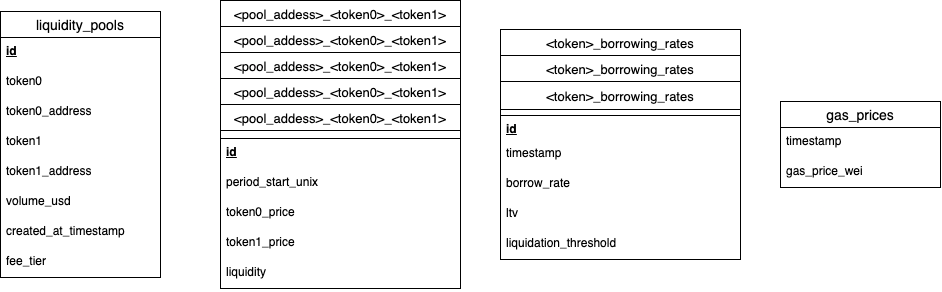
\includegraphics[width=0.8\textwidth]{project/Images/database_tables.png}
    \caption{Tables contained in the database \label{fig:database}}
\end{figure}
\\[3mm]
The \texttt{liquidity\_pools} contains data about the liquidity pools on Uniswap V3. After obtaining all of the data, it is found that it possesses 12,182 liquidity pools. However, most of these pools exhibit minimal or negligible trading volume. As a result, a criterion is established to selectively include only those liquidity pools that involve tokens supported by Aave and possess a trading volume exceeding \$10,000,000 (or \$10 million). This filtering condition ensures that the collected and stored data holds significance and relevance for research purposes, as these pools would allow for short selling.
\\[3mm]
Once these pools have been identified, pricing data about each pool that meets this condition is collected again using the Uniswap V3 subgraph. The query returns an array of dictionaries containing the pre-specified pricing data points at a frequency of every hour. Due to the limitations imposed by the subgraph, the results are constrained to a maximum size of 1000 entries. Hence, the query is executed iteratively to overcome this limitation and obtain the complete dataset. The previous maximum time, referred to as \texttt{prev\_max\_time}, is passed as an argument in subsequent queries to fetch the remaining data, i.e. \texttt{prev\_max\_time = hourlyData[-1]['periodStartUnix'] if len(hourlyData) > 0 else prev\_max\_time}. This data is stored in tables of the form \textit{<pool\_address>}\_\textit{<token0>}\_\textit{<token1>}.
\\[3mm]
Similarly, obtaining the interest rates for borrowing necessitates the utilisation of two of Aave's subgraphs. This requirement arises due to Aave's migration to Version 3 in March 2022, resulting in a transitional period where Uniswap V3 and Aave V2 were concurrently utilised. The schemas for the two are different; however, for the data we require, the borrowing rate, loan-to-value and liquidity threshold, the schema is consistent, and the same query can be used; this can be seen in Appendix \ref{app:lending-query}. During the table initialisation process, requests are made to the V2 and V3 GraphQL endpoints. However, only the V3 endpoint is utilised for sending requests when updating the table. The data is stored in tables of the form \textit{<symbol>}\_borrowing\_rates, where \textit{<symbol>} are all of the tokens that are present in the liquidity pools that are of interest.
\\[3mm]
The transaction history is queried at each hour to collect the gas price history since Uniswap migrated to V3. This is because querying in the same as the pricing data and borrowing rate history is too exhaustive as transactions occur every second. Therefore, it is more efficient to query at each hour with a window to retrieve the gas price at the closest hour as follows. Algorithm \ref{alg_gas_price_col} in the Appendix shows the pseudocode gas price at each hour is queried. 
\subsection{Types of Orders and Execution}
There are numerous order types that the backtesting supports due to measures to ensure a positive balance and avoid liquidation. The types of orders are; \texttt{BUY\ ETH}, \texttt{WITHDRAW}, \texttt{DEPOSIT}, \texttt{SWAP}, \texttt{OPEN\ BUY}, \texttt{CLOSE\ BUY}, \texttt{OPEN\ SELL}, \texttt{CLOSE\ SELL}. The procedures of each are outlined below. The code of the execution, excluding gas fees, of the order is outlined in Appendix \ref{sec:backtesting-execution-code}.

\subsubsection{\texttt{BUY\ ETH}}
The \texttt{BUY\ ETH} order is used to swap a percentage of the accounts balance of WETH to ETH. The argument is a float between 0 and 1.

\subsubsection{\texttt{SWAP}}
The \texttt{SWAP} order is to execute a simple swap for either token0 or token1 of the liquidity pool. This order is only used as a precautionary order if the balance of the WETH balance gets too low. It takes two arguments, the first indicating whether it is swapping for token0 or token1, and the second parameter is a list of swaps, tuples containing with pool and the quantity that would like to be swapped. The amount received in the account is multiplied by \texttt{(1 - swap\_fees[swap\_token])}, this is because Uniswap charges a percentage of the swap specified by \texttt{swap\_fees[swap\_token]}.

\subsubsection{\texttt{OPEN\ BUY}}
Similar to the \texttt{SWAP} order, \texttt{OPEN\ BUY} opens a buy position. As mentioned above, opening a buy order is simply swapping token1 for token0. The parameters of buying are the target token and the volume. 

\subsubsection{\texttt{CLOSE\ BUY}}
Closing a buy position is similar to opening a buy position; however, the swap is in the other direction, i.e. from token to WETH. The only argument is the id of the buy order. To account for Uniswap's fees, the volume received after the initial swap is calculated and then swapped back to WETH.

\subsubsection{\texttt{OPEN\ SELL}}
Opening a sell position involves borrowing a token and then swapping the token. The parameters of selling are the target token and the volume. It also consists of depositing the required amount to borrow the volume ordered, calculated by the value-to-loan ratio.

\subsubsection{\texttt{CLOSE\ SELL}}
Closing a sell position is more complicated; it requires swapping back from the token to WETH, repaying the loan with interest and finally returning collateral. Swapping back to the required amount of tokens is the first step. For this, the variable Annual Yield Rates between the timestamp of the opening and the closing position are used to calculate the amount of interest required to be paid, as this is cumulated every second. Once the volume of tokens required to be returned is calculated, the equivalent amount of WETH plus accounting for Uniswap fees is swapped to obtain these tokens. Finally, the tokens are repaid, and the collateral is returned.

\subsubsection{\texttt{WITHDRAW}}
The \texttt{WITHDRAW} order's function is to withdraw some collateral stored in Aave. It is not used in the strategies however is implemented in case of developing further strategies that may require this functionality. The only parameter is the amount that would like to be withdrawn.

\subsubsection{\texttt{DEPOSIT}}
The \texttt{DEPOSIT} order's function is to deposit some additional collateral stored in Aave. This order is used when the collateral value not properly covering the loan value, hence avoiding liquidation. The only parameter is the amount that would like to be deposited. 

\subsection{Gas Fees}
The remaining fee yet to be discussed is the gas fee for each order. To best approximate the gas fee, it is paramount to have an approximation of how much gas is used in each. Therefore, the smart contract for trading was written and run on a forked Ethereum mainnet to accurately simulate the contracts behaviour; see Subsection \ref{sec:smart-contracts} to see the implementation of the smart contract. Using Hardhat, the gas usage of each function was tested, and Figure \ref{fig:gasResult} shows the results. It can be seen that some functions have a tighter spread, between the maximum and minimum, compared to others; therefore, to better understand this, plots using various parameters on the different functions provided a deeper insight into the cause of this, Figures \ref{fig:gasPlots1} and \ref{fig:gasPlots2}.
\begin{figure}[!htb]
    \centering
    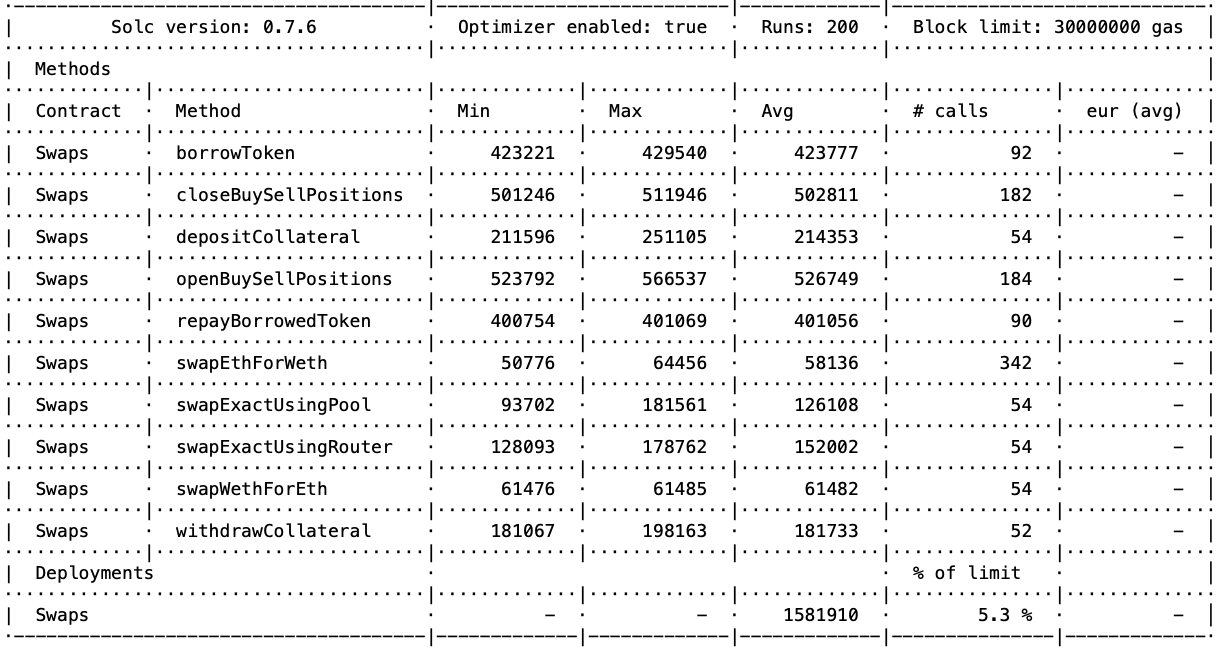
\includegraphics[width=0.9\textwidth]{project/Images/gas_fee_results.png}
    \caption{Results from running smart contract functions \label{fig:gasResult}}
\end{figure}

\begin{figure}[!htb]
    \centering
    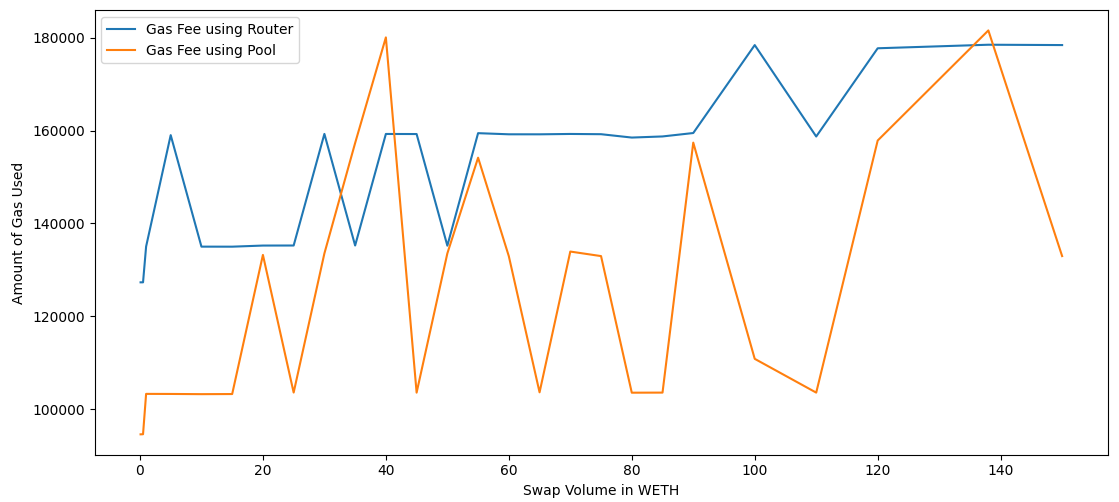
\includegraphics[width=0.9\textwidth]{project/Images/SwapFeesPlot.png}\\
    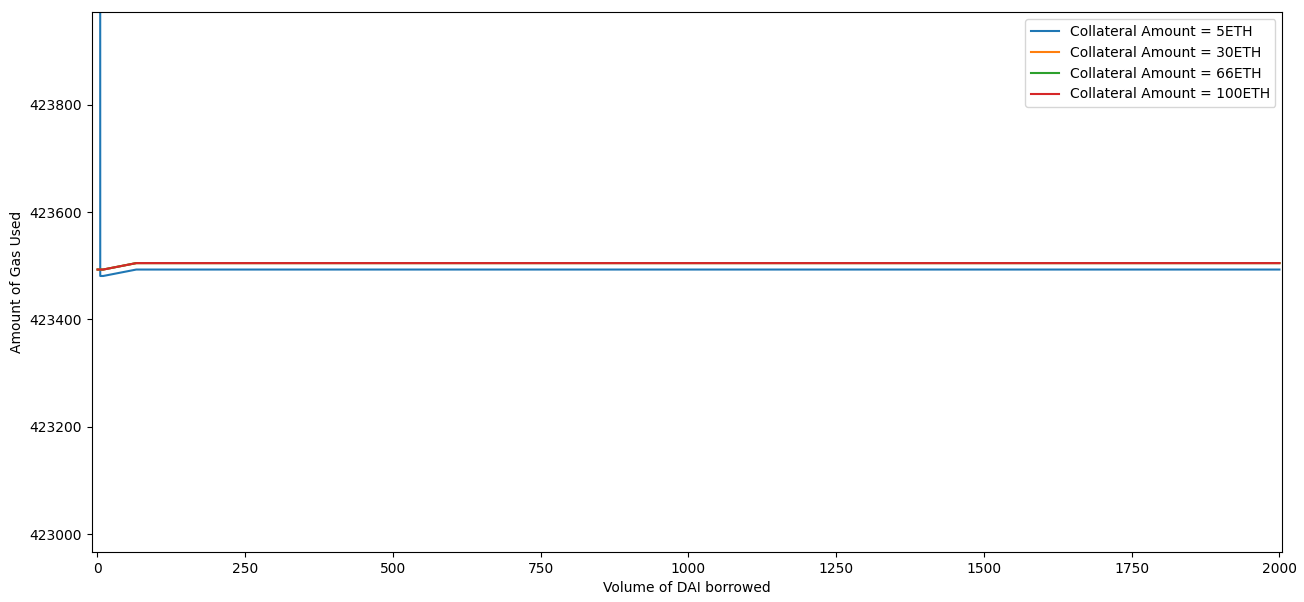
\includegraphics[width=0.9\textwidth]{project/Images/BorrowFees2.png}
    \caption{Gas Usage Plots of Gas Used by Swapping (Top) and Borrowing (Bottom) \label{fig:gasPlots1}}
\end{figure}

\begin{figure}[!htb]
    \centering
    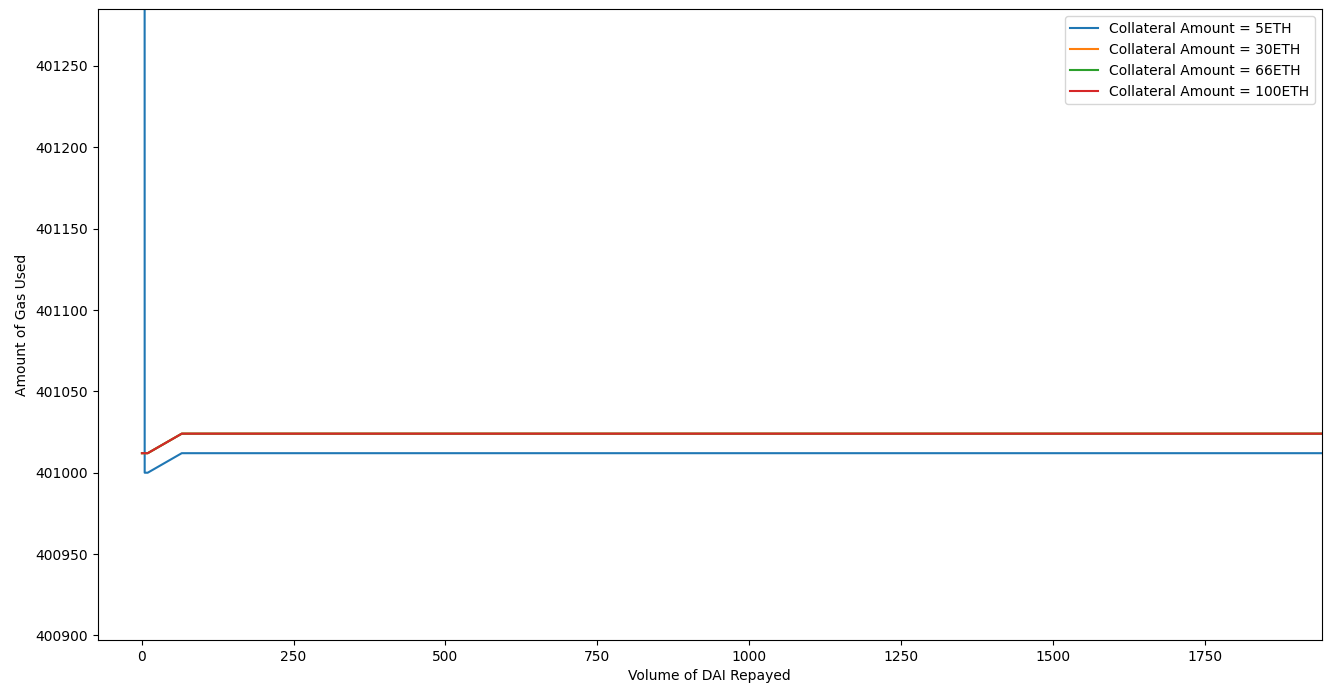
\includegraphics[width=0.9\textwidth]{project/Images/RepayFees2.png}\\
    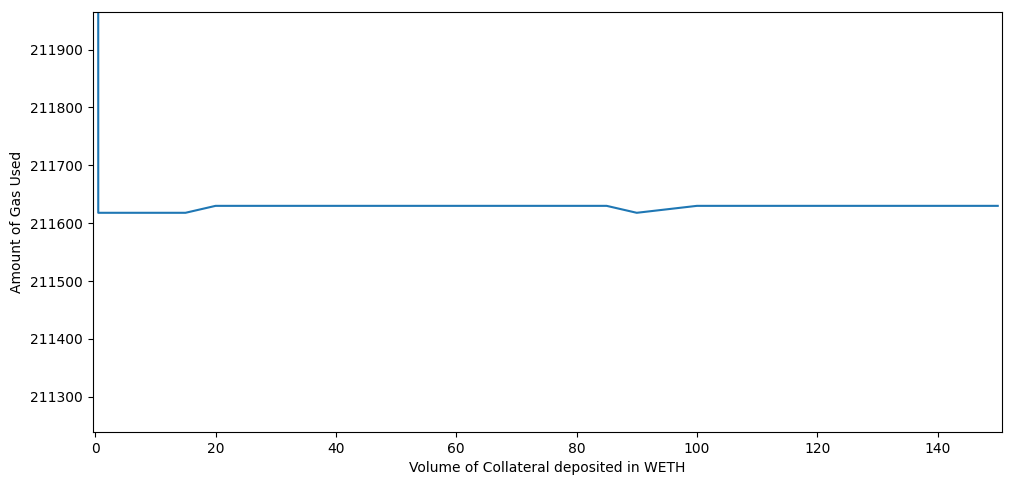
\includegraphics[width=0.9\textwidth]{project/Images/depositFeesPlot2.png}
    \caption{Gas Usage Plots of Gas Used by Repaying Borrowed Tokens (Top) and Depositing additional tokens (Bottom) \label{fig:gasPlots2}}
\end{figure}

\noindent Upon analysing these plots, it becomes apparent that the majority of the functions exhibit a high level of consistency. However, it is noteworthy that for the smallest quantity tested, the gas consumption is significantly higher than that of larger quantities. Nevertheless, once this threshold is surpassed, gas usage remains consistent. Therefore the average gas usage of each operation is used in the backtesting system as it provides a representative estimate of the gas consumption across different quantities.
\\[3mm]
Furthermore, another interesting feature is the gas usage by swaps and the different methods. The initial method utilises Uniswap's Router, which scans all available liquidity pools to identify the optimal price, whereas the second method involves direct swapping within a specific liquidity pool. Figure \ref{fig:gasPlots1} illustrates that, on average, the router-based approach exhibits higher gas usage than direct swapping using a liquidity pool. However, directly swapping using a liquidity pool exhibits greater volatility in gas consumption but also consistently returns to values above 100,000; because of this, the average gas usage of swapping using a liquidity pool is used.
\\[3mm]
It can also be seen that combining the operations to open/close buy and sell positions consumes less gas compared to if they were to be executed separately. This also confirms the claims in Wang's paper that batching the operations together is more effective than executing them separately~\cite {wang_cyclic_2022}. Thus incorporating this into the backtesting system, each order deducts some ETH, which is calculated by how much gas is used by the order type multiplied by the gas price. For example, in the case of buying more ETH:
\begin{lstlisting}[language=Python]
amount_to_swap = self.account['WETH'] * order[1]
self.account['WETH'] = self.account['WETH'] - amount_to_swap
self.account['ETH'] = self.account['ETH'] + amount_to_swap - (GAS_USED_BY_BUYING_ETH * gas_price_in_eth)
\end{lstlisting}
\vspace{5mm}
\noindent However, in order to analyse the impact of combining operations on strategy returns, the deduction of ETH for gas fees for both \texttt{OPEN} and \texttt{CLOSE} orders is handled differently. Instead of deducting the fees immediately upon each order, the deduction is performed after iterating through the trading signal. If the signal contains such orders, the necessary amount of gas fee is deducted based on whether the orders are specified, by the parameter \texttt{should\_batch\_trade}, to be batched or executed separately. The code for handling this can be seen in Appendix \ref{app:deducting-gas-fee}.

\subsection{Validating Balance Health}
To maintain the integrity and effectiveness of the trading strategy, it is crucial to incorporate various checks and safeguards after each trade and at each timestep. One key aspect involves monitoring the balance of each token to ensure that it remains positive. After every order execution, the tokens' balances are checked, and if any of them fall below zero, an exception is triggered.
\begin{lstlisting}[language=Python]
if self.account['T1'] < negative_threshold:
    raise Exception('Account balace goes below 0 - T1')
if self.account['T2'] < negative_threshold:
    raise Exception('Account balace goes below 0 - T2')
if self.account['WETH'] < negative_threshold:
    raise Exception('Account balace goes below 0 - WETH')
if self.account['ETH'] < negative_threshold:
    raise Exception('Account balace goes below 0 - ETH')
\end{lstlisting}   
Furthermore, the loan-to-value ratio is calculated to simulate the potential liquidation of a sell position's loan. This ratio serves as an indicator of the position's health and risk level. If the loan-to-value ratio breaches the predefined liquidation threshold, an exception is thrown, indicating that the position is approaching an unsustainable state.
\begin{lstlisting}[language=Python]
sell_token, sold_price, sell_volume, _ = sell_trade
current_token_price = prices[f'P{sell_token[1]}']
curr_value_of_loan_pct = (sell_volume * current_token_price) / self.account['collateral_WETH']
if round(curr_value_of_loan_pct, 4) > liquidation_threshold:
    raise Exception(f'Short position liquidated')
\end{lstlisting}

\section{Live Trading}
A similar approach is required to run the strategies live; however, the execution system and balance tracking are altered. For the system, multiple components are required for live trading to occur. The first is the ability to interact with the blockchain to execute the orders; handled by smart contracts; the second is to manage the state of the strategy, accounts and open positions for the strategies to use to generate signals, and finally, a method to convert the signal into smart contract invocations to execute the orders—the workflow of trading on the live execution system.
\begin{figure}[H]
    \centering
    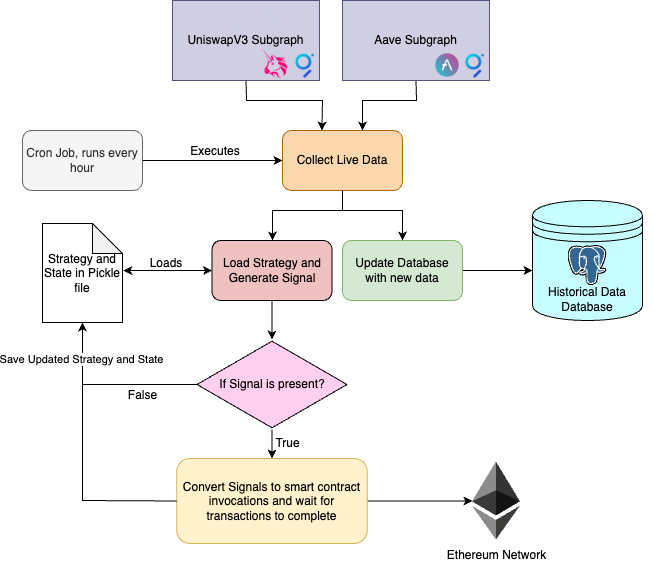
\includegraphics[width=0.99\textwidth]{project/Images/live-trading-system-diagram.png}
    \caption{Flowchart of trading a strategy live \label{fig:live-flow}}
\end{figure}

\subsection{Smart Contracts}
\label{sec:smart-contracts}
In order to be able to interact with Uniswap and Aave over Ethereum, smart contracts are written, which are then deployed on the blockchain network. Functions that the smart contract possesses can then be executed by anyone who knows the contract's address on the network. Smart contracts are programmable protocols written in Solidity, a high-level programming language designed for creating and executing smart contracts on Ethereum. For trading using the mentioned strategies, a few the following functionalities are required to be implemented; wrapping ETH for WETH, unwrapping WETH, swapping token A for token B using a given liquidity pool and finally, borrowing and repaying some of token A using WETH as collateral. The first two functions are required if the trader has only ETH in their account; thus, by wrapping the ETH, they can trade ETH as an ERC-20 token.

\subsubsection{Wrapping of ETH and Unwrapping WETH}
This functionality is required if the trader has only ETH in their account; thus, by wrapping the ETH, they could trade ETH in its ERC-20 format, WETH. ERC-20 is a widely adopted technical standard to create interchangeable Ethereum blockchain tokens. It provides developers with the framework to design tokens compatible with various applications and services operating within the Ethereum ecosystem. These tokens are designed to represent a variety of assets, most importantly cryptocurrencies. The functions of these functionalities can be seen below, where \texttt{swapEthForWeth} wraps ETH and \texttt{swapWethForEth} unwraps WETH. The \texttt{swapEthForWeth} function first uses the \texttt{IWETH} interface, which is itself an ERC20 interface, to allow functions such as transfer of ownership of the token, to deposit an amount of ETH in exchange for WETH, which is then transferred back to the address of the caller. The \texttt{swapWethForEth} function unwraps the WETH by first sending the specified volume of WETH from the caller to the smart contract, withdrawing the specified amount from the IERC20, which calls the \texttt{receive} function to enable the receiving of ETH and once the ETH is withdrawn into the smart contract's account, it is transferred back to the caller.
\begin{lstlisting}[language=Solidity]
interface IWETH is IERC20 {
  function deposit() external payable;
  function withdraw(uint amount) external;
}

address public immutable wethAddress = 0xC02aaA39b223FE8D0A0e5C4F27eAD9083C756Cc2;

function swapEthForWeth() external payable {
    IWETH weth = IWETH(wethAddress);
    weth.deposit{ value: msg.value }();
    weth.transfer(msg.sender, msg.value);
}

function swapWethForEth(uint256 amount) external payable {
    IWETH(wethAddress).transferFrom(msg.sender, address(this), amount);
    IWETH(wethAddress).withdraw(amount);
    msg.sender.transfer(address(this).balance);
}

receive() external payable {}
\end{lstlisting}

\subsubsection{Swapping using a Uniswap Liquidity Pool}
Swapping using a Uniswap liquidity pool is also another critical functionality. This is done by using the \texttt{IUniswapV3Pool} interface to expose the liquidity pool's functions and calling swap on it using the necessary parameters. The parameters, in their respective order, are the address of the recipient of the swapped tokens, a boolean on whether the swap direction is from token0 to token1 or vice versa, the volume of the source token that would like to be swapped, an integer (sqrtPriceLimitX96) that manages how much slippage is acceptable, and finally abi encoded data that is used in the callback function. When calling \texttt{swap} function, the sqrtPriceLimitX96 parameter is set to ignore the effects of slippage and proceed with the swap. Finally, once the swap has taken place, Uniswap calls the callback function \texttt{uniswapV3SwapCallback}, with transfers the swapped tokens to the caller of the function.

\begin{lstlisting}[language=Solidity]
function swapExactUsingPool(address poolAddress, bool zeroForOne, int256 amountIn) public returns (int256, int256) {
    IUniswapV3Pool pool = IUniswapV3Pool(poolAddress);
    return
        pool.swap(msg.sender, zeroForOne, amountIn, zeroForOne ? TickMath.MIN_SQRT_RATIO + 1 : TickMath.MAX_SQRT_RATIO - 1, abi.encode(poolAddress, pool.token0(), pool.token1(), msg.sender));
}

function uniswapV3SwapCallback(int256 amount0Delta, int256 amount1Delta, bytes calldata data) external override {
    (address poolAddress, address token0, address token1, address userAddress) = abi.decode(data, (address, address, address, address));
    require(msg.sender == address(poolAddress));
    if (amount0Delta > 0) {
        IERC20(token0).transferFrom(
            userAddress,
            msg.sender,
            uint256(amount0Delta)
        );
    }
    if (amount1Delta > 0) {
        IERC20(token1).transferFrom(
            userAddress,
            msg.sender,
            uint256(amount1Delta)
        );
    }
}
\end{lstlisting}

\subsubsection{Borrowing and Repaying Tokens using Aave}
To allow for short selling, borrowing and repaying tokens are required; therefore, interacting with Aave in the smart contract is essential. The first step is to instantiate the lending pool using Aave's \texttt{PoolAddressesProvider}. When borrowing, some collateral is set aside to be able to borrow any number of tokens; thus, the first step is to deposit this collateral into the lending pool and allow it to be used as collateral (Lines 1-8). Secondly, the specified token is borrowed from the lending pool using the variable interest rate specified by the third argument in the \texttt{borrow} function; once received, the tokens are sent to the caller's address. The opposite methodology is true for loan repayment; the tokens are transferred from the caller's address to the smart contract's address, which is then sent back to the lending pool by the \texttt{repay} function. The collateral is withdrawn and automatically sent to the caller's address.
\begin{lstlisting}[language=Solidity]
IPool public immutable lendingPool = IPool(IPoolAddressesProvider(0x2f39d218133AFaB8F2B819B1066c7E434Ad94E9e).getPool());

function borrowToken(address tokenAddress, uint256 borrowAmount, uint256 collatoralAmount) public {
    // Deposit Collatoral
    IERC20(wethAddress).transferFrom(msg.sender, address(this), collatoralAmount);
    IERC20(wethAddress).approve(address(lendingPool), collatoralAmount);
    lendingPool.deposit(wethAddress, collatoralAmount, address(this), 0);
    lendingPool.setUserUseReserveAsCollateral(wethAddress, true);

    // Borrow token
    lendingPool.borrow(tokenAddress, borrowAmount, 2, 0, address(this));
    IERC20(tokenAddress).transferFrom(address(this), msg.sender, borrowAmount);
}

function repayBorrowedToken(address tokenAddress, uint256 repayAmount, uint256 collateralWithdrawAmount) public {
    IERC20(tokenAddress).transferFrom(msg.sender, address(this), repayAmount);
    IERC20(tokenAddress).approve(address(lendingPool), repayAmount);
    lendingPool.repay(tokenAddress, repayAmount, 2, address(this));
    lendingPool.withdraw(wethAddress, collateralWithdrawAmount, msg.sender);
}
\end{lstlisting}

\subsubsection{Opening and Closing of Trading Positions}
In addition to these functions, it is known that batching transactions together is more efficient than having to execute them separately, therefore as the strategies being explored for this project require both a buying and selling trade each time, the functions \texttt{openBuySellPositions} and \texttt{closeBuySellPositions} have been implemented such that it follows the method mentioned in Subsection \ref{sec:buying-selling}.

\begin{lstlisting}[language=Solidity]
function openBuySellPositions(address buyPoolAddress, bool buyZeroForOne, int256 buyAmount, address sellTokenAddress, uint256 sellAmount, uint256 collatoralAmount, address sellPoolAddress, bool sellZeroForOne) external {
        swapExactUsingPool(buyPoolAddress, buyZeroForOne, buyAmount);
        borrowToken(sellTokenAddress, sellAmount, collatoralAmount);
        swapExactUsingPool(sellPoolAddress, sellZeroForOne, int256(sellAmount));
}

function closeBuySellPositions(address buyPoolAddress, bool buyZeroForOne, int256 buyAmount, address sellTokenAddress, uint256 sellAmount, uint256 collatoralAmount, address sellPoolAddress, bool sellZeroForOne
    ) external {
        swapExactUsingPool(buyPoolAddress, buyZeroForOne, buyAmount);
        swapExactUsingPool(sellPoolAddress, sellZeroForOne, int256(sellAmount));
        repayBorrowedToken(sellTokenAddress, sellAmount, collatoralAmount);
}
\end{lstlisting}

\subsection{State}
Storing the state of the strategy is essential as the strategies need to store and maintain its history and variables to ensure consistency when trading; therefore, the state is stored as a dictionary in a pickle file. The state contains the liquidity pool pair being traded, the strategy instance, a dictionary of the open positions (initially empty) and the account balance. The state is updated after every execution and stored in the pickle file.

\subsection{Retreival of Data and Signal Generation}
The frequency at which signals and data are collected is easily variable; however, the current design has a frequency of every hour to ensure consistency. This frequency is set in a Cron job. The Cron job runs a script to collect the current price data and generate a signal. Using Uniswap's subgraph, two queries are sent to retrieve the necessary data. The first query queries the liquidity pool returning its current prices, and the second, retrieves the most recent transaction, regardless of the type of transaction, to collect the cost of gas at the time. These data points are inserted into their corresponding tables in the database. They are also sent to the strategy to generate a signal, which is sent to the execution system for execution. The GraphQL queries are in Appendix \ref{app:live-pool-price-query} and \ref{app:live-gas-query}.

\subsection{Trade Execution}
Once the signal has been received, it is sent to the trade execution system. Once the signal is required to be actualized, the execution system breaks the signal into different types of orders and executes them. For each type of order in signal, its parameters are extracted, e.g. volume to buy, volume to sell, the target token and the prices when opening a position. These parameters are then used to calculate the remaining parameters required to call the corresponding smart contract function, e.g. the swap direction's zeroForOne. Finally, once all the necessary function parameters have been defined, the order is executed on the blockchain by performing four steps. The first is calling the smart contract function, signing the transaction, sending the transaction and waiting for the transaction to complete.
\begin{lstlisting}[language=Python]
# Call the order's corresponding function
call_function = contract.functions.<Smart Contract Function Name>(<Function Paramters>).buildTransaction({"chainId": Chain_id, "from": caller, "nonce": nonce})
# Sign transaction
signed_tx = web3.eth.account.sign_transaction(call_function, private_key=private_key)
# Send transaction
send_tx = web3.eth.send_raw_transaction(signed_tx.rawTransaction)
# Wait for transaction receipt
tx_receipt = web3.eth.wait_for_transaction_receipt(send_tx)
\end{lstlisting}

\noindent After all of the orders have been executed, the new balances of each token along with the updated \texttt{open\_positions} is returned to then be stored as the new state.

\chapter{Trading Strategies}
\label{sec:strats}
As previously mentioned, the strategy I employ is the mean reversion trading strategy. The basic concept of a mean reversion strategy identifying two closely related assets or securities, typically referred to as a pair, and taking advantage of deviations from their historical price relationship. This works by initially identifying a pair of assets that have a historically stable relationship as I have done in Section \ref{sec:liquidity-pools}. Then as prices change you calculate the spread, which is the difference between their prices. Look for deviations from the historical mean spread, upon a deviation one buys the undervalued asset and sells the other. The positions are then closed once the spread reverts back to its historical mean.

\section{Abstract Strategy}
The implementation of the generalization of these strategies is intricate and designed to be scalable and highly customizable with various parameters. Additionally, since the trading strategies being investigated are based on mean reversion, an abstract strategy is created to allow for quick exploration and research into different approaches and the impact of hedge ratio calculations on returns. This abstract strategy encompasses the core logic of generating trading signals, determining optimal trade timing and volumes, and transmitting them to the live or backtesting system. The strategy-specific classes contain operations that calculate the hedge ratio and establish the thresholds that trigger the generation of trading signals. Below shows the functions that the abstract strategy possesses.
\vspace{5mm}
\begin{lstlisting}[language=Python]
class Abstract_Strategy():
    def __init__(self, number_of_sds_from_mean, window_size_in_seconds, percent_to_invest, strategy_name, gas_price_threshold, rebalance_threshold_as_percent_of_initial_investment):
        ...

    def initialise_historical_data(self, history_p1, history_p2):
        ...

    def recalculate_thresholds(self, has_trade=False):
        raise NotImplementedError("recalculate_thresholds not implemented")

    def new_tick(self, price_of_pair1, price_of_pair2, has_trade):
        ...

    def generate_signal(self, ctx, prices):
        ...

\end{lstlisting}
\vspace{5mm}

The functions \texttt{\_\_init\_\_,\ initialise\_historical\_data,\ new\_tick} and \texttt{generate\_signal} are all inheritted by each strategy and \texttt{recalculate\_thresholds} is implemented in each instance of the strategy. \texttt{\_\_init\_\_,\ initialise\_historical\_data} are self explanatory. \texttt{new\_tick} is called in \texttt{generate\_signal} to update the strategy's knowledge of historical prices, this function also triggers a call to \texttt{recalculate\_thresholds} which re-calculates the hedge ratio and determines the thresholds at which an arbitrage opportunity becomes apparent. \texttt{generate\_signal} is the function that is called by the trading system at each price update, it first invokes \texttt{new\_tick} which in turn updates the thresholds, finally the updated hedge ratio and thresholds are used in the process of generating a signal. The steps of \texttt{generate\_signal} are outlined below:
\begin{enumerate}
    \item The first step is to call \texttt{new\_tick} which updates the thresholds
    \item Second, is to check whether a position is already held;
    \begin{enumerate}
        \item If a position IS held, the first is to check if the spread is between the thresholds and if the gas price is below that the specified limit, the positions are closed. Otherwise, the loan to value health factor is calculated, if it may cause liquidation, additional collateral is deposited in Aave.
        \item However, if a position is NOT held and the gas price is below that the specified limit, there are 3 cases. \begin{enumerate}
            \item $spread > upper\_threshold$ - Buy pair 2 and sell pair 1
            \item $spread > lower\_threshold$ - Buy pair 1 and sell pair 2
            \item No trade
        \end{enumerate}
        Furthermore, if a trade is ordered, it is also checked, if the WETH balance falls below the rebalance threshold, the additional tokens are converted back to WETH.
    \end{enumerate}
    In addition, prior to opening or closing a position, a preliminary check is conducted to ensure that the ETH balance remains positive. If the anticipated balance after executing the orders indicates a potential shortfall, an order to \texttt{BUY\ ETH} is automatically initiated. This precautionary measure ensures that the strategy maintains a positive ETH balance and avoids entering into positions that could lead to negative balances.
\end{enumerate}

\subsection{Volume of Trades}
A major part of the strategy is at which volumes to trade, therefore in order to be able to trade the maximum amount a minimization problem must be solved. However, before delving into thie problem it is important to highlight the influence of the hedge ratio of the trading volumes. If the hedge ratio is positive, for every unit of pair0 traded, \texttt{hedge\_ratio} units of pair1 should be traded. However, the inverse is true if the hedge ratio is negative, for every \texttt{-hedge\_ratio} units of pair0 traded, 1 unit of pair1 should be traded.
\\[5mm]
Given that $Z$ is amount of WETH in the account, $p_0, p_1$ are the prices of pairs 0 and 1 respectively, $LTV$ is the loan-to-value ratio and $x, y$ are the volumes to be traded on pair0 and pair1 respectively. Additionally, to generalize the problem for both positive and negative hedge ratios, let $n:k$ represent the ratio of volume traded for pair0:pair1. Assuming we are buying pair0 and selling pair1. The following problem states finds the maximum volumes that can be traded to leave the least amount of WETH remaining.
\begin{equation}
\begin{aligned}
\min_{x, y} \quad & Z - xp_0 - \frac{yp_1}{LTV}\\
\textrm{s.t.} \quad & x = \frac{k}{n}y\\
    &x, y \geq 0\\
    &p_0, p_1 \geq 0\\
    &Z \geq 0\\
    &0 \leq LTV \leq 1\\
\end{aligned}
\end{equation}
Therefore, as all terms in the objective function are positive therefore, the minimal objective value in theory must be 0:
\begin{align*}
    Z - xp_0 - \frac{yp_1}{LTV} &= 0\\
    Z - \frac{k}{n}yp_0 - \frac{yp_1}{LTV} &= 0\\
    Z - (\frac{k}{n}p_0 + \frac{p_1}{LTV})y &= 0\\
    y &= \frac{Z}{\frac{k}{n}p_0 + \frac{p_1}{LTV}}\\
    x &= \frac{k}{n}\frac{Z}{\frac{k}{n}p_0 + \frac{p_1}{LTV}}
\end{align*}
\noindent Thus the resulting values of $x$ and $y$ represent the solution that minimizes the problem while maximizing the tradable volume. The case above shows that $x$ units of pair0 can be bought and thus $y$ units of pair1 must be sold. Similarly, if pair0 is sold and pair1 is bought, the maximum volumes are determined by $x = \frac{Z}{\frac{p_0}{LTV} + \frac{n}{k}p_1}$ and $y = \frac{n}{k} \frac{Z}{\frac{p_0}{LTV} + \frac{n}{k}p_1}$.

\section{Constant Hedge Ratio Strategy}
In the most simplistic mean reversion strategy, the approach relies on a given historical dataset, assuming that the hedge ratio between the paired assets remains consistent over the long term. To determine this hedge ratio, the Ordinary Least Squares (OLS) regression method is employed. In Python, the calculation can be carried out using the following steps:
\vspace{5mm}
\begin{lstlisting}[language=Python]
model = sm.OLS(history_p1, sm.add_constant(history_p2))
results = model.fit()
# Gradient of the OLS i.e. X = results.params[0] + results.params[1] * 'p2_token1_price'
hedge_ratio = params[1]
\end{lstlisting}
\vspace{5mm}
In Figure \ref{fig:f1}, the observed trend reveals that the gradient, representing the rate of change, exhibits a proximity to the value of 1. This indicates a relatively balanced relationship between the prices of each pair. However, it is important to note that as time progresses, any fluctuations or deviations from the exact value of 1 are minimal and have a negligible impact on the overall trend. The stability of the gradient over time suggests a consistent and relatively stable relationship between the liquidity pools, reinforcing the notion that their interdependence remains relatively constant.
\begin{figure}[!htb]
    \centering
    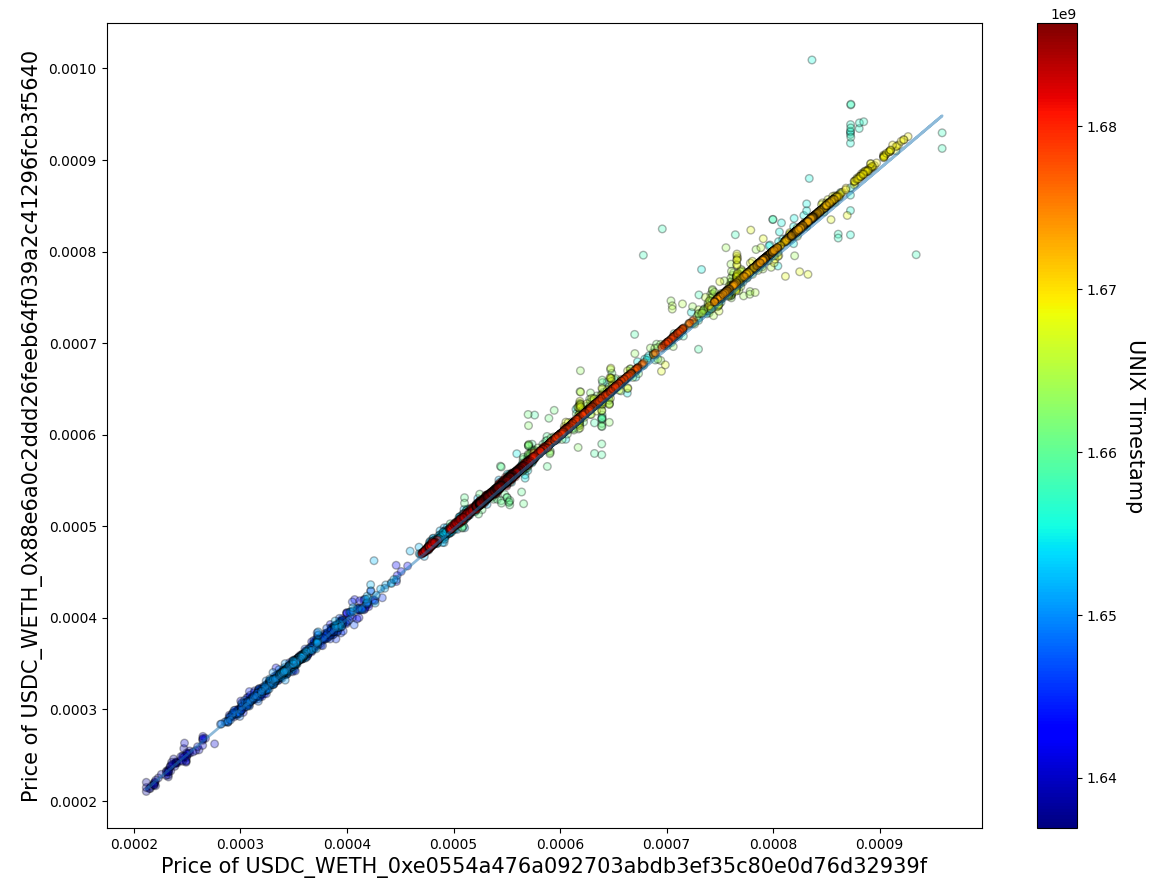
\includegraphics[width=0.8\textwidth]{project/Images/simple_hedge_ratio.png}
    \caption{Conducting OLS to obtain the Hedge Ratio \label{fig:f1}}
\end{figure}

\section{Sliding Window Strategy}
As mentioned earlier, the hedge ratio plays a crucial role in minimizing risk and achieving a market-neutral position in trading strategies. However, employing a static hedge ratio may prove suboptimal since market conditions and the correlation between paired assets can evolve over time. To tackle this challenge, a dynamic approach is adopted using a sliding window approach. In this approach, the hedge ratio is continuously updated at each tick by considering the most recent data. The length of the data window used for the calculation is determined by the value specified in the \texttt{window\_size} argument. By incorporating the sliding window mechanism, the hedge ratio remains adaptive to the changing market dynamics, providing a more accurate and responsive estimation for effective risk management and trading decisions. Therefore, the following function is ran every price tick,
\vspace{5mm}
\begin{lstlisting}[language=Python]
def update_hedge_ratio(self):
    p1, p2 = self.history_p1[-window_size:], self.history_p2[-window_size:]
    model = sm.OLS(p2, sm.add_constant(p1))
    results = model.fit()
    self.hedge_ratio = results.params[1]
\end{lstlisting}

\section{Lagged Strategy}
A lagged strategy was also a implemented as an extension of the sliding window strategy. In the context of the sliding window strategy, the hedge ratio is updated using the most recent data within a specified window size. However, due to potential delays or lags in the synchronization of liquidity pools, the instantaneous prices of the assets may not fully reflect their actual relationship. Therefore, this approach aims to account for potential lags in the synchronization of liquidity pools. The lagged strategy extends the existing sliding window approach by using \texttt{sm.tsa.lagmat} function to perform the lag, which is then used to perform OLS.
\vspace{5mm}
\begin{lstlisting}[language=Python]
def update_hedge_ratio(self):
    maxlag = min(self.lag, min(self.window_size_in_hours, len(self.history_p1))-1)
    p1, p2 = self.history_p1[-(self.window_size_in_hours+maxlag):], self.history_p2[-self.window_size_in_hours:]
    lagged_p1 = sm.tsa.lagmat(p1, maxlag=maxlag)[-self.window_size_in_hours:]
    model = sm.OLS(p2, sm.add_constant(lagged_p1))
    results = model.fit()
    self.hedge_ratio = results.params[1]
\end{lstlisting}

\section{Granger Causality Test}
Similarly, to account for lag and causality, a strategy that was employed was using the Granger Causality Test. The Granger Causality Test is a statistical hypothesis test that assesses the predictive value of one time series in forecasting another. Part of the test the results provide insights into the relationship between the variables and help determine the presence of Granger causality in the form of an OLS regression for both the restricted and unrestricted models. The restricted model is a regression model that includes only the lagged values of the dependent variable whereas the unrestricted model includes both the lagged values of the dependent variable and the potentially causal variable. The restricted model's regression parameters are used to calculate the hedge ratio.
\vspace{5mm}
\begin{lstlisting}[language=Python]
def update_hedge_ratio(self):
    p1, p2 = self.history_p1, self.history_p2
    data = pd.DataFrame({'Asset1': p1, 'Asset2': p2})
    granger_results = statsmodels.tsa.stattools.grangercausalitytests(data, maxlag=[1], verbose=False)
    self.hedge_ratio = granger_results[1][1][0].params[0]
\end{lstlisting}

\section{Kalman Filter Strategy}
Another method that is often used to ensure market-neutral positions is the use of Kalman Filters as a dynamic tool to update and adapt the hedge ratio, taking into account the changing market conditions and the evolving relationship between the paired assets. This allows for a more responsive and adaptive approach to maintaining a market-neutral position. The Kalman Filter takes into consideration not only the current price data but also the historical information and the underlying dynamics of the assets. It provides a more robust and accurate estimation of the optimal hedge ratio, which aligns with the mean reversion strategy's objective of capturing potential price divergences and profiting from their eventual convergence.
\\[5mm]
The Kalman Filter works by iteratively updating and refining its estimate of the system state using a prediction step and an update step. For this an initial `guess' of the parameters that I use is the using the Ordinary Least Squares from the historical information provided. The remainder of the parameters that are selected can be seen below:
\vspace{5mm}
\begin{lstlisting}[language=Python]
model = sm.OLS(price_history_2, sm.add_constant(price_history_1))
initial_state = model.fit().params[::-1]

kf = KalmanFilter(
    n_dim_state=2,
    initial_state_mean=initial_state,
    transition_matrices=np.eye(2),
    observation_matrices=obs_mat,
    transition_covariance=1e-5 * np.eye(2)
    )
\end{lstlisting}
\vspace{5mm}

\noindent Below describes the reasoning behind the choices of parameters:
\begin{itemize}
    \item \texttt{n\_dim\_state} - This parameter to the number of elements in the state. In our scenario, the state consists of two components: the y-intercept and the gradient.
    \item \texttt{initial\_state\_mean} - As mentioned earlier, the Kalman Filter utilizes past estimates to iteratively estimate the true states. Therefore, I employ the OLS method to calculate the initial state of the price history's regression, which returns both the y-intercept and gradient.
    \item \texttt{observation\_matrices} - The observation matrix defines the relationship between the observed measurements and the hidden state variables. Thus takes the historical data that is provided zipped along with 1 as the observed measurements directly correspond to the hedge ratio. This can be represented as $\begin{bmatrix} y_1 & 1 \\ y_1 & 1 \\ \vdots & 1 \\ y_n & 1\end{bmatrix}$.
    \item \texttt{transition\_matrices} - In the context of our strategy, we anticipate a consistent long-term hedge ratio. Therefore, we set the \texttt{transition\_matrices} parameter to $\begin{bmatrix} 1 & 0\\ 0 & 1 \end{bmatrix}$.
    \item \texttt{transition\_covariance} - Finally the transition\_covariance specifies the covariance matrix of the process noise. It represents the uncertainty or variability in the state transition, hence it is set to be very small, $\begin{bmatrix} 10^{-5} & 0\\ 0 & 10^{-5} \end{bmatrix}$.
\end{itemize}

Figures \ref{fig:evolving_hedge_ratio_kf} and \ref{fig:ratios_kf} provide visual representations of the hedge ratio's evolution over time. These figures illustrate that the hedge ratio, while exhibiting subtle variations, does indeed change over the observed period. One notable event is the significant drop that occurs at the timestamp 1.655e9 or June 2022. This particular shift in the hedge ratio is likely attributed to the migration from the Proof of Work (PoW) consensus mechanism to the Proof of Stake (PoS) consensus mechanism on the Ethereum network.
\\[5mm]
During the transition from PoW to PoS, there are fundamental changes in how the Ethereum network reaches consensus and validates transactions. This change in consensus mechanism can impact various aspects of the network, including the dynamics of the hedge ratio. It is plausible that the observed drop in the hedge ratio during the migration period reflects the adjustments and reconfiguration of the underlying mechanisms in response to the shift to PoS.

\begin{figure}[!htb]
    \centering
    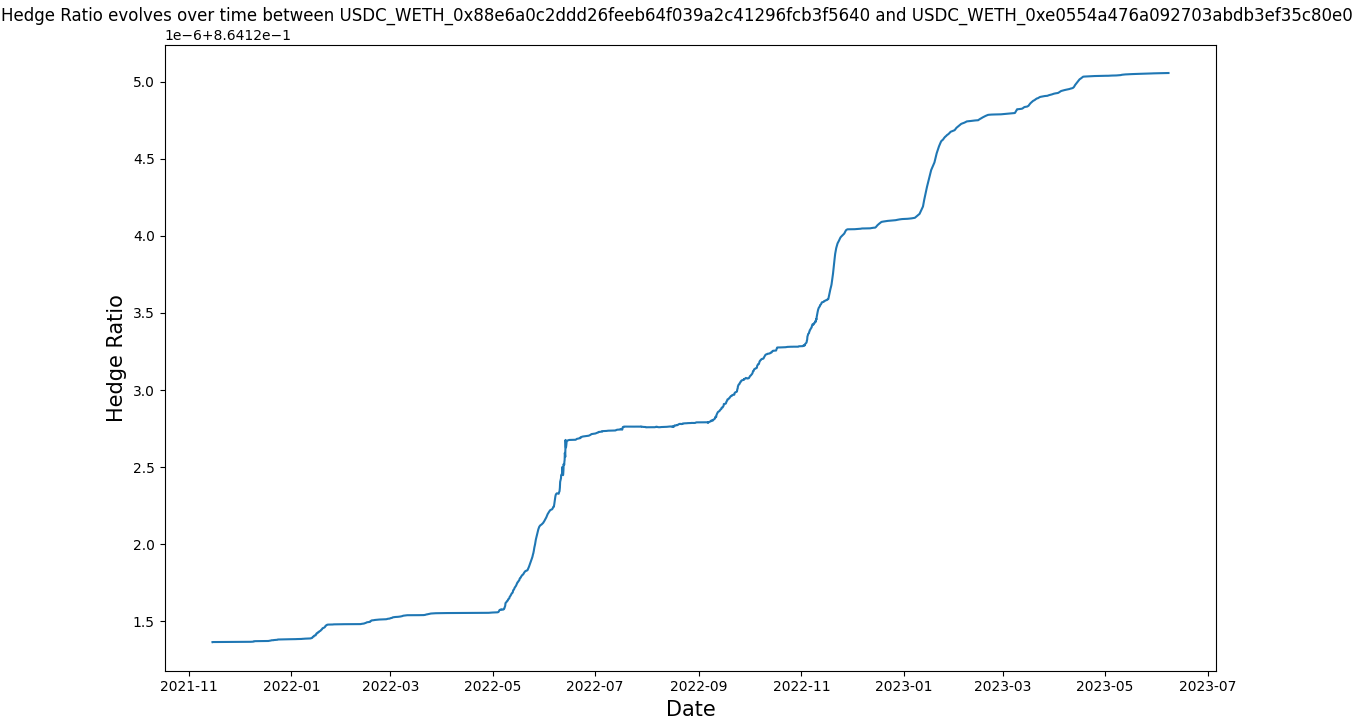
\includegraphics[width=\textwidth]{project/Images/Evolving_hedge_ratio_kf.png}
    \caption{Plot of how the Hedge Ratio using the Kalman Filter \label{fig:evolving_hedge_ratio_kf}}
\end{figure}

\begin{figure}[!htb]
    \centering
    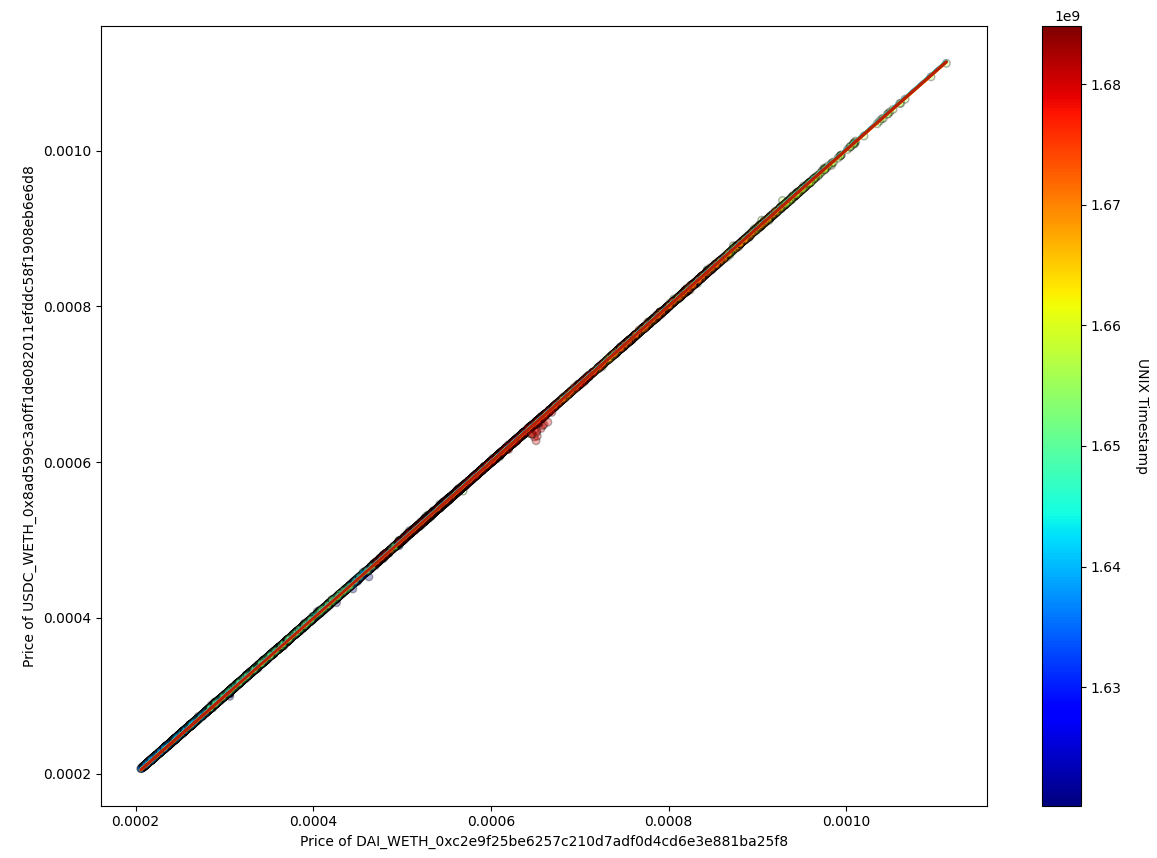
\includegraphics[width=\textwidth]{project/Images/plots_1.png}
    \caption{The plot shows the Kalman Filter estimating the regression line over time, \label{fig:ratios_kf}}
\end{figure}


\chapter{Evaluation}
\definecolor{green}{RGB}{0,153,0}
The design of each strategy and the backtesting system allows for extensive parameterisation, providing multiple axes for analysis. Parameters that can be adjusted are at what number of standard deviations away from the mean spread a threshold should be set and a signal to be generated, how the trades are executed, limits on how much gas price should be when executing a trade, and also the volume of the initial investment. These are all factors that can affect the returns of the trading strategy. In the following sections, we will examine the strategy's performance by varying these parameters, providing valuable insights into their influence on trading outcomes. For data visualisation, we denote the liquidity pool pairs by their index; see Table \ref{tab:pool-labels}. Note that \textcolor{red}{-100\%} in the tables below indicate one of the token's balance in the account falls below 0, resulting in bankruptcy.
\begin{table}[!ht]
    \centering
    \begin{adjustwidth}{-0.5in}{-0.9in}
        \begin{tabular}{|p{20em}|p{20em}|p{3em}|}\hline
            Pool1 & Pool2 & Label\\\hline
            \truncate{20em}{USDC\_WETH\_0x88e6a0c2ddd26feeb64f039a2c41296fcb3f5640} & \truncate{20em}{USDC\_WETH\_0xe0554a476a092703abdb3ef35c80e0d76d32939f} & 0\\\hline
            \truncate{20em}{USDC\_WETH\_0x8ad599c3a0ff1de082011efddc58f1908eb6e6d8} & \truncate{20em}{USDC\_WETH\_0xe0554a476a092703abdb3ef35c80e0d76d32939f} & 1\\\hline
            \truncate{20em}{WETH\_USDT\_0x11b815efb8f581194ae79006d24e0d814b7697f6} & \truncate{20em}{USDC\_WETH\_0xe0554a476a092703abdb3ef35c80e0d76d32939f} & 2\\\hline
            \truncate{20em}{WETH\_USDT\_0x4e68ccd3e89f51c3074ca5072bbac773960dfa36} & \truncate{20em}{USDC\_WETH\_0xe0554a476a092703abdb3ef35c80e0d76d32939f} & 3\\\hline
            \truncate{20em}{DAI\_WETH\_0x60594a405d53811d3bc4766596efd80fd545a270} & \truncate{20em}{USDC\_WETH\_0xe0554a476a092703abdb3ef35c80e0d76d32939f} & 4\\\hline
            \truncate{20em}{DAI\_WETH\_0xc2e9f25be6257c210d7adf0d4cd6e3e881ba25f8} & \truncate{20em}{USDC\_WETH\_0xe0554a476a092703abdb3ef35c80e0d76d32939f} & 5\\\hline
            \truncate{20em}{USDC\_WETH\_0xe0554a476a092703abdb3ef35c80e0d76d32939f} & \truncate{20em}{WETH\_USDT\_0xc5af84701f98fa483ece78af83f11b6c38aca71d} & 6\\\hline
        \end{tabular}
    \end{adjustwidth}
    \caption{Liquidity pool pairs and their corresponding labels \label{tab:pool-labels}}
\end{table}
\vspace{-4ex}
\section{Trading System}
The implemented backtesting system is designed to be robust and comprehensive, considering all the necessary costs associated with trading, as discussed in Section \ref{sec:backtesting-sys}. However, factors such as data granularity and accounting for slippage are some areas that could benefit from further improvement.
\\[3mm]
One aspect that could be enhanced is the data granularity of the pricing data used in the backtesting system. Currently, the system uses hourly data points, which may not capture all the price movements and volatility. By incorporating more granular data, such as minute-by-minute or even tick-level data, the system could provide a more accurate representation of market dynamics and potentially improve the accuracy of the backtest results.
\\[3mm]
Additionally, when executing swaps or trades, it is important to consider the impact of slippage. Slippage refers to the price difference that occurs when executing a trade due to changes in the market conditions, such as supply differences between trading pairs. To account for slippage, the system should incorporate realistic price adjustments to accurately simulate the trading environment. This can help ensure that the backtest results reflect the actual performance in real trading scenarios. However, this is somewhat mitigated as only larger liquidity pools, with a volume of $\geq \$10 million$, are used and with only a maximum of 100ETH (\$394,626.00) being traded in each pool, the effects of slippage become very small in such scenarios.
\\[3mm]
By addressing these aspects, refining the data granularity, and furthering the slippage considerations, the backtesting system can provide more precise and reliable results, leading to improved insights into the profitability and viability of the trading strategy under evaluation.

\section{Strategy Parameters}
\label{sec:strat-param}

\subsection{Number of Standard Deviations away from the mean}
Varying the standard deviation in a mean reversion pairs trading strategy can significantly impact the strategy's returns. When the number of standard deviations is too high, the spread between the pair's prices must deviate significantly from the mean before generating a signal. In this case, the strategy may generate fewer trades, resulting in longer holding periods for positions; however, this tends to have a greater return per trade. On the other hand, setting a lower number of standard deviations makes the strategy more sensitive to smaller deviations from the mean. This increases the frequency of trade signals and potentially leads to more active trading. However, it also exposes the strategy to a higher risk of false signals or trading on noise in the price data. It can result in higher transaction costs and potentially lower returns due to increased trading activity, potentially resulting in losses. For simplicity, $\#_{\sigma}$ denotes this parameter.
\\[3mm]
Table \ref{tab:varying_sigma} displays the returns as the standard deviations away from the mean the threshold is set. For this experiment, the other parameters were; 100 ETH worth of initial investment, the window size set to 30 days, a gas price threshold of 1 ETH (i.e. not having a threshold), the interactions with the blockchain to be separately executed and finally the lag that the lagged strategy uses are set to 1 hour. The period that trading occurs is from 18th December 2021 to 9th June 2023.
\\[3mm]
We can see that as $\#_{\sigma} \rightarrow 0$, the number of trades increases; however, this causes the returns to be more negative (and in some cases terminating early with 100\% loss) than positive, likely due to trades being opened when gas fees are substantially larger than the profit. However, if $\#_{\sigma}$ is larger, although the profits from each trade increase, the number of actionable opportunities is limited. Another interesting feature that can easily be spotted is that the Constant Hedge Ratio Strategy makes little to no profit in all cases. In contrast, the other strategies perform better as $\#_{\sigma} \rightarrow \sim 1.75$. Furthermore, all strategies return a loss on pool pair 6 except the Kalman Filter Strategy, albeit with a higher threshold.
\\[3mm]
Consistent profit among all pool pairs, excluding pool pair 6, is also achieved at different numbers of standard deviations. We can see in Figure \ref{fig:varyStd} that the average return across all liquidity pool pairs that each strategy generates at each standard deviation. The Kalman Filter becomes largely profitable at $\#_{\sigma} = 0.5$, whereas the lagged and sliding window strategies become profitable at $\#_{\sigma} = 2$. This is because the Kalman Filter and the Granger Causality tests can better find underlying trends, thus better selecting the hedge ratio, affecting the volumes being traded and hence the effect of the returns.

\begin{table}[!htb]
    \centering
    \begin{adjustwidth}{-0.8in}{-0.9in}
        \begin{tabular}{|p{4em}|p{2em}|p{3em}|p{3em}|p{3em}|p{3em}|p{3em}|p{3em}|p{3em}|p{3em}|p{3em}|p{3em}|}\hline
            Std & Pool Pair & \multicolumn{10}{|c|}{Strategy's Annual Percentage Rate (APR) - Trading from 18th December 2021 to 9th June 2023} \\\cline{3-12}
            &   & \multicolumn{2}{|c|}{Constant} & \multicolumn{2}{|c|}{Sliding Window} & \multicolumn{2}{|c|}{Lagged} & \multicolumn{2}{|c|}{Granger Causality} & \multicolumn{2}{|c|}{Kalman Filter}\\\cline{3-12}
            & & Return \% & \# of Trades & Return \% & \# of Trades & Return \% & \# of Trades & Return \% & \# of Trades & Return \% & \# of Trades\\\hline

            & 0 & \textcolor{green}{3.66} & 360 & \textcolor{green}{19.02} & 661 & \textcolor{green}{41.18} & 687 & \textcolor{green}{17.8} & 275 & \textcolor{green}{50.66} & 228\\\cline{3-12}
            & 1 & \textcolor{red}{-41.23} & 397 & \textcolor{red}{-70.78} & 660 & \textcolor{red}{-63.39} & 653 & \textcolor{red}{-40.2} & 388 & \textcolor{red}{-10.43} & 307\\\cline{3-12}
            & 2 & \textcolor{green}{3.92} & 454 & \textcolor{red}{-1.43} & 634 & \textcolor{green}{27.81} & 619 & \textcolor{green}{24.64} & 300 & \textcolor{green}{54.06} & 236\\\cline{3-12}
            $\#_{\sigma}=0.1$ & 3 & \textcolor{red}{-53.35} & 535 & \textcolor{red}{-56.31} & 572 & \textcolor{red}{-59.1} & 604 & \textcolor{red}{-33.24} & 375 & \textcolor{red}{-9.76} & 301\\\cline{3-12}
            & 4 & \textcolor{green}{7.42} & 375 & \textcolor{green}{6.72} & 759 & \textcolor{green}{36.73} & 669 & \textcolor{green}{16.18} & 296 & \textcolor{green}{44.35} & 227\\\cline{3-12}
            & 5 & \textcolor{red}{-40.45} & 396 & \textcolor{red}{-61.12} & 587 & \textcolor{red}{-54.1} & 593 & \textcolor{red}{-37.0} & 337 & \textcolor{red}{-17.72} & 328\\\cline{3-12}
            & 6 & \textcolor{red}{-11.0} & 72 & \textcolor{red}{-68.8} & 213 & \textcolor{red}{-62.28} & 198 & \textcolor{red}{-13.58} & 68 & \textcolor{red}{-4.2} & 84\\\hline\hline

            & 0 & \textcolor{green}{7.84} & 723 & \textcolor{red}{-11.01} & 1223 & \textcolor{green}{62.43} & 1185 & \textcolor{green}{66.93} & 550 & \textcolor{green}{130.2} & 378\\\cline{3-12}
            & 1 & \textcolor{red}{-100.0} & 832 & \textcolor{red}{-100.0} & 920 & \textcolor{red}{-100.0} & 936 & \textcolor{red}{-56.1} & 650 & \textcolor{green}{39.26} & 456\\\cline{3-12}
            & 2 & \textcolor{green}{6.14} & 688 & \textcolor{red}{-0.59} & 1105 & \textcolor{green}{73.22} & 1025 & \textcolor{green}{71.64} & 630 & \textcolor{green}{153.85} & 396\\\cline{3-12}
            $\#_{\sigma}=0.5$ & 3 & \textcolor{red}{-84.34} & 794 & \textcolor{red}{-100.0} & 944 & \textcolor{red}{-82.5} & 1063 & \textcolor{red}{-51.1} & 691 & \textcolor{green}{24.18} & 425\\\cline{3-12}
            & 4 & \textcolor{green}{16.97} & 826 & \textcolor{red}{-11.24} & 1243 & \textcolor{green}{66.69} & 1213 & \textcolor{green}{47.5} & 538 & \textcolor{green}{131.36} & 391\\\cline{3-12}
            & 5 & \textcolor{red}{-86.92} & 837 & \textcolor{red}{-100.0} & 854 & \textcolor{red}{-100.0} & 905 & \textcolor{red}{-24.3} & 503 & \textcolor{green}{54.86} & 388\\\cline{3-12}
            & 6 & \textcolor{red}{-27.3} & 124 & \textcolor{red}{-90.13} & 359 & \textcolor{red}{-71.37} & 301 & \textcolor{red}{-3.33} & 56 & \textcolor{red}{-29.04} & 150\\\hline\hline
            
            & 0 & \textcolor{red}{-15.08} & 675 & \textcolor{red}{-1.08} & 864 & \textcolor{green}{75.76} & 865 & \textcolor{green}{60.3} & 586 & \textcolor{green}{93.32} & 442\\\cline{3-12}
            & 1 & \textcolor{red}{-100.0} & 791 & \textcolor{red}{-100.0} & 814 & \textcolor{red}{-85.22} & 1022 & \textcolor{red}{-40.6} & 641 & \textcolor{red}{-7.2} & 505\\\cline{3-12}
            & 2 & \textcolor{red}{-14.94} & 535 & \textcolor{green}{4.72} & 777 & \textcolor{green}{86.24} & 721 & \textcolor{green}{75.65} & 497 & \textcolor{green}{103.11} & 404\\\cline{3-12}
            $\#_{\sigma}=1$ & 3 & \textcolor{red}{-100.0} & 497 & \textcolor{red}{-100.0} & 657 & \textcolor{red}{-64.55} & 872 & \textcolor{red}{-26.11} & 550 & \textcolor{green}{1.42} & 436\\\cline{3-12}
            & 4 & \textcolor{red}{-3.6} & 689 & \textcolor{green}{10.29} & 799 & \textcolor{green}{89.18} & 822 & \textcolor{green}{74.11} & 558 & \textcolor{green}{105.91} & 460\\\cline{3-12}
            & 5 & \textcolor{red}{-100.0} & 533 & \textcolor{red}{-100.0} & 612 & \textcolor{red}{-58.88} & 785 & \textcolor{red}{-25.29} & 500 & \textcolor{green}{26.89} & 408\\\cline{3-12}
            & 6 & \textcolor{red}{-40.18} & 108 & \textcolor{red}{-52.01} & 169 & \textcolor{red}{-34.85} & 125 & \textcolor{red}{-21.08} & 70 & \textcolor{red}{-30.59} & 158\\\hline\hline
            
            & 0 & \textcolor{green}{3.83} & 365 & \textcolor{green}{30.85} & 447 & \textcolor{green}{83.24} & 476 & \textcolor{green}{79.52} & 272 & \textcolor{green}{100.22} & 179\\\cline{3-12}
            & 1 & \textcolor{red}{-100.0} & 408 & \textcolor{red}{-53.49} & 509 & \textcolor{red}{-23.97} & 504 & \textcolor{green}{7.18} & 293 & \textcolor{green}{48.04} & 221\\\cline{3-12}
            & 2 & \textcolor{red}{-4.17} & 302 & \textcolor{green}{14.67} & 402 & \textcolor{green}{68.45} & 391 & \textcolor{green}{79.98} & 250 & \textcolor{green}{96.97} & 147\\\cline{3-12}
            $\#_{\sigma}=1.5$ & 3 & \textcolor{red}{-57.3} & 389 & \textcolor{red}{-44.96} & 453 & \textcolor{red}{-19.47} & 449 & \textcolor{green}{5.83} & 290 & \textcolor{green}{48.86} & 166\\\cline{3-12}
            & 4 & \textcolor{red}{-8.38} & 324 & \textcolor{green}{24.77} & 428 & \textcolor{green}{75.32} & 426 & \textcolor{green}{85.94} & 273 & \textcolor{green}{99.13} & 201\\\cline{3-12}
            & 5 & \textcolor{red}{-100.0} & 312 & \textcolor{red}{-42.04} & 402 & \textcolor{red}{-2.13} & 379 & \textcolor{green}{23.05} & 259 & \textcolor{green}{60.87} & 175\\\cline{3-12}
            & 6 & \textcolor{red}{-31.39} & 77 & \textcolor{red}{-29.45} & 87 & \textcolor{red}{-29.0} & 89 & \textcolor{red}{-13.84} & 35 & \textcolor{red}{-12.98} & 102\\\hline\hline
            
            & 0 & \textcolor{red}{-7.14} & 288 & \textcolor{green}{24.57} & 342 & \textcolor{green}{81.97} & 353 & \textcolor{green}{61.58} & 192 & \textcolor{green}{98.76} & 153\\\cline{3-12}
            & 1 & \textcolor{red}{-52.98} & 358 & \textcolor{red}{-20.9} & 293 & \textcolor{red}{-5.29} & 323 & \textcolor{green}{12.99} & 213 & \textcolor{green}{45.66} & 178\\\cline{3-12}
            & 2 & \textcolor{red}{-1.71} & 225 & \textcolor{green}{21.43} & 277 & \textcolor{green}{68.39} & 270 & \textcolor{green}{68.62} & 180 & \textcolor{green}{95.11} & 133\\\cline{3-12}
            $\#_{\sigma}=1.75$ & 3 & \textcolor{red}{-45.93} & 309 & \textcolor{red}{-14.98} & 268 & \textcolor{red}{-1.01} & 294 & \textcolor{green}{22.19} & 211 & \textcolor{green}{53.56} & 145\\[-3ex]\cline{3-12}
            & 4 & \textcolor{red}{-2.54} & 241 & \textcolor{green}{26.46} & 294 & \textcolor{green}{55.77} & 291 & \textcolor{green}{65.92} & 201 & \textcolor{green}{84.62} & 152\\\cline{3-12}
            & 5 & \textcolor{red}{-41.71} & 287 & \textcolor{red}{-9.73} & 225 & \textcolor{green}{9.79} & 250 & \textcolor{green}{20.48} & 200 & \textcolor{green}{61.97} & 152\\\cline{3-12}
            & 6 & \textcolor{red}{-35.28} & 76 & \textcolor{red}{-19.16} & 67 & \textcolor{red}{-29.96} & 76 & \textcolor{red}{-23.36} & 37 & \textcolor{red}{-16.02} & 74\\\hline\hline
            
            & 0 & \textcolor{green}{1.43} & 226 & \textcolor{green}{28.09} & 271 & \textcolor{green}{54.88} & 268 & \textcolor{green}{35.91} & 141 & \textcolor{green}{64.38} & 116\\\cline{3-12}
            & 1 & \textcolor{red}{-30.57} & 245 & \textcolor{green}{5.14} & 165 & \textcolor{green}{19.55} & 184 & \textcolor{green}{4.65} & 144 & \textcolor{green}{35.95} & 125\\\cline{3-12}
            & 2 & \textcolor{red}{-5.94} & 191 & \textcolor{green}{28.81} & 190 & \textcolor{green}{54.98} & 202 & \textcolor{green}{49.3} & 144 & \textcolor{green}{58.95} & 106\\\cline{3-12}
            $\#_{\sigma}=2$ & 3 & \textcolor{red}{-36.5} & 228 & \textcolor{green}{3.9} & 160 & \textcolor{green}{16.28} & 178 & \textcolor{green}{21.79} & 154 & \textcolor{green}{36.32} & 121\\\cline{3-12}
            & 4 & \textcolor{green}{5.85} & 206 & \textcolor{green}{29.2} & 190 & \textcolor{green}{51.79} & 201 & \textcolor{green}{46.95} & 149 & \textcolor{green}{58.28} & 125\\\cline{3-12}
            & 5 & \textcolor{red}{-19.82} & 192 & \textcolor{green}{7.19} & 138 & \textcolor{green}{21.28} & 147 & \textcolor{green}{12.38} & 138 & \textcolor{green}{42.87} & 125\\\cline{3-12}
            & 6 & \textcolor{red}{-27.18} & 65 & \textcolor{red}{-15.52} & 49 & \textcolor{red}{-17.7} & 54 & \textcolor{red}{-24.53} & 31 & \textcolor{green}{0.67} & 53\\\hline\hline

            
            & 0 & \textcolor{green}{1.75} & 54 & \textcolor{green}{18.68} & 102 & \textcolor{green}{17.31} & 83 & \textcolor{green}{27.63} & 51 & \textcolor{green}{17.88} & 51\\\cline{3-12}
            & 1 & \textcolor{red}{-3.91} & 64 & \textcolor{green}{13.87} & 49 & \textcolor{green}{12.0} & 46 & \textcolor{green}{20.85} & 60 & \textcolor{green}{15.28} & 60\\\cline{3-12}
            & 2 & \textcolor{green}{1.32} & 61 & \textcolor{green}{13.41} & 56 & \textcolor{green}{14.79} & 64 & \textcolor{green}{23.26} & 52 & \textcolor{green}{14.02} & 52\\\cline{3-12}
            $\#_{\sigma}=3$ & 3 & \textcolor{red}{-7.05} & 73 & \textcolor{green}{8.19} & 46 & \textcolor{green}{7.33} & 48 & \textcolor{green}{17.52} & 55 & \textcolor{green}{8.29} & 58\\\cline{3-12}
            & 4 & \textcolor{green}{3.13} & 67 & \textcolor{green}{20.95} & 57 & \textcolor{green}{18.84} & 64 & \textcolor{green}{26.98} & 60 & \textcolor{green}{17.25} & 57\\\cline{3-12}
            & 5 & \textcolor{red}{-4.45} & 53 & \textcolor{green}{13.73} & 39 & \textcolor{green}{12.17} & 39 & \textcolor{green}{23.27} & 51 & \textcolor{green}{17.39} & 57\\\cline{3-12}
            & 6 & \textcolor{red}{-1.17} & 13 & \textcolor{red}{-3.24} & 20 & \textcolor{red}{-2.18} & 25 & \textcolor{green}{3.19} & 5 & \textcolor{green}{8.01} & 16\\\hline
        \end{tabular}
    \end{adjustwidth}
    \caption{Returns of various standard deviation thresholds of each strategy \label{tab:varying_sigma}}.
\end{table}

\begin{figure}[h!]
    \centering
    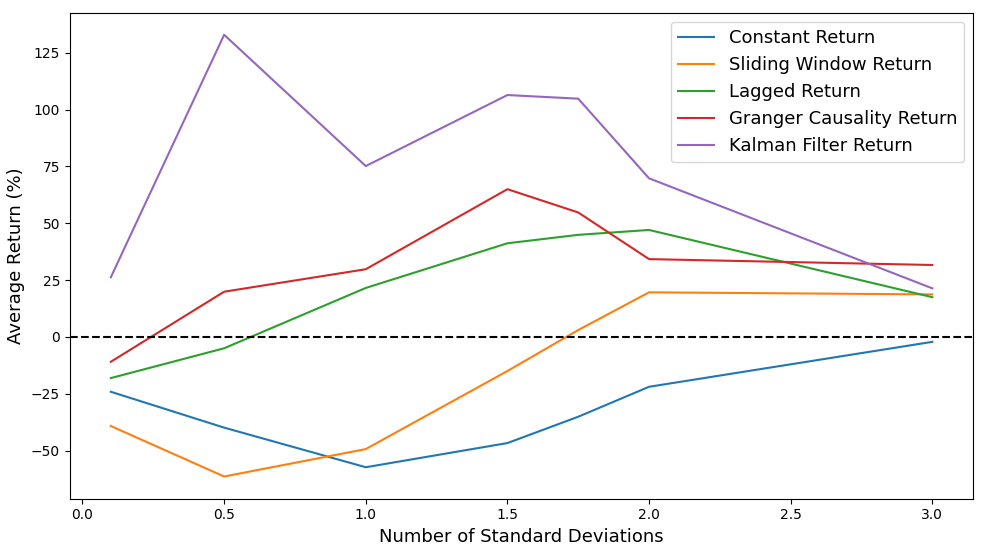
\includegraphics[width=1\textwidth]{evaluation/Images/VaryStd.png}
    \caption{Average Return across all pool pairs using various standard deviations}
    \label{fig:varyStd}
\end{figure}

\subsection{Gas Fees}
Another aspect that could be changed is fees; the first is how the transactions are executed on the blockchain and the maximum gas price if we want to open a position. As previously mentioned, the gas fee is calculated by combining the gas price and the gas used. Therefore, these two parameters allow the strategy to control the gas used and the gas price.

\subsubsection{Batched Transactions vs Separately Executed Transactions}
The method in which the transactions are executed affects how much gas is used. When transactions are executed separately, each transaction incurs its own gas cost. This means that gas will be consumed for various operations such as contract interaction, data storage, and computational tasks for every individual transaction. As a result, executing many separate transactions can lead to a high cumulative gas cost. On the other hand, when transactions are batched together, they are consolidated into a single transaction. This consolidation reduces the overhead associated with executing multiple transactions individually. By combining the operations of multiple transactions into a single execution, redundant computations and storage operations can be eliminated, resulting in more efficient gas usage. It can immediately be seen in Figure \ref{fig:gasResult} that the process of batching the transactions consumes less gas than the combined gas of the transactions required to execute the opening and closing of the positions.
\\[3mm]
Furthermore, the effects of separate versus batched transactions can be seen in Table \ref{tab:BatchedVsSeperate}. The parameters used for this investigation were the same as above with the selection, e.g. $\#_{\sigma} = 1.75$, 100 ETH worth of initial investment, the window size set to 30 days, a gas price threshold of 1 ETH (i.e. not having a threshold) and the testing period remained from 18th December 2021 to 9th June 2023.

\begin{table}[H]
    \centering
    \begin{adjustwidth}{-0.8in}{-0.9in}
        \begin{tabular}{|p{2em}|p{2em}|p{3em}|p{3em}|p{3em}|p{3em}|p{3em}|p{3em}|p{3em}|p{3em}|p{3em}|p{3em}|}\hline
            & Pool Pair & \multicolumn{10}{|c|}{Strategy's Annual Percentage Rate (APR) - Trading from 18th December 2021 to 9th June 2023} \\\cline{3-12}
            &   & \multicolumn{2}{|c|}{Constant} & \multicolumn{2}{|c|}{Sliding Window} & \multicolumn{2}{|c|}{Lagged} & \multicolumn{2}{|c|}{Granger Causality} & \multicolumn{2}{|c|}{Kalman Filter}\\\cline{3-12}
            & & Return \% & \# of Trades & Return \% & \# of Trades & Return \% & \# of Trades & Return \% & \# of Trades & Return \% & \# of Trades\\\hline
            
            \parbox[t]{4em}{\multirow{7}{*}{\rotatebox[origin=c]{90}{Seperate}}} & 0 & \textcolor{red}{-7.14} & 288 & \textcolor{green}{24.57} & 342 & \textcolor{green}{81.97} & 353 & \textcolor{green}{61.58} & 192 & \textcolor{green}{98.76} & 153\\\cline{3-12}
            & 1 & \textcolor{red}{-52.98} & 358 & \textcolor{red}{-20.9} & 293 & \textcolor{red}{-5.29} & 323 & \textcolor{green}{12.99} & 213 & \textcolor{green}{45.66} & 178\\\cline{3-12}
            & 2 & \textcolor{red}{-1.71} & 225 & \textcolor{green}{21.43} & 277 & \textcolor{green}{68.39} & 270 & \textcolor{green}{68.62} & 180 & \textcolor{green}{95.11} & 133\\\cline{3-12}
            & 3 & \textcolor{red}{-45.93} & 309 & \textcolor{red}{-14.98} & 268 & \textcolor{red}{-1.01} & 294 & \textcolor{green}{22.19} & 211 & \textcolor{green}{53.56} & 145\\\cline{3-12}
            & 4 & \textcolor{red}{-2.54} & 241 & \textcolor{green}{26.46} & 294 & \textcolor{green}{55.77} & 291 & \textcolor{green}{65.92} & 201 & \textcolor{green}{84.62} & 152\\\cline{3-12}
            & 5 & \textcolor{red}{-41.71} & 287 & \textcolor{red}{-9.73} & 225 & \textcolor{green}{9.79} & 250 & \textcolor{green}{20.48} & 200 & \textcolor{green}{61.97} & 152\\\cline{3-12}
            & 6 & \textcolor{red}{-35.28} & 76 & \textcolor{red}{-19.16} & 67 & \textcolor{red}{-29.96} & 76 & \textcolor{red}{-23.36} & 37 & \textcolor{red}{-16.02} & 74\\\hline\hline

            \parbox[t]{4em}{\multirow{7}{*}{\rotatebox[origin=c]{90}{Batched}}} & 0 & \textcolor{red}{-2.2} & 288 & \textcolor{green}{30.8} & 342 & \textcolor{green}{87.79} & 353 & \textcolor{green}{66.76} & 192 & \textcolor{green}{100.13} & 153\\\cline{3-12}
            & 1 & \textcolor{red}{-47.23} & 358 & \textcolor{red}{-16.28} & 293 & \textcolor{green}{0.91} & 323 & \textcolor{green}{16.58} & 213 & \textcolor{green}{46.78} & 178\\\cline{3-12}
            & 2 & \textcolor{green}{2.63} & 225 & \textcolor{green}{28.29} & 277 & \textcolor{green}{74.07} & 270 & \textcolor{green}{75.52} & 180 & \textcolor{green}{97.43} & 133\\\cline{3-12}
            & 3 & \textcolor{red}{-42.06} & 309 & \textcolor{red}{-9.95} & 268 & \textcolor{green}{4.71} & 294 & \textcolor{green}{25.33} & 211 & \textcolor{green}{52.93} & 145\\\cline{3-12}
            & 4 & \textcolor{green}{1.72} & 241 & \textcolor{green}{29.97} & 294 & \textcolor{green}{62.84} & 291 & \textcolor{green}{69.21} & 201 & \textcolor{green}{86.18} & 152\\\cline{3-12}
            & 5 & \textcolor{red}{-37.04} & 287 & \textcolor{red}{-4.83} & 225 & \textcolor{green}{14.37} & 250 & \textcolor{green}{23.51} & 200 & \textcolor{green}{62.31} & 152\\\cline{3-12}
            & 6 & \textcolor{red}{-33.66} & 76 & \textcolor{red}{-17.93} & 67 & \textcolor{red}{-27.78} & 76 & \textcolor{red}{-21.93} & 37 & \textcolor{red}{-14.77} & 74\\\hline
        \end{tabular}
    \end{adjustwidth}
    \caption{Returns of each strategy when using seperate and batched transactions \label{tab:BatchedVsSeperate}}.
\end{table}
\noindent When comparing the use of batched transactions to executing transactions separately, it is evident that utilising batched transactions yields a higher return, as expected. The observed increase in return ranges from approximately 1\% to 8\% compared to executing the transactions individually. The higher return achieved through batched transactions can be attributed to several factors. First, as mentioned earlier, batching transactions reduces the gas costs of executing multiple transactions. By consolidating operations into a single transaction, redundant computations and storage operations are eliminated, resulting in more efficient gas usage. The reduction in gas costs directly contributes to the overall profitability of the trading strategy.

\subsubsection{Gas Price Threshold}
A threshold on the gas price is also set to ensure positions with a high transaction cost are avoided. As the gas price is variable, we can see in Figure \ref{fig:GasPriceHistogram} the distribution of the gas prices over time is similar to a geometric distribution; therefore, by thresholding high gas prices, the strategies would avoid making a trade where the cost of trading would overshadow the trade's profit.
\begin{figure}[h!]
    \centering
    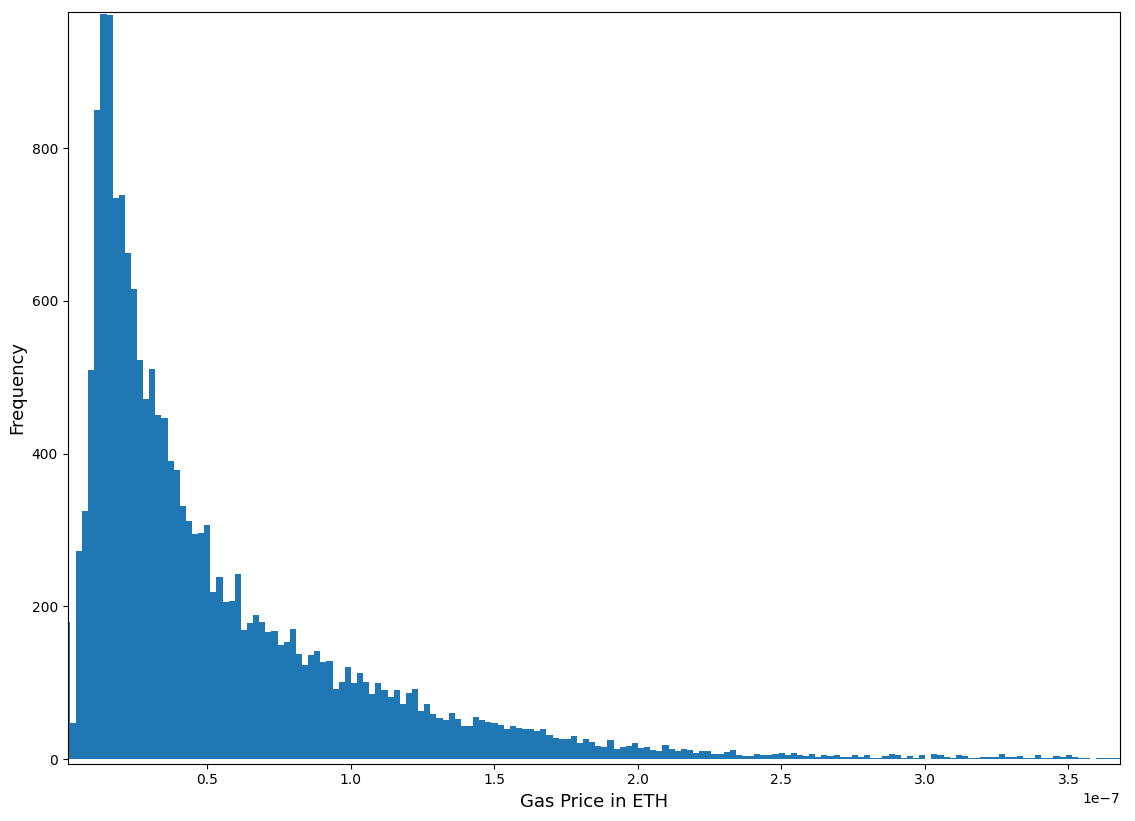
\includegraphics[width=0.7\linewidth]{evaluation/Images/GasPriceHistogram.png}
    \caption{Histogram Plot of Gas Prices in ETH}
    \label{fig:GasPriceHistogram}
\end{figure}
\\[3mm]
\noindent Therefore, our investigation consists of varying this threshold to see its effects on the returns of each strategy, using batched transactions and the same parameters used in the above experiment, the thresholds are set to the $60^{th}, 70^{th},80^{th},90^{th},100^{th}$ quantiles. Table \ref{tab:VaryGasPriceThresholds} displays the results of varying these thresholds. It can be seen that filtering more costly opportunities, expectedly, reduces the number of actionable; however, the higher thresholds also show that these opportunities are still just as if not more profitable. In addition, to this, Figure \ref{fig:VaryGasPriceThresholds} shows that a low threshold benefits the constant hedge ratio strategy most as with the low threshold, it has a slight loss, and as the threshold increases, the return using the strategy decreases. Whereas the returns are hindered with a lower threshold as many profitable opportunities are missed due to the overly low threshold, resulting in a reduction in the overall profitability of the trading strategy. The figure also shows how setting the threshold after the $90^{th}$ percentile does little to no effect on the return, giving a slightly positive impact on the Lagged strategy and a slight negative impact on the remaining. This is likely because there are only a few arbitrage opportunities to be present in such times when the gas price is high, thus having little impact. It is also interesting to see that the Lagged and the Kalman Filter strategies perform better by setting the threshold to the $90^{th}$ percentile compared to the $80^{th}$ percentile, whereas the other strategies perform worse.
\\[3mm]
Overall, the analysis of varying gas price thresholds reveals that adjusting the threshold level directly impacts the number of actionable opportunities and the resulting returns. Higher thresholds filter out less favourable opportunities while still maintaining profitability. However, it is crucial to strike a balance and avoid setting the threshold too low, which may lead to missed profitable opportunities. Hence, the threshold is set to the $90^{th}$ percentile to get the best balance for the following experiments.

\begin{figure}[H]
    \centering
    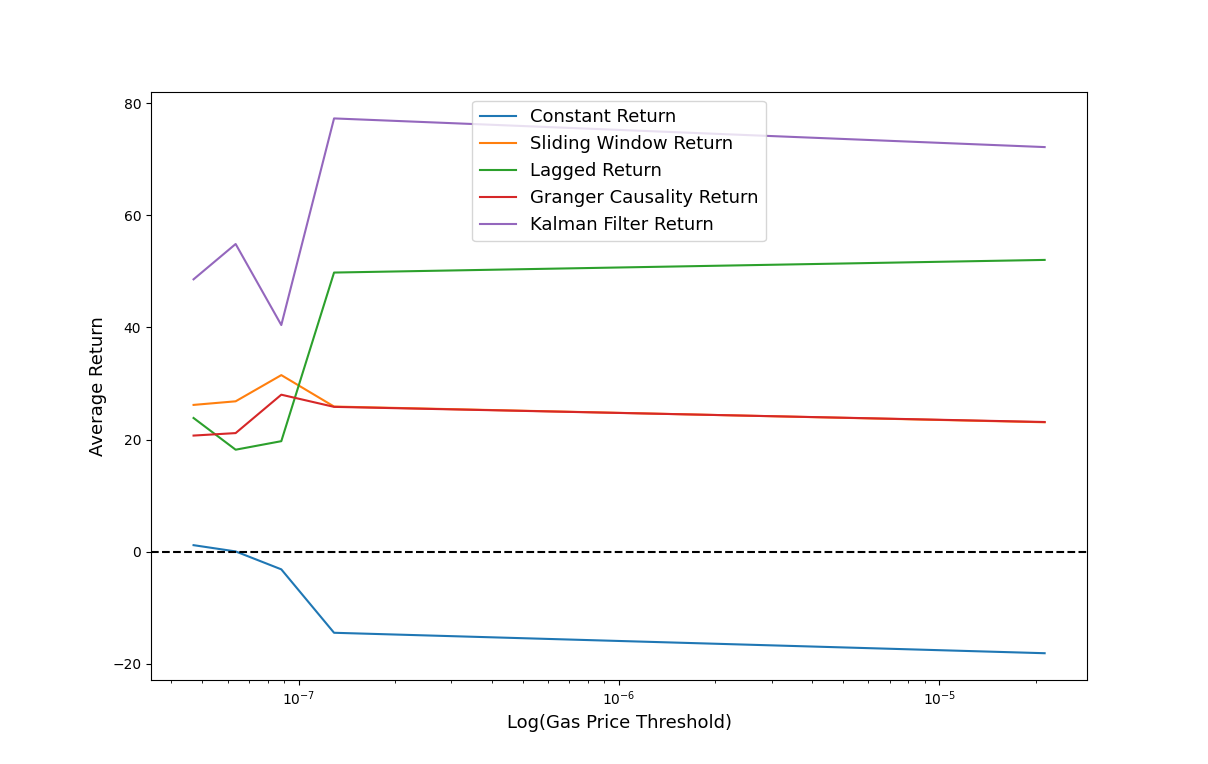
\includegraphics[width=\linewidth]{evaluation/Images/VaryGPThreshold.png}
    \caption{Average Returns of each strategy when using different gas price thresholds}
    \label{fig:VaryGasPriceThresholds}
\end{figure}

\begin{table}[htb!]
    \centering
    \begin{adjustwidth}{-0.9in}{-0.9in}
        \begin{tabular}{|p{5em}|p{2em}|p{3em}|p{3em}|p{3em}|p{3em}|p{3em}|p{3em}|p{3em}|p{3em}|p{3em}|p{3em}|}\hline
            Gas Price Threshold & Pool Pair & \multicolumn{10}{|c|}{Strategy's Annual Percentage Rate (APR) - Trading from 18th December 2021 to 9th June 2023} \\\cline{3-12}
            &   & \multicolumn{2}{|c|}{Constant} & \multicolumn{2}{|c|}{Sliding Window} & \multicolumn{2}{|c|}{Lagged} & \multicolumn{2}{|c|}{Granger Causality} & \multicolumn{2}{|c|}{Kalman Filter}\\\cline{3-12}
            & & Return \% & \# of Trades & Return \% & \# of Trades & Return \% & \# of Trades & Return \% & \# of Trades & Return \% & \# of Trades\\\hline

            & 0 & \textcolor{green}{7.97} & 193 & \textcolor{green}{26.18} & 221 & \textcolor{green}{30.36} & 242 & \textcolor{green}{30.83} & 124 & \textcolor{green}{51.35} & 105\\\cline{3-12}
            & 1 & \textcolor{red}{-23.52} & 253 & \textcolor{red}{-0.69} & 178 & \textcolor{red}{-9.49} & 205 & \textcolor{green}{7.4} & 139 & \textcolor{green}{26.12} & 124\\\cline{3-12}
            & 2 & \textcolor{green}{8.71} & 134 & \textcolor{green}{30.05} & 171 & \textcolor{green}{26.33} & 169 & \textcolor{green}{30.82} & 103 & \textcolor{green}{51.46} & 77\\\cline{3-12}
            $60^{th}$ percentile = 4.7e-08 & 3 & \textcolor{red}{-22.44} & 214 & \textcolor{green}{0.58} & 165 & \textcolor{red}{-8.34} & 188 & \textcolor{green}{7.65} & 134 & \textcolor{green}{31.41} & 90\\[-5.5ex]\cline{3-12}
            & 4 & \textcolor{green}{14.69} & 150 & \textcolor{green}{34.45} & 178 & \textcolor{green}{24.69} & 184 & \textcolor{green}{31.4} & 123 & \textcolor{green}{47.09} & 90\\\cline{3-12}
            & 5 & \textcolor{red}{-12.54} & 191 & \textcolor{green}{6.98} & 128 & \textcolor{green}{3.85} & 150 & \textcolor{green}{15.33} & 124 & \textcolor{green}{38.32} & 96\\\cline{3-12}
            & 6 & \textcolor{red}{-27.3} & 53 & \textcolor{red}{-4.83} & 30 & \textcolor{red}{-15.56} & 46 & \textcolor{red}{-25.36} & 26 & \textcolor{red}{-6.35} & 50\\\hline\hline

            & 0 & \textcolor{green}{12.85} & 216 & \textcolor{green}{33.49} & 255 & \textcolor{green}{33.74} & 277 & \textcolor{green}{33.2} & 146 & \textcolor{green}{58.28} & 120\\\cline{3-12}
            & 1 & \textcolor{red}{-24.53} & 283 & \textcolor{red}{-2.14} & 209 & \textcolor{red}{-17.44} & 243 & \textcolor{green}{4.14} & 161 & \textcolor{green}{29.83} & 140\\\cline{3-12}
            & 2 & \textcolor{green}{12.4} & 156 & \textcolor{green}{33.28} & 199 & \textcolor{green}{25.97} & 200 & \textcolor{green}{36.35} & 123 & \textcolor{green}{61.2} & 94\\\cline{3-12}
            $70^{th}$ percentile = 6.36e-08 & 3 & \textcolor{red}{-23.07} & 240 & \textcolor{green}{0.35} & 193 & \textcolor{red}{-14.67} & 219 & \textcolor{green}{4.35} & 162 & \textcolor{green}{35.85} & 107\\[-5.5ex]\cline{3-12}
            & 4 & \textcolor{green}{14.6} & 175 & \textcolor{green}{33.64} & 215 & \textcolor{green}{23.48} & 219 & \textcolor{green}{38.4} & 152 & \textcolor{green}{59.88} & 111\\\cline{3-12}
            & 5 & \textcolor{red}{-13.43} & 220 & \textcolor{green}{6.63} & 152 & \textcolor{red}{-3.77} & 179 & \textcolor{green}{13.97} & 148 & \textcolor{green}{42.8} & 116\\\cline{3-12}
            & 6 & \textcolor{red}{-26.12} & 59 & \textcolor{red}{-6.02} & 37 & \textcolor{red}{-17.86} & 56 & \textcolor{red}{-17.84} & 30 & \textcolor{red}{-8.94} & 58\\\hline\hline

            & 0 & \textcolor{green}{12.79} & 239 & \textcolor{green}{37.89} & 282 & \textcolor{green}{42.17} & 298 & \textcolor{green}{55.47} & 159 & \textcolor{green}{48.36} & 127\\\cline{3-12}
            & 1 & \textcolor{red}{-27.28} & 310 & \textcolor{red}{-3.55} & 235 & \textcolor{red}{-17.09} & 267 & \textcolor{green}{17.17} & 178 & \textcolor{green}{19.48} & 148\\\cline{3-12}
            & 2 & \textcolor{green}{12.72} & 182 & \textcolor{green}{37.34} & 224 & \textcolor{green}{34.2} & 222 & \textcolor{green}{63.04} & 141 & \textcolor{green}{50.22} & 102\\\cline{3-12}
            $80^{th}$ percentile = 8.83e-08 & 3 & \textcolor{red}{-27.36} & 266 & \textcolor{red}{-1.32} & 220 & \textcolor{red}{-14.55} & 247 & \textcolor{green}{14.51} & 177 & \textcolor{green}{24.88} & 116\\[-5.5ex]\cline{3-12}
            & 4 & \textcolor{green}{14.38} & 196 & \textcolor{green}{37.34} & 241 & \textcolor{green}{30.37} & 240 & \textcolor{green}{63.65} & 164 & \textcolor{green}{50.73} & 122\\\cline{3-12}
            & 5 & \textcolor{red}{-14.74} & 239 & \textcolor{green}{8.61} & 177 & \textcolor{red}{-3.93} & 201 & \textcolor{green}{25.26} & 162 & \textcolor{green}{32.34} & 123\\\cline{3-12}
            & 6 & \textcolor{red}{-25.48} & 60 & \textcolor{red}{-12.8} & 46 & \textcolor{red}{-16.09} & 59 & \textcolor{red}{-16.77} & 32 & \textcolor{red}{-8.39} & 59\\\hline\hline

            & 0 & \textcolor{green}{7.19} & 261 & \textcolor{green}{35.32} & 307 & \textcolor{green}{89.98} & 323 & \textcolor{green}{52.91} & 176 & \textcolor{green}{82.2} & 146\\\cline{3-12}
            & 1 & \textcolor{red}{-40.49} & 336 & \textcolor{red}{-9.77} & 264 & \textcolor{green}{5.2} & 294 & \textcolor{green}{10.93} & 197 & \textcolor{green}{40.46} & 167\\\cline{3-12}
            & 2 & \textcolor{green}{5.12} & 201 & \textcolor{green}{31.92} & 249 & \textcolor{green}{73.17} & 244 & \textcolor{green}{63.31} & 161 & \textcolor{green}{80.48} & 122\\\cline{3-12}
            $90^{th}$ percentile = 1.29e-07 & 3 & \textcolor{red}{-34.87} & 287 & \textcolor{red}{-6.13} & 243 & \textcolor{green}{7.72} & 272 & \textcolor{green}{15.23} & 195 & \textcolor{green}{46.48} & 133\\[-5.5ex]\cline{3-12}
            & 4 & \textcolor{green}{8.38} & 217 & \textcolor{green}{32.28} & 267 & \textcolor{green}{66.24} & 264 & \textcolor{green}{58.31} & 187 & \textcolor{green}{82.52} & 139\\\cline{3-12}
            & 5 & \textcolor{red}{-29.62} & 265 & \textcolor{red}{-0.58} & 201 & \textcolor{green}{22.09} & 226 & \textcolor{green}{20.87} & 183 & \textcolor{green}{55.01} & 144\\\cline{3-12}
            & 6 & \textcolor{red}{-30.43} & 69 & \textcolor{red}{-15.39} & 56 & \textcolor{red}{-18.0} & 70 & \textcolor{red}{-18.27} & 34 & \textcolor{red}{-9.18} & 67\\\hline\hline

            & 0 & \textcolor{red}{-2.2} & 288 & \textcolor{green}{30.8} & 342 & \textcolor{green}{87.79} & 353 & \textcolor{green}{66.76} & 192 & \textcolor{green}{100.13} & 153\\\cline{3-12}
            & 1 & \textcolor{red}{-47.23} & 358 & \textcolor{red}{-16.28} & 293 & \textcolor{green}{0.91} & 323 & \textcolor{green}{16.58} & 213 & \textcolor{green}{46.78} & 178\\\cline{3-12}
            & 2 & \textcolor{green}{2.63} & 225 & \textcolor{green}{28.29} & 277 & \textcolor{green}{74.07} & 270 & \textcolor{green}{75.52} & 180 & \textcolor{green}{97.43} & 133\\\cline{3-12}
            $100^{th}$ percentile = 2.13e-05 & 3 & \textcolor{red}{-42.06} & 309 & \textcolor{red}{-9.95} & 268 & \textcolor{green}{4.71} & 294 & \textcolor{green}{25.33} & 211 & \textcolor{green}{52.93} & 145\\[-5.5ex]\cline{3-12}
            & 4 & \textcolor{green}{1.72} & 241 & \textcolor{green}{29.97} & 294 & \textcolor{green}{62.84} & 291 & \textcolor{green}{69.21} & 201 & \textcolor{green}{86.18} & 152\\\cline{3-12}
            & 5 & \textcolor{red}{-37.04} & 287 & \textcolor{red}{-4.83} & 225 & \textcolor{green}{14.37} & 250 & \textcolor{green}{23.51} & 200 & \textcolor{green}{62.31} & 152\\\cline{3-12}
            & 6 & \textcolor{red}{-33.66} & 76 & \textcolor{red}{-17.93} & 67 & \textcolor{red}{-27.78} & 76 & \textcolor{red}{-21.93} & 37 & \textcolor{red}{-14.77} & 74\\\hline
        \end{tabular}
    \end{adjustwidth}
    \caption{Returns of each strategy when using different gas price thresholds \label{tab:VaryGasPriceThresholds}}.
\end{table}

\subsection{Initial Investment Volume}
Another important factor contributing to the profit is the initial investment; therefore, Table \ref{tab:VaryInitialInvestments} and Figure \ref{fig:VaryInitialInvestments} display the returns of various initial investments. It can immediately be seen that the higher the investment, the greater the return. However, the smallest investments fall to a loss immediately for all strategies because the fee incurred by gas fees is fixed regardless of the volume. In contrast, the costs incurred by Aave and Uniswap are proportional to the volume being traded. This fixed fee means that a greater volume is required to cover the cost of the gas fee in order to generate profit, which is, of course, proportional to the volume being traded. Hence, as the investment increases, the return increases; however, it begins to plateau after 25ETH as the fixed fee becomes negligible compared to the investment.
\\[3mm]
Upon comparing the different strategies, the Kalman Filter can generate a profit with the least investment, followed by the Granger Causality strategy, then the Lagged and Sliding Window strategies and finally, the Constant strategy fails to make any money with any investment. Interestingly, although the Granger Causality test strategy can churn a better return at lower initial investments, when initial investment $\leq 20$, the Lagged strategy overtakes the returns of the Granger Causality strategy once returns hit 0\%. The Lagged strategy plateaus to around 60\% whereas the Granger Causality strategy plateaus to 50\%, indicating that although both of these methods assess the causality of the price dynamic between the two liquidity pairs, the lagged strategy estimates the hedge ratio better than the unrestricted model generated from the Granger Causality test.

\begin{figure}[H]
    \centering
    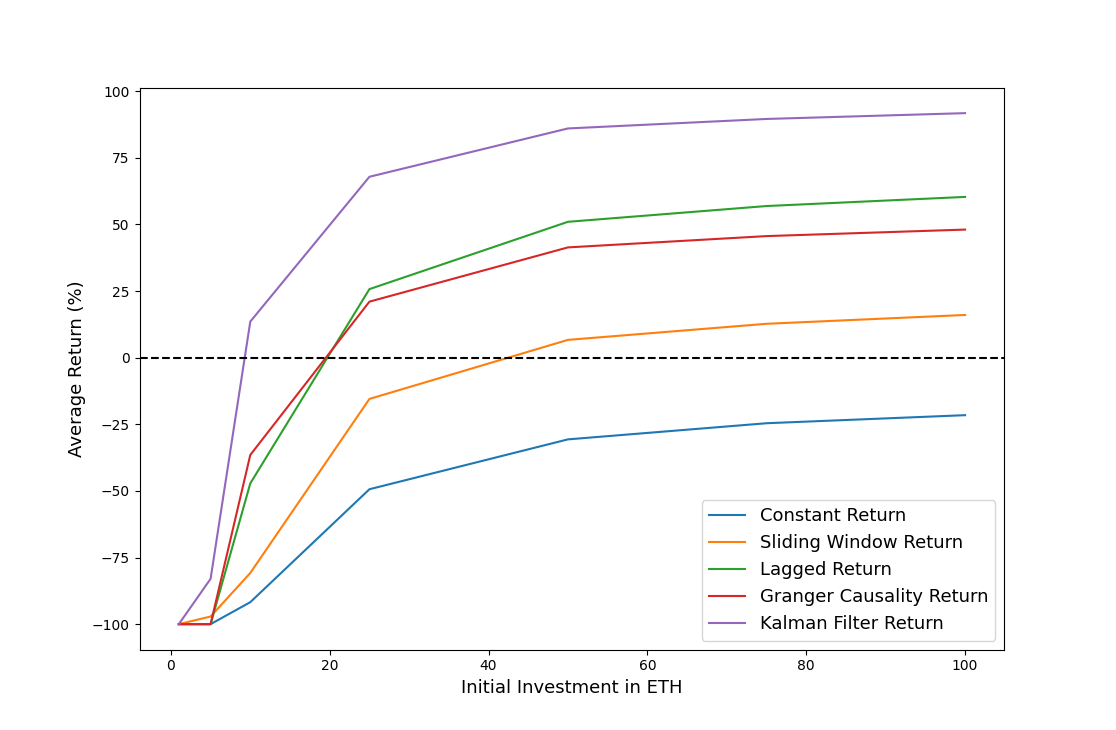
\includegraphics[width=\linewidth]{evaluation/Images/VaryII.png}
    \caption{Average Returns of each strategy using different initial investment volumes}
    \label{fig:VaryInitialInvestments}
\end{figure}

\begin{table}[htb!]
    \centering
    \begin{adjustwidth}{-0.9in}{-0.9in}
        \begin{tabular}{|p{5em}|p{2em}|p{3em}|p{3em}|p{3em}|p{3em}|p{3em}|p{3em}|p{3em}|p{3em}|p{3em}|p{3em}|}\hline
            Initial Investment & Pool Pair & \multicolumn{10}{|c|}{Strategy's Annual Percentage Rate (APR) - Trading from 18th December 2021 to 9th June 2023} \\\cline{3-12}
            &   & \multicolumn{2}{|c|}{Constant} & \multicolumn{2}{|c|}{Sliding Window} & \multicolumn{2}{|c|}{Lagged} & \multicolumn{2}{|c|}{Granger Causality} & \multicolumn{2}{|c|}{Kalman Filter}\\\cline{3-12}
            & & Return \% & \# of Trades & Return \% & \# of Trades & Return \% & \# of Trades & Return \% & \# of Trades & Return \% & \# of Trades\\\hline

            & 0 & \textcolor{red}{-100.0} & 3 & \textcolor{red}{-100.0} & 4 & \textcolor{red}{-100.0} & 2 & \textcolor{red}{-100.0} & 2 & \textcolor{red}{-100.0} & 3\\\cline{3-12}
            & 1 & \textcolor{red}{-100.0} & 3 & \textcolor{red}{-100.0} & 4 & \textcolor{red}{-100.0} & 2 & \textcolor{red}{-100.0} & 2 & \textcolor{red}{-100.0} & 3\\\cline{3-12}
            & 2 & \textcolor{red}{-100.0} & 3 & \textcolor{red}{-100.0} & 4 & \textcolor{red}{-100.0} & 2 & \textcolor{red}{-100.0} & 3 & \textcolor{red}{-100.0} & 3\\\cline{3-12}
            $1 ETH = \$3,946.26$ & 3 & \textcolor{red}{-100.0} & 3 & \textcolor{red}{-100.0} & 4 & \textcolor{red}{-100.0} & 2 & \textcolor{red}{-100.0} & 3 & \textcolor{red}{-100.0} & 3\\[-3ex]\cline{3-12}
            & 4 & \textcolor{red}{-100.0} & 3 & \textcolor{red}{-100.0} & 4 & \textcolor{red}{-100.0} & 2 & \textcolor{red}{-100.0} & 4 & \textcolor{red}{-100.0} & 3\\\cline{3-12}
            & 5 & \textcolor{red}{-100.0} & 3 & \textcolor{red}{-100.0} & 5 & \textcolor{red}{-100.0} & 2 & \textcolor{red}{-100.0} & 2 & \textcolor{red}{-100.0} & 3\\\cline{3-12}
            & 6 & \textcolor{red}{-100.0} & 4 & \textcolor{red}{-100.0} & 3 & \textcolor{red}{-100.0} & 2 & \textcolor{red}{-100.0} & 2 & \textcolor{red}{-100.0} & 2\\\hline\hline
            & 0 & \textcolor{red}{-100.0} & 72 & \textcolor{red}{-100.0} & 133 & \textcolor{red}{-100.0} & 226 & \textcolor{red}{-100.0} & 144 & \textcolor{red}{-92.99} & 146\\\cline{3-12}
            & 1 & \textcolor{red}{-100.0} & 67 & \textcolor{red}{-100.0} & 104 & \textcolor{red}{-100.0} & 162 & \textcolor{red}{-100.0} & 30 & \textcolor{red}{-100.0} & 160\\\cline{3-12}
            & 2 & \textcolor{red}{-100.0} & 79 & \textcolor{red}{-100.0} & 138 & \textcolor{red}{-100.0} & 199 & \textcolor{red}{-100.0} & 132 & \textcolor{red}{-87.15} & 122\\\cline{3-12}
            $5 ETH = \$19,731.30$ & 3 & \textcolor{red}{-100.0} & 71 & \textcolor{red}{-100.0} & 135 & \textcolor{red}{-100.0} & 165 & \textcolor{red}{-100.0} & 112 & \textcolor{red}{-100.0} & 121\\[-3ex]\cline{3-12}
            & 4 & \textcolor{red}{-100.0} & 63 & \textcolor{red}{-100.0} & 135 & \textcolor{red}{-100.0} & 174 & \textcolor{red}{-100.0} & 129 & \textcolor{red}{-88.55} & 139\\\cline{3-12}
            & 5 & \textcolor{red}{-100.0} & 67 & \textcolor{red}{-100.0} & 114 & \textcolor{red}{-100.0} & 147 & \textcolor{red}{-100.0} & 100 & \textcolor{red}{-97.5} & 144\\\cline{3-12}
            & 6 & \textcolor{red}{-100.0} & 37 & \textcolor{red}{-96.31} & 56 & \textcolor{red}{-100.0} & 70 & \textcolor{red}{-100.0} & 8 & \textcolor{red}{-100.0} & 35\\\hline\hline
            & 0 & \textcolor{red}{-100.0} & 241 & \textcolor{red}{-73.29} & 307 & \textcolor{red}{-5.49} & 323 & \textcolor{red}{-9.44} & 176 & \textcolor{green}{28.26} & 146\\\cline{3-12}
            & 1 & \textcolor{red}{-100.0} & 216 & \textcolor{red}{-100.0} & 227 & \textcolor{red}{-100.0} & 291 & \textcolor{red}{-56.99} & 197 & \textcolor{red}{-7.98} & 167\\\cline{3-12}
            & 2 & \textcolor{red}{-72.85} & 201 & \textcolor{red}{-55.37} & 249 & \textcolor{red}{-3.76} & 244 & \textcolor{red}{-1.41} & 161 & \textcolor{green}{28.45} & 122\\\cline{3-12}
            $10 ETH = \$39,462.60$ & 3 & \textcolor{red}{-100.0} & 231 & \textcolor{red}{-100.0} & 240 & \textcolor{red}{-73.99} & 272 & \textcolor{red}{-50.8} & 195 & \textcolor{green}{1.99} & 133\\[-3ex]\cline{3-12}
            & 4 & \textcolor{red}{-80.04} & 217 & \textcolor{red}{-64.22} & 267 & \textcolor{red}{-14.27} & 264 & \textcolor{red}{-11.29} & 187 & \textcolor{green}{30.22} & 139\\\cline{3-12}
            & 5 & \textcolor{red}{-100.0} & 221 & \textcolor{red}{-75.2} & 201 & \textcolor{red}{-48.32} & 226 & \textcolor{red}{-42.44} & 183 & \textcolor{green}{6.61} & 144\\\cline{3-12}
            & 6 & \textcolor{red}{-52.11} & 69 & \textcolor{red}{-37.11} & 56 & \textcolor{red}{-42.18} & 70 & \textcolor{red}{-35.21} & 34 & \textcolor{red}{-30.05} & 67\\\hline\hline

            & 0 & \textcolor{red}{-18.93} & 261 & \textcolor{green}{7.87} & 307 & \textcolor{green}{62.82} & 323 & \textcolor{green}{33.34} & 176 & \textcolor{green}{67.25} & 146\\\cline{3-12}
            & 1 & \textcolor{red}{-71.42} & 336 & \textcolor{red}{-33.85} & 264 & \textcolor{red}{-17.26} & 294 & \textcolor{red}{-5.83} & 197 & \textcolor{green}{28.16} & 167\\\cline{3-12}
            & 2 & \textcolor{red}{-15.96} & 201 & \textcolor{green}{7.51} & 249 & \textcolor{green}{49.6} & 244 & \textcolor{green}{45.58} & 161 & \textcolor{green}{66.77} & 122\\\cline{3-12}
            $25 ETH = \$98,656.50$ & 3 & \textcolor{red}{-58.44} & 287 & \textcolor{red}{-26.86} & 243 & \textcolor{red}{-12.37} & 272 & \textcolor{red}{-3.11} & 195 & \textcolor{green}{32.29} & 133\\[-3ex]\cline{3-12}
            & 4 & \textcolor{red}{-15.09} & 217 & \textcolor{green}{6.05} & 267 & \textcolor{green}{42.03} & 264 & \textcolor{green}{37.49} & 187 & \textcolor{green}{65.93} & 139\\\cline{3-12}
            & 5 & \textcolor{red}{-53.22} & 265 & \textcolor{red}{-19.49} & 201 & \textcolor{green}{2.9} & 226 & \textcolor{green}{4.43} & 183 & \textcolor{green}{40.5} & 144\\\cline{3-12}
            & 6 & \textcolor{red}{-38.19} & 69 & \textcolor{red}{-22.01} & 56 & \textcolor{red}{-26.43} & 70 & \textcolor{red}{-24.02} & 34 & \textcolor{red}{-15.81} & 67\\\hline\hline

            & 0 & \textcolor{red}{-0.76} & 261 & \textcolor{green}{27.61} & 307 & \textcolor{green}{82.45} & 323 & \textcolor{green}{48.52} & 176 & \textcolor{green}{78.51} & 146\\\cline{3-12}
            & 1 & \textcolor{red}{-49.33} & 336 & \textcolor{red}{-16.59} & 264 & \textcolor{red}{-1.54} & 294 & \textcolor{green}{6.43} & 197 & \textcolor{green}{37.68} & 167\\\cline{3-12}
            & 2 & \textcolor{red}{-1.27} & 201 & \textcolor{green}{25.19} & 249 & \textcolor{green}{67.31} & 244 & \textcolor{green}{59.25} & 161 & \textcolor{green}{77.32} & 122\\\cline{3-12}
            $50 ETH = \$197,313.00$ & 3 & \textcolor{red}{-41.96} & 287 & \textcolor{red}{-11.83} & 243 & \textcolor{green}{3.3} & 272 & \textcolor{green}{10.75} & 195 & \textcolor{green}{43.43} & 133\\[-3ex]\cline{3-12}
            & 4 & \textcolor{green}{0.85} & 217 & \textcolor{green}{25.11} & 267 & \textcolor{green}{59.95} & 264 & \textcolor{green}{53.16} & 187 & \textcolor{green}{78.63} & 139\\\cline{3-12}
            & 5 & \textcolor{red}{-37.12} & 265 & \textcolor{red}{-6.58} & 201 & \textcolor{green}{17.6} & 226 & \textcolor{green}{17.37} & 183 & \textcolor{green}{51.84} & 144\\\cline{3-12}
            & 6 & \textcolor{red}{-33.3} & 69 & \textcolor{red}{-17.81} & 56 & \textcolor{red}{-20.8} & 70 & \textcolor{red}{-20.18} & 34 & \textcolor{red}{-11.58} & 67\\\hline\hline

            & 0 & \textcolor{green}{4.54} & 261 & \textcolor{green}{32.75} & 307 & \textcolor{green}{87.19} & 323 & \textcolor{green}{51.42} & 176 & \textcolor{green}{80.97} & 146\\\cline{3-12}
            & 1 & \textcolor{red}{-43.77} & 336 & \textcolor{red}{-12.39} & 264 & \textcolor{green}{2.51} & 294 & \textcolor{green}{9.31} & 197 & \textcolor{green}{39.03} & 167\\\cline{3-12}
            & 2 & \textcolor{green}{2.97} & 201 & \textcolor{green}{29.4} & 249 & \textcolor{green}{70.56} & 244 & \textcolor{green}{61.79} & 161 & \textcolor{green}{79.32} & 122\\\cline{3-12}
            $75 ETH = \$295,969.50$ & 3 & \textcolor{red}{-37.01} & 287 & \textcolor{red}{-8.16} & 243 & \textcolor{green}{6.7} & 272 & \textcolor{green}{13.5} & 195 & \textcolor{green}{45.19} & 133\\[-3ex]\cline{3-12}
            & 4 & \textcolor{green}{6.18} & 217 & \textcolor{green}{29.66} & 267 & \textcolor{green}{64.16} & 264 & \textcolor{green}{56.71} & 187 & \textcolor{green}{81.31} & 139\\\cline{3-12}
            & 5 & \textcolor{red}{-32.1} & 265 & \textcolor{red}{-2.36} & 201 & \textcolor{green}{20.4} & 226 & \textcolor{green}{19.21} & 183 & \textcolor{green}{53.72} & 144\\\cline{3-12}
            & 6 & \textcolor{red}{-31.37} & 69 & \textcolor{red}{-16.19} & 56 & \textcolor{red}{-18.93} & 70 & \textcolor{red}{-18.9} & 34 & \textcolor{red}{-9.98} & 67\\\hline\hline

            & 0 & \textcolor{green}{7.19} & 261 & \textcolor{green}{35.32} & 307 & \textcolor{green}{89.98} & 323 & \textcolor{green}{52.91} & 176 & \textcolor{green}{82.2} & 146\\\cline{3-12}
            & 1 & \textcolor{red}{-40.49} & 336 & \textcolor{red}{-9.77} & 264 & \textcolor{green}{5.2} & 294 & \textcolor{green}{10.93} & 197 & \textcolor{green}{40.46} & 167\\\cline{3-12}
            & 2 & \textcolor{green}{5.12} & 201 & \textcolor{green}{31.92} & 249 & \textcolor{green}{73.17} & 244 & \textcolor{green}{63.31} & 161 & \textcolor{green}{80.48} & 122\\\cline{3-12}
            $100 ETH = \$394,626.00$ & 3 & \textcolor{red}{-34.87} & 287 & \textcolor{red}{-6.13} & 243 & \textcolor{green}{7.72} & 272 & \textcolor{green}{15.23} & 195 & \textcolor{green}{46.48} & 133\\[-3ex]\cline{3-12}
            & 4 & \textcolor{green}{8.38} & 217 & \textcolor{green}{32.28} & 267 & \textcolor{green}{66.24} & 264 & \textcolor{green}{58.31} & 187 & \textcolor{green}{82.52} & 139\\\cline{3-12}
            & 5 & \textcolor{red}{-29.62} & 265 & \textcolor{red}{-0.58} & 201 & \textcolor{green}{22.09} & 226 & \textcolor{green}{20.87} & 183 & \textcolor{green}{55.01} & 144\\\cline{3-12}
            & 6 & \textcolor{red}{-30.43} & 69 & \textcolor{red}{-15.39} & 56 & \textcolor{red}{-18.0} & 70 & \textcolor{red}{-18.27} & 34 & \textcolor{red}{-9.18} & 67\\\hline
        \end{tabular}
    \end{adjustwidth}
    \caption{Returns of each strategy when using different initial investment volumes (Note: Ethereum to USD conversion rate is from 18th December 2021) \label{tab:VaryInitialInvestments}}.
\end{table}

\subsection{Window Size}
The final parameter that also affects the returns is the window size. This window size is used when calculating the mean and standard deviation to calculate the thresholds. As we can see in the excerpt below, the greater the window size, the more data the strategy would use to calculate the thresholds.
\vspace{5mm}
\begin{lstlisting}[language=Python]
spread = self.history_p1[-self.window_size_in_hours:] - self.hedge_ratio * self.history_p2[-self.window_size_in_hours:]
spread_mean = spread.mean()
spread_std = spread.std()
self.upper_threshold = spread_mean + self.number_of_sds_from_mean * spread_std
self.lower_threshold = spread_mean - self.number_of_sds_from_mean * spread_std
\end{lstlisting}
\vspace{5mm}
To evaluate how the window size affects the returns, backtesting is conducted from 9th June 2022 to the 9th June 2023, exactly 1 year. The results can be found in Table \ref{tab:VaryWS} and Figure \ref{fig:VaryWS} where we can see that, as the window sizes increase, the returns increase; however, for the smaller window sizes, the return are more erratic and volatile. This volatility decreases as the window size increases, plateauing to each strategy's returns.
\\[3mm]
It is also interesting to see that in this period of trading, the Kalman Filter performs the worst, which is surprising as it has outperformed each of the strategies in the experiment that have been previously mentioned.

\begin{figure}[H]
    \centering
    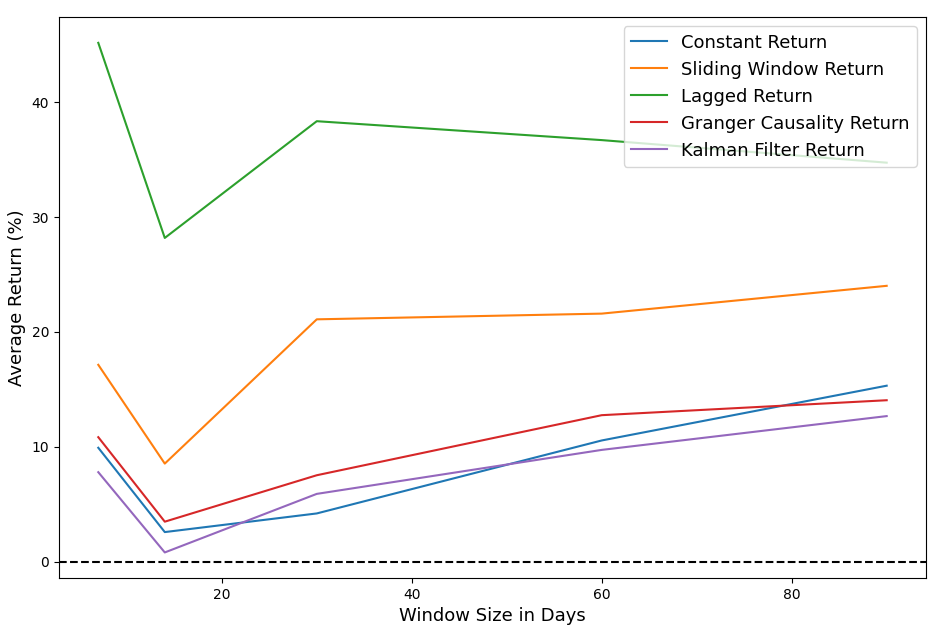
\includegraphics[width=\linewidth]{evaluation/Images/VarWS.png}
    \caption{Average Returns of each strategy using different Window Sizes}
    \label{fig:VaryWS}
\end{figure}

\begin{table}[!htb]
    \centering
    \begin{adjustwidth}{-0.8in}{-0.9in}
        \begin{tabular}{|p{4em}|p{2em}|p{3em}|p{3em}|p{3em}|p{3em}|p{3em}|p{3em}|p{3em}|p{3em}|p{3em}|p{3em}|}\hline
            Window Size & Pool Pair & \multicolumn{10}{|c|}{Strategy's Annual Percentage Rate (APR) - Trading from 9th June 2022 to the 9th June 2023} \\\cline{3-12}
            &   & \multicolumn{2}{|c|}{Constant} & \multicolumn{2}{|c|}{Sliding Window} & \multicolumn{2}{|c|}{Lagged} & \multicolumn{2}{|c|}{Granger Causality} & \multicolumn{2}{|c|}{Kalman Filter}\\\cline{3-12}
            & & Return \% & \# of Trades & Return \% & \# of Trades & Return \% & \# of Trades & Return \% & \# of Trades & Return \% & \# of Trades\\\hline

            & 0 & \textcolor{green}{22.15} & 404 & \textcolor{green}{51.04} & 329 & \textcolor{green}{35.35} & 357 & \textcolor{green}{76.7} & 238 & \textcolor{green}{24.5} & 358\\\cline{3-12}
            & 1 & \textcolor{red}{-36.93} & 328 & \textcolor{red}{-11.1} & 273 & \textcolor{red}{-28.35} & 304 & \textcolor{red}{-1.24} & 316 & \textcolor{red}{-26.28} & 293\\\cline{3-12}
            & 2 & \textcolor{green}{21.97} & 365 & \textcolor{green}{46.2} & 336 & \textcolor{green}{36.53} & 332 & \textcolor{green}{81.15} & 234 & \textcolor{green}{15.32} & 362\\\cline{3-12}
            7 days & 3 & \textcolor{red}{-37.98} & 323 & \textcolor{red}{-18.41} & 278 & \textcolor{red}{-27.55} & 293 & \textcolor{red}{-8.08} & 315 & \textcolor{red}{-35.33} & 306\\\cline{3-12}
            & 4 & \textcolor{green}{26.56} & 377 & \textcolor{green}{44.91} & 351 & \textcolor{green}{40.59} & 344 & \textcolor{green}{83.15} & 255 & \textcolor{green}{23.02} & 334\\\cline{3-12}
            & 5 & \textcolor{red}{-26.07} & 272 & \textcolor{red}{-6.36} & 231 & \textcolor{red}{-21.73} & 249 & \textcolor{green}{15.63} & 268 & \textcolor{red}{-21.63} & 239\\\cline{3-12}
            & 6 & \textcolor{red}{-28.77} & 63 & \textcolor{red}{-21.75} & 67 & \textcolor{red}{-23.42} & 65 & \textcolor{red}{-15.56} & 31 & \textcolor{red}{-27.23} & 67\\\hline\hline

            & 0 & \textcolor{green}{20.66} & 383 & \textcolor{green}{11.37} & 293 & \textcolor{green}{15.97} & 352 & \textcolor{green}{40.32} & 182 & \textcolor{green}{10.84} & 353\\\cline{3-12}
            & 1 & \textcolor{red}{-31.35} & 318 & \textcolor{red}{-24.58} & 249 & \textcolor{red}{-38.7} & 287 & \textcolor{red}{-15.16} & 246 & \textcolor{red}{-34.38} & 277\\\cline{3-12}
            & 2 & \textcolor{green}{17.73} & 327 & \textcolor{green}{10.61} & 283 & \textcolor{green}{5.99} & 311 & \textcolor{green}{38.21} & 186 & \textcolor{green}{6.87} & 311\\\cline{3-12}
            14 days & 3 & \textcolor{red}{-29.1} & 299 & \textcolor{red}{-35.08} & 268 & \textcolor{red}{-40.28} & 297 & \textcolor{red}{-20.64} & 256 & \textcolor{red}{-43.54} & 312\\\cline{3-12}
            & 4 & \textcolor{green}{20.21} & 346 & \textcolor{green}{11.44} & 278 & \textcolor{green}{5.44} & 308 & \textcolor{green}{47.6} & 212 & \textcolor{green}{12.56} & 305\\\cline{3-12}
            & 5 & \textcolor{red}{-18.27} & 251 & \textcolor{red}{-13.4} & 192 & \textcolor{red}{-29.71} & 242 & \textcolor{red}{-8.71} & 200 & \textcolor{red}{-28.11} & 231\\\cline{3-12}
            & 6 & \textcolor{red}{-24.32} & 42 & \textcolor{red}{-17.15} & 45 & \textcolor{red}{-5.46} & 38 & \textcolor{red}{-38.92} & 32 & \textcolor{red}{-19.27} & 45\\\hline\hline

            & 0 & \textcolor{green}{21.69} & 289 & \textcolor{green}{39.05} & 260 & \textcolor{green}{75.61} & 270 & \textcolor{green}{55.53} & 104 & \textcolor{green}{10.56} & 323\\\cline{3-12}
            & 1 & \textcolor{red}{-32.04} & 318 & \textcolor{red}{-9.96} & 219 & \textcolor{red}{-4.39} & 238 & \textcolor{green}{21.46} & 133 & \textcolor{red}{-42.09} & 287\\\cline{3-12}
            & 2 & \textcolor{green}{19.44} & 208 & \textcolor{green}{39.02} & 203 & \textcolor{green}{66.67} & 193 & \textcolor{green}{57.53} & 85 & \textcolor{green}{3.43} & 232\\\cline{3-12}
            30 days & 3 & \textcolor{red}{-26.53} & 274 & \textcolor{red}{-7.43} & 200 & \textcolor{green}{0.83} & 219 & \textcolor{green}{24.28} & 117 & \textcolor{red}{-39.38} & 241\\\cline{3-12}
            & 4 & \textcolor{green}{15.11} & 245 & \textcolor{green}{36.06} & 217 & \textcolor{green}{52.06} & 206 & \textcolor{green}{60.94} & 104 & \textcolor{green}{8.39} & 257\\\cline{3-12}
            & 5 & \textcolor{red}{-12.89} & 214 & \textcolor{green}{2.11} & 153 & \textcolor{green}{14.63} & 168 & \textcolor{green}{35.09} & 105 & \textcolor{red}{-30.14} & 218\\\cline{3-12}
            & 6 & \textcolor{red}{-9.55} & 24 & \textcolor{green}{0.45} & 26 & \textcolor{green}{11.62} & 16 & \textcolor{red}{-23.8} & 21 & \textcolor{red}{-5.29} & 24\\\hline\hline

            & 0 & \textcolor{green}{15.48} & 314 & \textcolor{green}{48.26} & 275 & \textcolor{green}{68.23} & 277 & \textcolor{green}{81.41} & 108 & \textcolor{green}{21.07} & 351\\\cline{3-12}
            & 1 & \textcolor{red}{-28.11} & 303 & \textcolor{red}{-0.49} & 180 & \textcolor{green}{20.55} & 172 & \textcolor{green}{42.31} & 135 & \textcolor{red}{-34.98} & 259\\\cline{3-12}
            & 2 & \textcolor{green}{22.46} & 100 & \textcolor{green}{40.3} & 92 & \textcolor{green}{67.59} & 83 & \textcolor{green}{77.2} & 50 & \textcolor{green}{13.71} & 147\\\cline{3-12}
            60 days & 3 & \textcolor{red}{-6.78} & 179 & \textcolor{green}{13.53} & 112 & \textcolor{green}{39.52} & 96 & \textcolor{green}{56.05} & 68 & \textcolor{red}{-22.18} & 154\\\cline{3-12}
            & 4 & \textcolor{green}{25.22} & 170 & \textcolor{green}{47.69} & 139 & \textcolor{green}{67.06} & 120 & \textcolor{green}{83.31} & 106 & \textcolor{green}{13.68} & 209\\\cline{3-12}
            & 5 & \textcolor{green}{7.16} & 141 & \textcolor{green}{25.9} & 80 & \textcolor{green}{48.05} & 76 & \textcolor{green}{48.54} & 135 & \textcolor{red}{-0.08} & 97\\\cline{3-12}
            & 6 & \textcolor{red}{-7.56} & 23 & \textcolor{green}{2.66} & 25 & \textcolor{green}{14.11} & 15 & \textcolor{red}{-20.72} & 17 & \textcolor{red}{-3.22} & 23\\\hline\hline

            & 0 & \textcolor{green}{16.47} & 238 & \textcolor{green}{47.24} & 289 & \textcolor{green}{64.28} & 295 & \textcolor{green}{87.26} & 71 & \textcolor{green}{30.47} & 287\\\cline{3-12}
            & 1 & \textcolor{red}{-17.53} & 208 & \textcolor{green}{7.99} & 149 & \textcolor{green}{26.87} & 144 & \textcolor{green}{63.9} & 75 & \textcolor{red}{-15.38} & 176\\\cline{3-12}
            & 2 & \textcolor{green}{28.07} & 56 & \textcolor{green}{42.6} & 42 & \textcolor{green}{71.06} & 33 & \textcolor{green}{92.17} & 36 & \textcolor{green}{14.67} & 46\\\cline{3-12}
            90 days & 3 & \textcolor{green}{10.76} & 78 & \textcolor{green}{30.95} & 45 & \textcolor{green}{57.68} & 35 & \textcolor{green}{67.29} & 53 & \textcolor{green}{0.61} & 59\\\cline{3-12}
            & 4 & \textcolor{green}{32.23} & 137 & \textcolor{green}{55.23} & 106 & \textcolor{green}{76.85} & 103 & \textcolor{green}{93.66} & 73 & \textcolor{green}{30.24} & 126\\\cline{3-12}
            & 5 & \textcolor{green}{12.98} & 91 & \textcolor{green}{33.68} & 54 & \textcolor{green}{55.49} & 56 & \textcolor{green}{76.41} & 36 & \textcolor{green}{7.44} & 61\\\cline{3-12}
            & 6 & \textcolor{red}{-7.56} & 23 & \textcolor{green}{2.66} & 25 & \textcolor{green}{14.11} & 15 & \textcolor{red}{-20.72} & 17 & \textcolor{red}{-3.22} & 23\\\hline
            
        \end{tabular}
    \end{adjustwidth}
    \caption{Returns of various Window Sizes \label{tab:VaryWS}}.
\end{table}

\section{Liquidity Pool Pairs Selection}
The choice of liquidity pools has a direct impact on the returns. Immediately, by looking at Section \ref{sec:strat-param}, the liquidity selection has proven successful. However, we could investigate why these pairs performed particularly well. The main limitation of the pools that could be investigated was that Aave must support both tokens in the liquidity pools, and a majority of the tokens that Aave supports are stablecoins. Therefore, looking at Table \ref{tab:coin_pools}, it can quickly be seen that all liquidity pairs have some form of a stablecoin aimed to be pegged to the US Dollar.
\\[3mm]
Furthermore, looking at the correlation matrix, Figure \ref{fig:correlationMatrix}, we can immediately see that the pairs associated with tokens pegged to the US Dollar, such as USDT, USDC, and DAI, exhibit the expected high correlation with each other. However, an exception is observed with pool 0xe0554a476a092703abdb3ef35c80e0d76d32939f, which exhibits a lower correlation with other liquidity pools containing these stablecoins. This lower correlation is highly likely due to Uniswap routing swaps via different liquidity pools, causing the price correlation to be lower. Consequently, this lower correlation opens up additional avenues for potential arbitrage opportunities within the pool.
\\[3mm]
Upon further investigation, it can be seen that the liquidity pool 0xe0554a476a09... had a lot of volume being traded from around November 2022 through to March 2023, however since then, the number of transactions has been limited, likely increasing the probability for misprices, hence a greater chance of profit.

\begin{figure}[htb!]
    \centering
    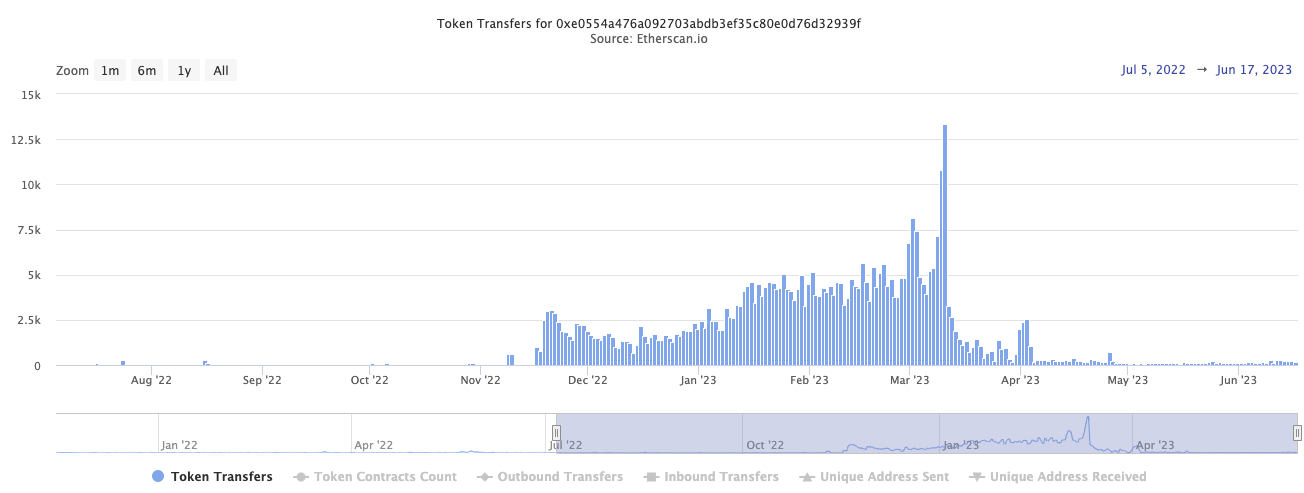
\includegraphics[width=0.8\linewidth]{evaluation/Images/pool-txn-history.png}
    \caption{Number of Token Transfer over time in 0xe0554a476a092703abdb3ef35c80e0d76d32939f~\cite{etherscan-pool}}
    \label{fig:pool-txn-history}
\end{figure}

\section{Evaluation of Strategies}
Overall, given the experiments conducted, the optimal parameters for each strategy are different. Thus, to evaluate each strategy, Table \ref{tab:OptimParams} displays the optimal parameters used for each strategy.

\begin{table}[H]
    \centering
    \begin{tabular}{|p{6em}|p{8em}|p{6em}|p{4em}|p{8em}|}
    \hline
        Strategy & Number of Standard Deviations from the mean, $\#_{\sigma}$ & Gas Price Threshold in ETH & Window Size in Days & Type of Execution, Seperate or Batched \\ \hline
        Constant & 3 & 6.36e-08 & 60 & Batched \\ \hline
        Sliding Window & 2 & 8.83e-08 & 60 & Batched \\ \hline
        Lagged & 2 & 1.29e-07 & 60 & Batched \\ \hline
        Granger Causality & 1.5 & 2.13e-05 & 60 & Batched \\ \hline
        Kalman Filter & 0.5 & 2.13e-05 & 60 & Batched \\ \hline
    \end{tabular}
    \caption{Optimal Parameters for each strategy \label{tab:OptimParams}}
\end{table}

\noindent By running the backtesting system from 14th January 2022 to 9th June 2023 with an initial investment of 100ETH, we can see in Table \ref{tab:FinalResults} the Kalman Filter outperforms all of the other strategies in all liquidity pool pairs except pair 6. The Granger Causality strategy has also performed well. In contrast, the Lagged strategy returned mediocre return, with the Constant and Sliding Window strategies performing similarly, resulting in around 20\% APY.
\\[3mm]
\begin{table}[H]
    \centering
    \begin{adjustwidth}{-0.8in}{-0.9in}
        \begin{tabular}{|p{4em}|p{3em}|p{3em}|p{3em}|p{3em}|p{3em}|p{3em}|p{3em}|p{3em}|p{3em}|p{3em}|}\hline
            Pool Pair & \multicolumn{10}{|c|}{Strategy's Annual Percentage Rate (APR) - Trading from 14th January 2022 to 9th June 2023} \\\cline{2-11}
            & \multicolumn{2}{|c|}{Constant} & \multicolumn{2}{|c|}{Sliding Window} & \multicolumn{2}{|c|}{Lagged} & \multicolumn{2}{|c|}{Granger Causality} & \multicolumn{2}{|c|}{Kalman Filter}\\\cline{2-11}
            & Return \% & \# of Trades & Return \% & \# of Trades & Return \% & \# of Trades & Return \% & \# of Trades & Return \% & \# of Trades\\\hline
            0 & \textcolor{green}{24.84} & 83 & \textcolor{green}{38.61} & 250 & \textcolor{green}{65.5} & 276 & \textcolor{green}{86.91} & 310 & \textcolor{green}{145.74} & 378\\\cline{2-11}
            1 & \textcolor{green}{20.7} & 37 & \textcolor{green}{14.38} & 127 & \textcolor{green}{29.54} & 151 & \textcolor{green}{20.37} & 269 & \textcolor{green}{43.94} & 456\\\cline{2-11}
            2 & \textcolor{green}{22.12} & 46 & \textcolor{green}{30.74} & 103 & \textcolor{green}{49.75} & 112 & \textcolor{green}{92.19} & 218 & \textcolor{green}{164.55} & 396\\\cline{2-11}
            3 & \textcolor{green}{18.14} & 31 & \textcolor{green}{14.26} & 86 & \textcolor{green}{33.67} & 98 & \textcolor{green}{28.51} & 231 & \textcolor{green}{33.36} & 425\\\cline{2-11}
            4 & \textcolor{green}{27.65} & 45 & \textcolor{green}{38.44} & 122 & \textcolor{green}{66.23} & 140 & \textcolor{green}{92.71} & 290 & \textcolor{green}{152.26} & 391\\\cline{2-11}
            5 & \textcolor{green}{23.11} & 25 & \textcolor{green}{25.76} & 77 & \textcolor{green}{45.57} & 98 & \textcolor{green}{31.8} & 299 & \textcolor{green}{57.81} & 388\\\cline{2-11}
            6 & \textcolor{red}{-2.54} & 13 & \textcolor{red}{-10.28} & 30 & \textcolor{red}{-19.31} & 49 & \textcolor{red}{-10.56} & 23 & \textcolor{red}{-29.71} & 150\\\hline\hline           
            Average & \textcolor{green}{19.14} & 40 & \textcolor{green}{21.70} & 113.6 & \textcolor{green}{38.70} & 132 & \textcolor{green}{48.85} & 234.3 & \textcolor{green}{81.14} & 369.1\\\hline                       
        \end{tabular}
    \end{adjustwidth}
    \caption{Returns of each strategy with their optimal parameters \label{tab:FinalResults}}.
\end{table}

\noindent In addition to this, Figure \ref{fig:ValueHistory} shows the account value over time of each of the strategies; it is easy the see that the account values seem to follow a trend; however, the gradients of the return are less drastic in some strategies, i.e. the Kalman Filter. Notably, the number of profitable trades decreased since the beginning of 2023, with the Kalman Filter strategy taking a large loss in January of this year, 2023.

\begin{figure}[H]
    \centering
    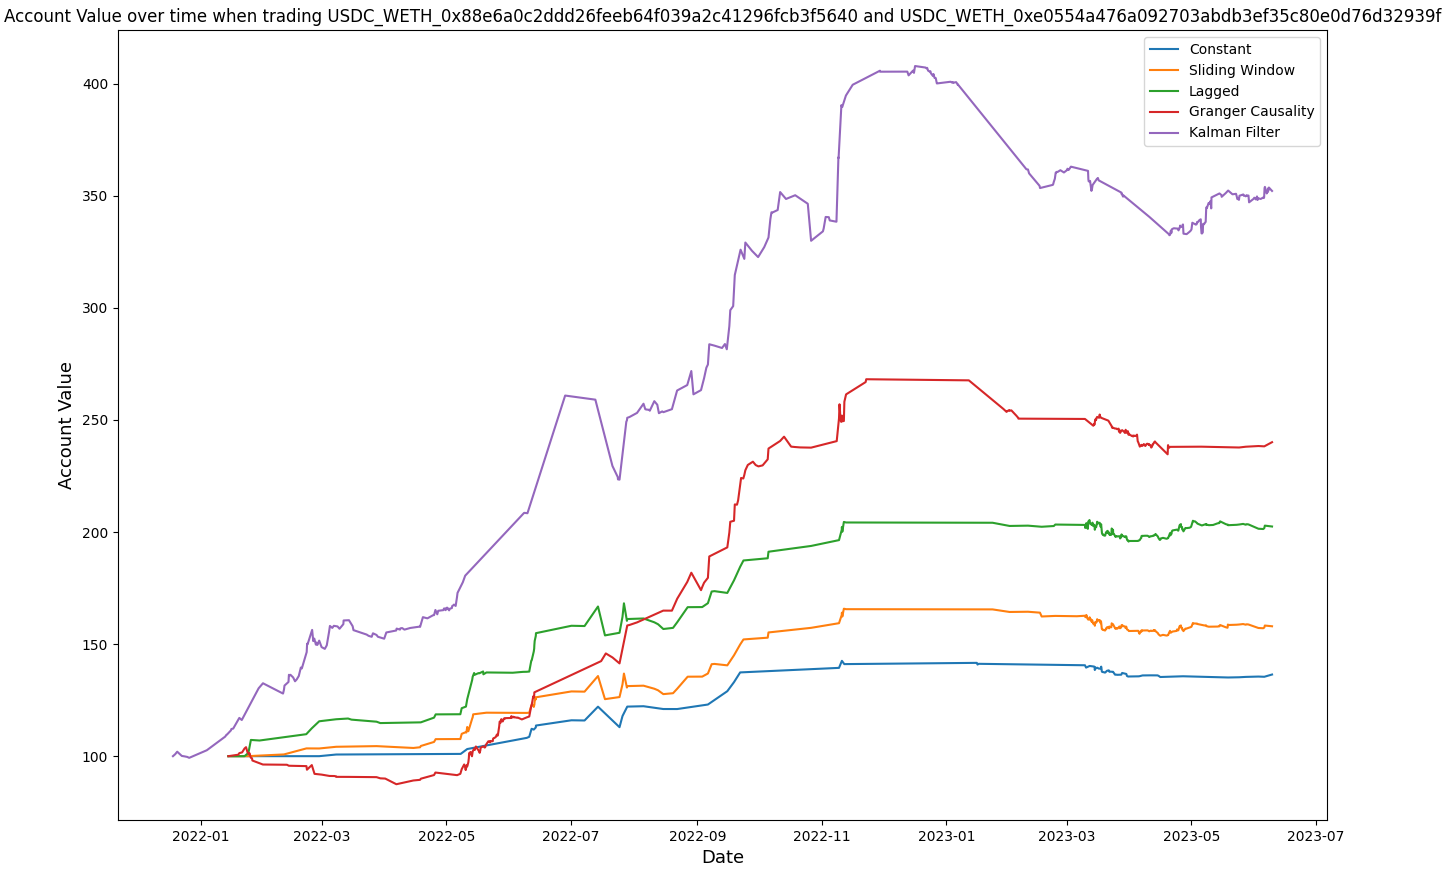
\includegraphics[width=\linewidth]{evaluation/Images/ValueHistory.png}
    \caption{Account Value over Time from backtesting Pair 0}
    \label{fig:ValueHistory}
\end{figure}

\noindent Another valuable insight can be seen in Figure \ref{fig:HedgeRatioPerStrat}, where the evolution of the hedge ratio is plotted for each strategy. It can be seen that the sliding window and the Granger causality strategies' hedge ratios are fairly consistent in comparison to the lagged strategy's hedge ratio. However, the Kalman Filter calculates the Hedge Ratio slightly lower and more constant with only minor deviations, as seen in Figure \ref{fig:evolving_hedge_ratio_kf}. This indicates a more persistent relationship between the paired assets. The minor deviations observed in the hedge ratio can be attributed to temporary fluctuations in market dynamics or noise in the data.

\begin{figure}[H]
    \centering
    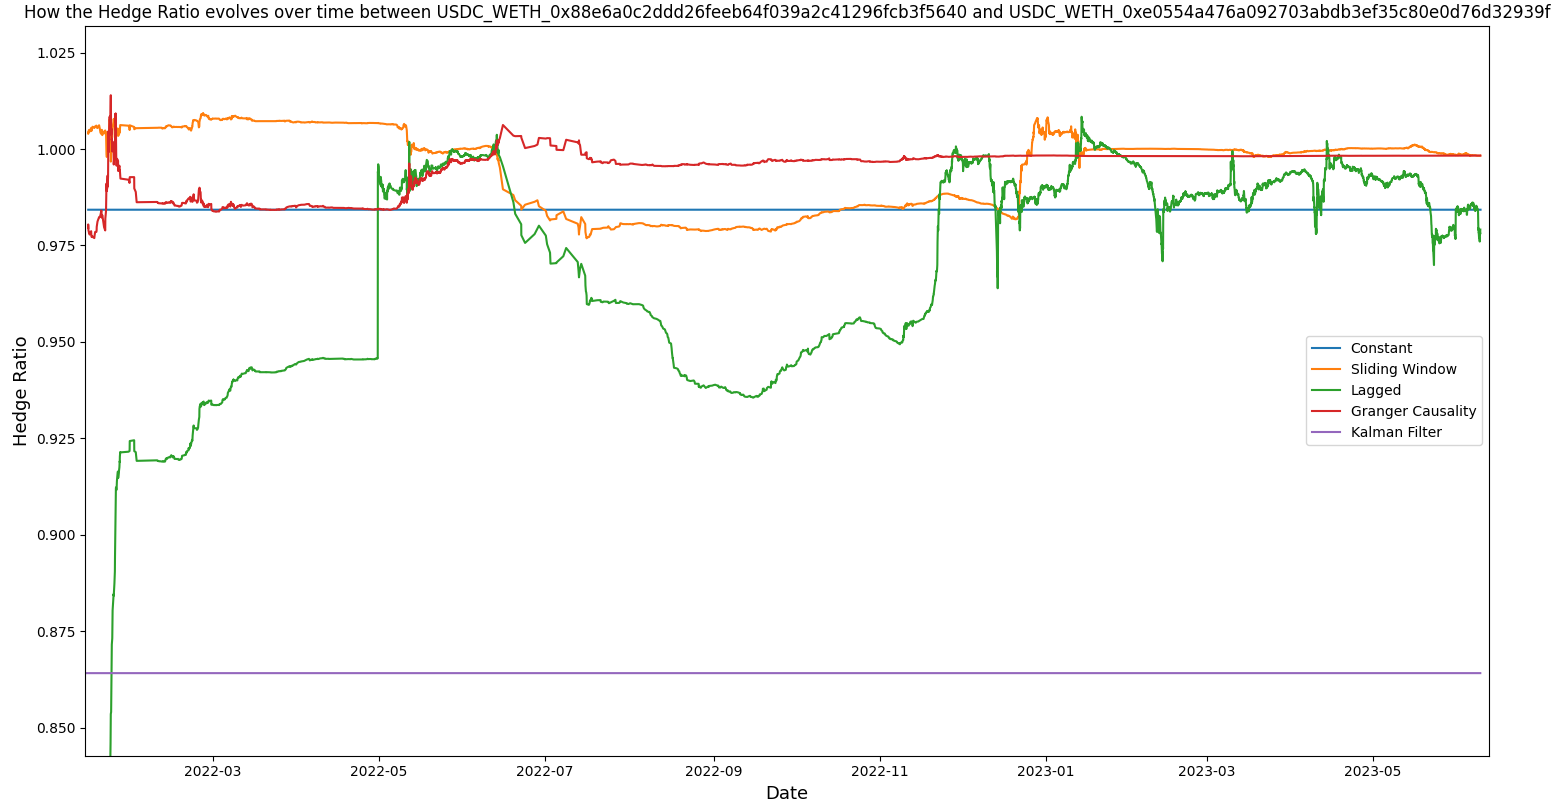
\includegraphics[width=\linewidth]{evaluation/Images/HedgeRatioPerStrat.png}
    \caption{The Hedge Ratio over time for Pair 0}
    \label{fig:HedgeRatioPerStrat}
\end{figure}

\subsection{Beta}
An important metric when evaluating trading strategies or investments used in industry is Beta, $\beta$. It measures how correlated the strategy's return is with the market return rate. It is often used as a risk-reward measure, allowing investors to make better investing decisions, balancing the risk and reward. $\beta$ is defined as $\beta = \frac{Cov(R_M, R_S)}{Var(R_M)}$, where $R_M$ is the market's returns and $R_S$ is the strategy's or stock's returns, the higher the $\beta$ value, the more correlated the strategy's return is with the market. In contrast, in a lower one, i.e. $\rightarrow - \infty$, the strategy swings the opposing direction to the market. Therefore, a low absolute value is ideal in risk-neutral strategies as it minimises the risk.
\\[3mm]
Therefore, to analyse the $\beta$ of each strategy, the conversion from WETH to USD is used as the strategies use WETH as their base currency. As shown in Table \ref{tab:betas}, the $\beta$s are very close to 0, indicating that the strategy's dependence on the market returns is very low. The low $\beta$ values imply that the trading strategy may be designed to generate returns based on factors other than general market movements. It suggests that the strategy relies more on specific signals, indicators, or market inefficiencies rather than broader market conditions. This can be advantageous in certain situations, as it may allow the strategy to perform well even when the overall market is experiencing volatility or downturns.
\\[3mm]
The comparison of account values and the evolution of ETH price over time are depicted in Figure \ref{fig:beta-vis}. The figure illustrates a limited correlation between the trading strategy's returns and ETH's price. While the returns of the strategy do not closely follow the exact movements in the ETH price, it is evident that significant price fluctuations in ETH impact the strategy's performance. This observation suggests that the trading strategy's returns are influenced, to some extent, by the general trends and movements in the price of ETH. However, it is important to note that the relationship is not entirely linear or directly proportional. Therefore, we can conclude that the impact of ETH price changes on the strategy's performance is limited. It can also be seen that the Constant, Sliding Window and Lagged strategies are less affected by the market compared to the Granger Causality and Kalman Filter strategies.

\begin{table}[H]
    \centering
    \begin{adjustwidth}{-0.8in}{-0.9in}
        \begin{tabular}{|p{5em}|p{7em}|p{7em}|p{7em}|p{8em}|p{7em}|}\hline
            Pool Pair & \multicolumn{5}{|c|}{Strategies' Beta, $\beta$ - Trading from 14th January 2022 to 9th June 2023} \\\cline{1-6}
            & Constant & Sliding Window & Lagged & Granger Causality & Kalman Filter\\\cline{2-6}
            0 & -1.57001e-11 & -2.37822e-11 & -2.34107e-11 & -1.17100e-11 & -3.36017e-11\\\cline{2-6}
            1 & -1.33728e-11 & -2.55276e-11 & -2.34361e-11 & -1.48089e-11 & -2.80161e-11\\\cline{2-6}
            2 & -1.44463e-11 & -2.51260e-11 & -2.48695e-11 & -1.08178e-11 & -3.28074e-11\\\cline{2-6}
            3 & -1.30815e-11 & -2.34876e-11 & -2.48109e-11 & -1.12766e-11 & -3.32465e-11\\\cline{2-6}
            4 & -1.38961e-11 & -2.59124e-11 & -2.78297e-11 & -1.86356e-11 & -3.65904e-11\\\cline{2-6}
            5 & -1.43195e-11 & -3.08987e-11 & -2.79315e-11 & -5.46023e-12 & -3.38610e-11\\\cline{2-6}
            6 & 3.42127e-12 & -4.57712e-11 & -3.56508e-11 & -9.80665e-11 & -1.43624e-10\\\hline\hline
            Average & -1.162784e-11 & -2.864367e-11 & -2.684845e-11 & -2.439650e-11 & -4.882103e-11\\\hline
        \end{tabular}
    \end{adjustwidth}
    \caption{$\beta$s of each strategy \label{tab:betas}}.
\end{table}

\begin{figure}[H]
    \centering
    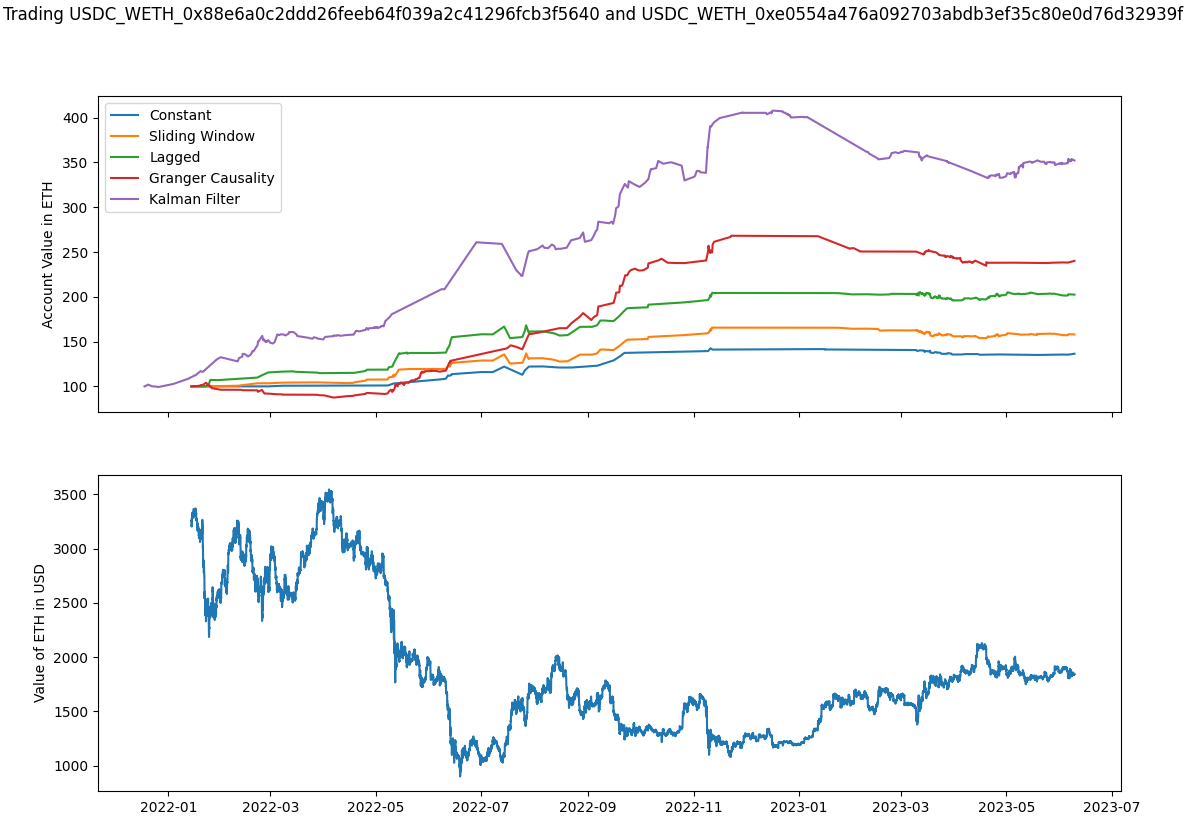
\includegraphics[width=\linewidth]{evaluation/Images/beta_visualisation.png}
    \caption{Account Value of time with the price of ETH}
    \label{fig:beta-vis}
\end{figure}

\subsection{Volatility \& Sharpe Ratio}


Another metric commonly used in finance is the Sharpe Ratio; this is because it is important to evaluate how risky the strategies are compared to the risk-free rate. The metric is given by the formula below:$$\text{Sharpe Ratio} = \frac{R_p - R_f}{\sigma_p}$$ Where $R_p$ is the return of a portfolio, $R_f$ is the risk-free rate and $\sigma_p$ is the standard deviation of the portfolio. A higher Sharpe ratio indicates a better risk-adjusted return, which signifies a higher return than the risk taken. It implies that the investment has achieved a greater excess return compared to the risk-free rate, considering the level of volatility. Conversely, a lower Sharpe ratio suggests a lower risk-adjusted return, indicating a relatively higher level of risk for the given return. The Sharpe ratio also helps investors compare investments or strategies based on risk-adversity performance. It provides a way to assess whether the return generated by an investment adequately compensates for the level of risk taken. 
\\[3mm]
To calculate each of the strategies' Sharpe Ratios, the Bank of England's interest rate of 4.5\%~\cite{boe_interest}. Table \ref{tab:sharpes} displays the Sharpe ratios of each strategy; we see that the Constant Strategy exhibits the highest hedge ratio, followed by the Lagged and Granger Causality strategies, while the Sliding Window and Kalman Filter strategies have the lowest Sharpe ratios. This discrepancy can be attributed to the Kalman Filter strategy having a higher variance, indicating a greater level of risk compared to the Sliding Window, Lagged, and Granger Causality strategies. According to Forbes, a Sharpe ratio $>1$ is considered `good' as it suggests that the investment or strategy has generated a return of more than one unit of risk. Overall, all strategies yield desirable Sharpe ratios, indicating favourable risk-adjusted returns.

\begin{table}[H]
    \centering
        \begin{tabular}{|p{7em}|p{7em}|p{7em}|p{7em}|}\hline
            Strategy & Volatility & Average Return & Sharpe Ratio \\\hline
            Constant & 9.28 & 19.14 & 1.46\\\hline
            Sliding Window & 16.02 & 21.70 & 1.10\\\hline
            Lagged & 27.04 & 38.70 & 1.29 \\\hline
            Granger Causality & 38.35 & 48.85 & 1.20\\\hline
            Kalman Filter & 68.34 & 81.14 & 1.17\\\hline
        \end{tabular}
    \caption{Volatility and Sharpe Ratios of each strategy \label{tab:sharpes}}.
\end{table}

\subsection{Comparison with Previous results}
Overall, the strategies seem to be a desirable investment for those with enough capital; however, how do these investments stand against other techniques? There has not been any research into statistical arbitrage on decentralised exchanges, with the few that have looked into trading in DEXes evaluating pure arbitrage, searching for miss-pricing and executing them. One of which found there to be little to no profitable arbitrage opportunities on various decentralised exchanges, including Uniswap, regardless of volume size~\cite{boonpeam2021arbitrage}. This happens as the pair prices as automatically adjusted based on supply and demand, making the opportunities limited, short-lived and costly. In comparison, the results from the strategies implemented in this paper do generate a profit in comparison to the cyclic arbitrage approach.
\\[3mm]
Other research into statistical approaches to arbitrage has been done on more mainstream assets such as ETFs; however, they have not been experimented on cryptocurrencies. One paper used the Kalman Filter on ETFs and ETNs and found there to be an average of 25.17\% returns in 1 year in in-sample backtesting; however, it failed to generate any profit in its out-of-sample results~\cite{dempsey_market_2017}. The implemented Lagged, Kalman Filter, and Granger Causality trading strategies yield a greater APR than this. In addition to this, another piece of research used a combination of machine learning and the Kalman Filter on assets on the BM\&FBovespa Exchange, yielding a return of 26.13\% in the out-of-sample results~\cite{6974093}. In comparison, the Lagged, Kalman Filter and Granger Causality strategies implemented in this paper have a greater return; however, the strategy implemented by Oliveira and Nóbrega, possesses a greater Sharpe ratio meaning the risk-adjusted returns are more favourable. To summarise, three of the five strategies implemented outperform the current research on both purer forms of arbitrage, i.e. cyclic arbitrage, and the use of Kalman Filter on other types of assets, i.e. ETFs and ETNs.

\chapter{Conclusion}

In conclusion, using the optimal parameters for each of the strategies, the Kalman Filter results in the best return of 81.14\%, Granger Causality with a return of 48.85\%, Lagged has a return of 38.70\% and the Sliding Window and Constant (benchmark) having returns of  21.70\% and 19.14\% respectively. It can be seen that the former strategies perform well above the benchmark, making them appealing to investors. Furthermore, the returns are also not correlated to the market rate furthering its appeal to investors due to its low $|\beta|$ values.
\\[3mm]
Overall, the strategies exhibit strong performance compared to the current state of the art. However, it is important to note that a significant initial investment, approximately 50 ETH equivalent to 86,491.50 USD (based on the conversion rate of $17^{th}$ June 2023), is required to generate a substantial profit. This is primarily due to the transaction costs of executing trades on the Ethereum network. As a result, with higher initial investment, the impact of gas fees becomes relatively insignificant, leading to more profitable outcomes rather than losses. Investors with enough capital would be able to employ these strategies, making the strategies unattractive to the average investor; however, larger institutions may find these strategies appealing with the high return and good Sharpe ratio.

\section{Future Work}

\subsection{Running the Strategies Live}
The next step would be to execute and assess the real-time performance of the trading strategies. By running the strategies live, their effectiveness and profitability can be thoroughly examined, providing valuable insights into their practical application and potential for generating returns.

\subsection{Different Decentralised Exchanges}
To further the research, an intriguing avenue for further exploration would be to assess statistical arbitrage opportunities in other decentralized exchanges (DEXes). By examining the performance of mean reversion strategies across various DEX platforms, valuable insights can be gained regarding the decentralized trading ecosystem and the potential profitability of such trading approaches.

\subsection{Different Tokens}
Furthermore, it is important to acknowledge the limitations of the liquidity pool selection process, specifically regarding the availability of easily borrowable tokens. The current approach relied on tokens readily accessible through Aave, thus imposing a constraint on the pool of eligible tokens. However, as the decentralized ecosystem grows, including additional tokens and lending protocols would facilitate borrowing a wider range of alt-coins, thereby unlocking a multitude of untapped arbitrage possibilities.

\subsection{Different Blockchains}
The Ethereum blockchain was chosen as the primary focus of this project due to its extensive ecosystem and diverse functionalities. However, with the rise in popularity of various other blockchains for different reasons, it becomes intriguing to explore the performance of the same trading strategies when applied to different blockchain networks. Evaluating the returns from running the strategies on alternative blockchains can provide valuable insights into the comparative profitability and potential opportunities across different blockchain ecosystems.

\appendix
\chapter{Additional Background}
\section{Pure Arbitrage}
\label{appendix:add-background-pure-arb}
As mentioned in Chapter \ref{sec:pure-arb}, research into this topic is still in its infancy thus which means a very thin slice of exploration on the subject matter. The majority of the research has been into the arbitrage on centralised exchanges~\cite{MakarovIgor2020Taai, crepelliere_arbitrage_2022, PAUNACristian2018ATSf}. Cristian Pauna investigates and implements an arbitrage strategy in~\cite{PAUNACristian2018ATSf}. The paper details the technical details of arbitrage trading from the data and the system architecture used. Pauna finds complications such as requesting data from multiple exchanges, converting the data such that it is homogeneous and also managing server load. Pauna presents the architecture such that the servers request data from the necessary exchanges, aggregating prices in a relational database which then triggers a server that is used to generate trading signals.
\\[3mm]
\begin{figure}[!htb]
    \centering
    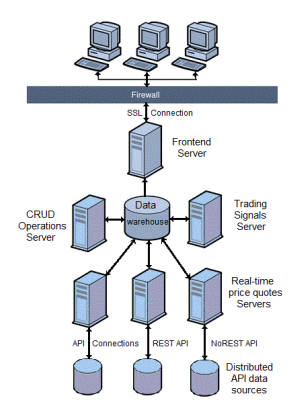
\includegraphics[width=0.28\textwidth]{background/Images/Arbitrage-Architecture.png}
    \caption{Arbitrage system architecture~\cite{PAUNACristian2018ATSf}}
\end{figure}

\noindent Triangular and cyclic arbitrage is one of the most used and purest forms of arbitrage to implement and analyse,~\cite{boonpeam2021arbitrage} explores triangular arbitrage on decentralised exchanges. Algorithm \ref{alg:arb_sys_on_dex} is the algorithm used to find the most profitable arbitrage route on a particular platform, once this is calculated, it is compared with other routes on other platforms. Initially, the system converts the base token into another token and converts it back into the base token, using only one token is used as a middle route, then using the algorithm below, increases the number of middle tokens.
\\[3mm]

\begin{algorithm}
    \caption{Maximum Profit Route Searching (R)}\label{alg:arb_sys_on_dex}
    \textbf{Input}: $T$ (token list), $P$ (price graph), $n$ (current route)
    \begin{algorithmic}
        \For{$i = 1, ..., T$}
        \State $r = get\_profit(n+i)$
        \For{$j = 1,...,P[i]$}
        \State $p = max(r, R(T, P, n_j))$
        \EndFor
        \EndFor
        \State \textbf{return} $p$
    \end{algorithmic}
\end{algorithm}

\noindent On evaluating the performance of the strategy on differing platforms depended on three main features of each exchange:
\begin{enumerate}
    \item Portion size - Depending on how much the ``trader'' invested revenues differed and with the larger portion size, the revenue decreases as the token pair prices are adjusted based on supply/demand.
    \item Transaction fees - Each exchange has its own transaction fee.
    \item Other considerations such as price slippage - Exchanges have different liquidity levels which depend on the usage and liquidity providers that the exchange employs.
\end{enumerate}

\noindent Figure \ref{fig:arb_on_diff_exchanges} displays the revenues obtained by same trading token route, ETH $\rightarrow$ MKR $\rightarrow$ OMG $\rightarrow$ USDT $\rightarrow$ ETH. As we can see upon applying the strategy on multiple exchanges; Uniswap, 1inch, Kyberswap and Bancor, 1 inch was the only exchange that generated a profit whereas the others lose money~\cite{boonpeam2021arbitrage}. 
\\[3mm]
\begin{figure}[!htb]
    \centering
    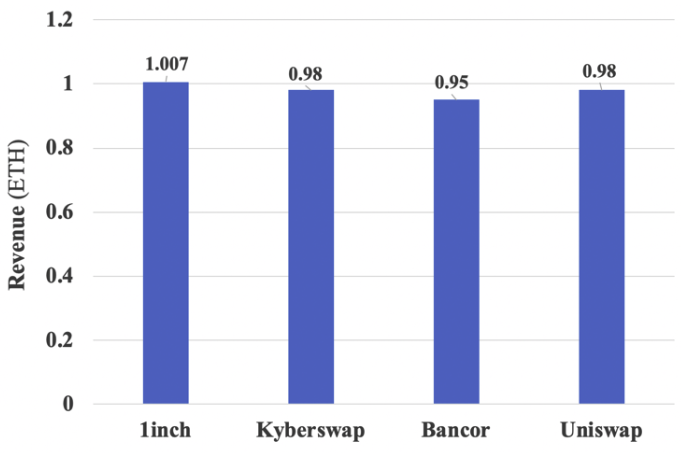
\includegraphics[width=0.6\textwidth]{background/Images/revenue_oncyclic_arb.png}
    \caption{Trading profits same token routes within different exchanges~\cite{boonpeam2021arbitrage} \label{fig:arb_on_diff_exchanges}}
\end{figure}

\noindent Another paper that implemented and evaluated a cyclic arbitrage opportunity is~\cite{wang_cyclic_2022}. The research consists of proposing a theoretical arbitrage model and further evaluation of real transactional data. The arbitrage model used is simple to understand, as it searches for a cyclic transaction between $n$ tokens, $A_1, A_2, ..., A_n$ is a sequence of $n$ trades:
\begin{center}
    \begin{minipage}[c]{0.4\linewidth}
        \begin{itemize}
            \item[\textit{Trade 1:}] Exchange $\delta_1$ of $A_1$ to $\delta_2$ of $A_2$
            \item[\textit{Trade 2:}] Exchange $\delta_2$ of $A_2$ to $\delta_3$ of $A_3$
            \item[] $\dotsc$
            \item[\textit{Trade n:}] Exchange $\delta_n$ of $A_n$ to $\delta_1'$ of $A_1$
        \end{itemize}
    \end{minipage}
\end{center}

\noindent It is important to note that $\delta_i = \delta_{i+1}$, i.e. the output of trade is equivalent to the input of the next. The revenues within a cycle are defined as $\delta_{i+1} - \delta_i$, and the overall profit is $\delta_{1}' - \delta_1$. This is not as simple as the revenues depend on how liquid the exchange is, thus the liquidity pools of each possible trading pair are hugely important. Therefore, the paper proposes a theorem, below:

\begin{theorem}
    For a given cycle $A_1 \rightarrow A_2 \rightarrow \cdots \rightarrow A_n \rightarrow A_1$ with $n$ tokens, there exists an arbitrage opportunity for the cyclic transaction if the product of exchange rates $\frac{a_{2,1}a_{3,2}\cdots a_{1,n}}{a_{1,2}a_{2,3}\cdots a_{n, 1}} > \frac{1}{r_1^n r_2^n}$ where $a_{i,j}$ denotes the liquidity of token $A_i$ in the liquidity pool with token $A_j$.~\cite{wang_cyclic_2022}
\end{theorem}

\noindent In addition to the theorem, to obtain an optimal strategy we need to compute the optimal trading volume of a cycle, $A_1 \rightarrow A_2 \rightarrow \cdots \rightarrow A_n \rightarrow A_1$. The paper proposes the optimal trading volume to be $\delta^{op}_a = \frac{\sqrt{r_1 r_2 a' a} - a}{r_1}$ where $a = \frac{a_{1,n}'a_{n,1}}{a_{n,1}+r_1 r_2 a_{n,1}'}$ and $a' = \frac{r_1 r_2 a_{1,n}'a_{n,1}}{a_{n,1}+r_1 r_2 a_{n,1}'}$. Thus to calculate such arbitrage opportunities knowing the liquidity of tokens in other tokens' liquidity pools, algorithm \ref{alg:liquidity_alg} infers the direction and volumes to trade to get the optimal revenue.

\begin{algorithm}
    \caption{Computing the equivalent liquidity of the cycle}\label{alg:liquidity_alg}
    \begin{algorithmic}
        \State $a_{1, n}' \leftarrow a_{1,2}$
        \State $a_{n, 1}' \leftarrow a_{2,1}$
        \For{$i$ from $2$ to $n-1$}
        \State $a_{1, n}' \leftarrow \frac{a_{1,n}'a_{i,i+1}}{a_{i,i+1}+r_1 r_2 a_{n,1}'}$
        \State $a_{n, 1}' \leftarrow \frac{r_1 r_2 a_{1,n}'a_{i+1, i}}{a_{i,i+1}+r_1 r_2 a_{n,1}'}$
        \EndFor
    \end{algorithmic}
\end{algorithm}

\noindent After analyzing Ethereum block data and applying this strategy to identify the number of arbitrage opportunities, it was found that between May 4, 2020, and April 15, 2021, there were numerous exploitable and profitable arbitrage opportunities. These opportunities grew consistently to reach 1,750 in 11 months, as depicted in Figure \ref{fig:exploitable_ops}. Only cycles with length 3 were experimented with and only cycles including ETH as 80\% of the liquidity pools on Uniswap include ETH and another cryptocurrency~\cite{heimbach2021behavior}. Furthermore, it is found that 287,241 of the 292,606 arbitrages executed started with ETH, and 85\% of the arbitrages used a cycle of length 3. The total revenue of the cyclic arbitrage was 34,429 ETH. However, gas fees account for 24.6\% of the total revenue leaving an approximate 25,971 ETH profit.
\\[3mm]
\begin{figure}[!htb]
    \centering
    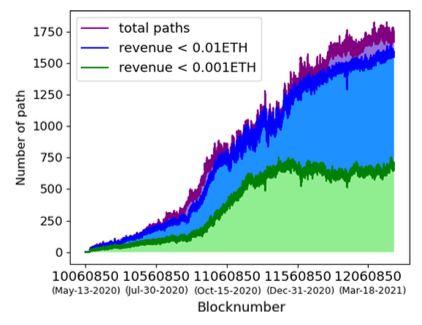
\includegraphics[width=0.6\textwidth]{background/Images/exploitable_ops.png}
    \caption{Number of exploitable opportunities in Uniswap V2 over time. The purple line represents the number of cycles that provide revenue higher than 0.0001 ETH. The green represents the number of cycles whose revenue is under 0.001 ETH. The blue line represents the number of cycles whose revenue is under 0.01 ETH.~\cite{wang_cyclic_2022} \label{fig:exploitable_ops}}
\end{figure}

\noindent The paper then delves into the implementation of the smart contract, and explores how both \textit{sequential} and \textit{atomic} implementations would affect the revenue and execution of the contracts. It was found that 52.3\% of the arbitrages that were executed sequentially generated a loss, likely due to the fact that, when one submits $n$ orders, the $n$ blockchain transactions are executed sequentially, meaning some external transactions can be inserted between these transactions. Thus using atomic transactions avoids this issue of external transactions does not affect the market price that may affect the outcome of the arbitrage.
\\[3mm]
Furthermore, the authors of the paper also investigated the performance differences between using private smart contracts and public contracts. Deploying a smart contract that calls Uniswap functions, i.e. a private smart contract, is intuitively better and achieves a higher success rate of a lower bound of 52\% and a higher bound of 90\% in comparison to calling a public Uniswap smart contract which has a success rate of 27.3\%. Overall the paper provides an insightful look into cyclic arbitrage in DEXes and highlights important decisions made such as liquidity calculations and smart contracts while comparing the performance of different options available.

\section{Optimal Portfolio Design for Mean Reversion}
\label{appendix:add-background-opt-portfolio-des-mean-revers}
There has been further research into optimizing mean reversion, one of which was to use the successive convex approximation method on the mean reverting portfolio design ~\cite{ZipingZhao2019OMPW}. The paper initially proposes the mean reversion portfolio:
\begin{itemize}
    \itemsep0em
    \item For each asset, the price at time $t$ is denoted as $p_t$ and its correspondeing log-price $y_t \triangleq log(p_t)$, its vector form of $M$ assets $\mathbf{y}_t \triangleq \big[ y_{1,t}, \dots ,y_{M,t} \big]^T$.
    \item The log-price spread is given by $y_t \triangleq \mathbf{\beta}^T\mathbf{y}_t$, where $\mathbf{\beta} \triangleq \big[ \beta_1, \dots ,\beta_M \big]^T$ denotes the hedge ratios.
    \item The cointegration space with $N$ relations is defined by $\mathbf{B} \triangleq \big[ \beta_1, \dots ,\beta_N \big]$, thus the $N$ spreads are $s_t \triangleq \mathbf{B}^T\mathbf{y}_t$.
    \item For these $N$ spreads, the portfolio weight matrix is denoted as $\mathbf{w} \triangleq \big[ w_1, \dots ,w_N \big]^T$.
    \item The auto-covariance matrix for the spreads $s_t$ is defined as \\ ${M_i \triangleq Cov(s_t, s_{t+i}) = \mathop{\mathbb{E}} \big[ \big( s_t - \mathop{\mathbb{E}} \big[ s_t \big]\big) \big( s_{t+i} - \mathop{\mathbb{E}} \big[ s_{t+i} \big]\big)^T \big]}$
\end{itemize}

\noindent Now that we have defined everything required, we can now formalize the problem. The general problem of mean reversion portfolio design problem is formalized by:
\begin{equation*}
    \begin{aligned}
         & \underset{\mathbf{w}}{\text{minimize}}
         &                                        & F(\mathbf{w}) \triangleq U(\mathbf{w}) + \mu V(\mathbf{w}) + \gamma S(\mathbf{w})                                                                       \\
         & \text{subject to}
         &                                        & \mathbf{w} \in \biggl\{ \mathbf{w} \mid \big\| \mathbf{B} \mathbf{w}\big\|_0 \leq L \biggr\}, \qquad \text{where $L$ is the total leveraged investment}
    \end{aligned}
\end{equation*}

\begin{itemize}
    \item $\mu$ defines the trade-off between the mean reversion measure and the variance preference.
    \item $\gamma$ defines the regularization parameter of how sparse we would like the cointegration space to be.
\end{itemize}

\noindent Where the Mean Reversion term: $$U(\mathbf{w}) \triangleq \xi \frac{\mathbf{w}^T \mathbf{H}\mathbf{w}}{\mathbf{w}^T \mathbf{M}_0\mathbf{w}} + \zeta \biggl( \frac{\mathbf{w}^T \mathbf{M}_1\mathbf{w}}{\mathbf{w}^T \mathbf{M}_0\mathbf{w}} \biggr) ^2 + \eta \sum_{i=2}^{p} \biggl( \frac{\mathbf{w}^T \mathbf{M}_i\mathbf{w}}{\mathbf{w}^T \mathbf{M}_0\mathbf{w}}\biggr)^2$$ And the variance term: $$V(\mathbf{w}) \triangleq \begin{cases}
        1/\mathbf{w}^T \mathbf{M}_0\mathbf{w}        & \text{VarInv(\textbf{w})} \\
        1/\sqrt{\mathbf{w}^T \mathbf{M}_0\mathbf{w}} & \text{StdInv(\textbf{w})} \\
        -\mathbf{w}^T \mathbf{M}_0\mathbf{w}         & \text{VarNeg(\textbf{w})} \\
        -\sqrt{\mathbf{w}^T \mathbf{M}_0\mathbf{w}}  & \text{StdNeg(\textbf{w})}
    \end{cases}$$
The variance term can be represented in any of the four forms.
\\[3mm]
And the asset selection term: $$S(\mathbf{w}) \triangleq \big\| \mathbf{B} \mathbf{w}\big\|_0 = \sum_{m=1}^{M} sgn(\mid \bigl[ \mathbf{B} \mathbf{w} \bigr]_m \mid)$$ This asset selection criterion is not necessary however as trading incurs a cost, selecting all of the assets is costly, thus selecting a subset of assets to trade is more profitable. To formalize this goal, we would like to minimize the cointegration space thus we use the $\ell_0$ norm.
\\[3mm]
The paper then goes on to solve the optimization problem using the successive convex approximation (SCA) method~\cite{scaOptimization}. The SCA method takes an optimization problem in the form of:
\begin{equation*}
    \begin{aligned}
         & \underset{\mathbf{x}}{\text{minimize}}
         &                                        & f(\mathbf{x})              \\
         & \text{subject to}
         &                                        & \mathbf{x} \in \mathcal{X}
    \end{aligned}
\end{equation*}
\noindent Where $\mathcal{X} \subseteq \mathbb{R}^N$ is convex and $f(\mathbf{x})$ is non-convex. The SCA method involves starting at an initial point $\mathbf{x}^{(0)}$ and solving a series of subproblems of surrogate funtions $\tilde{f}(\mathbf{x}; \mathbf{x}^{(k)})$ over the set $\mathcal{X}$. The sequence $\bigl\{ \mathbf{x}^{(k)} \bigr\}$ is generated by: $$\begin{cases}
        \hat{\mathbf{x}}^{(k+1)} = arg \underset{\mathbf{x} \in \mathcal{X}}{min} \tilde{f}(\mathbf{x}; \mathbf{x}^{(k)}) \\
        \mathbf{x}^{(k+1)} = \mathbf{x}^{(k)} + \gamma^{(k)}(\hat{\mathbf{x}}^{(k+1)} - \mathbf{x}^{(k)})
    \end{cases}$$
The first step is to generate a descent direction and then update the variable with a step size of $\gamma^{(k)}$. After applying this method to the MRP problem and further analysis of the paper, the following algorithm is proposed and used to solve the MRP design problem:
\begin{algorithm}
    \caption{SCA-Based Algorithm for The Optimal MRP Design Problem}\label{alg:sca_alg}
    \textbf{Require}: $\mathbf{H}, \mathbf{M}_i, \mu, \gamma, \mathbf{B}, L \text{ and } \tau$
    \begin{algorithmic}[1]
        \State Set $k=0, \gamma^{(0)}$ and $\mathbf{w}^{(0)}$
        \Repeat
        \State Compute $\mathbf{A}^{(k)}$ and $\mathbf{b}^{(k)}$
        \State $\hat{\mathbf{w}}^{(k+1)} = arg \underset{\mathbf{w} \in \mathcal{W}}{min} \mathbf{w}^{T}\mathbf{A}^{(k)}\mathbf{w} + \mathbf{b}^{(k)T}\mathbf{w}$
        \State $\mathbf{w}^{(k+1)} = \mathbf{w}^{(k)} + \gamma^{(k)}(\hat{\mathbf{w}}^{(k+1)} - \mathbf{w}^{(k)})$
        \State $k \leftarrow k+1$
        \Until convergence
    \end{algorithmic}
\end{algorithm}

\noindent However, 4 line is a convex problem and has no closed-form solution thus to solve this subproblem using the ADMM method, this is done by introducing an auxiliary variable $\mathbf{z = Bw}$.
\begin{equation*}
    \begin{aligned}
         & \underset{\mathbf{x, z}}{\text{minimize}}
         &                                           & \mathbf{w}^{T}\mathbf{A}\mathbf{w} + \mathbf{b}^{T}\mathbf{w} \\
         & \text{subject to}
         &                                           & \big\| \mathbf{z} \big\|_1 \leq B, \mathbf{Bw - z=0}
    \end{aligned}
\end{equation*}
\noindent This is then summarized into Algorithm \ref{alg:admm_alg}:
\begin{algorithm}
    \caption{An ADMM-Based Algorithm for Problem on line 4 in Algorithm \ref{alg:sca_alg}}\label{alg:admm_alg}
    \textbf{Require}: $\mathbf{A}, \mathbf{b}, \mathbf{B}, B, \rho$
    \begin{algorithmic}[1]
        \State Set $\mathbf{w}^{(0)}, \mathbf{z}^{(0)}, \mathbf{u}^{(0)}$ and $k=0$
        \Repeat
        \State $\mathbf{w}^{(k+1)} = -(2\mathbf{A} + \rho \mathbf{B}^T\mathbf{B})^{-1}(\mathbf{b} + \rho \mathbf{B}^T(\mathbf{u}^{(k)} - \mathbf{z}^{(k)}))$
        \State $\mathbf{h}^{(k)} = \mathbf{Bw}^{(k+1)} + \mathbf{u}^{(k)}$
        \State $\mathbf{z}^{(k+1)} = \Pi_{\mathcal{C}}(\mathbf{h}^{(k)})$
        \State $\mathbf{u}^{(k+1)} = \mathbf{u}^{(k)} + \mathbf{Bw}^{(k+1)} - \mathbf{z}^{(k+1)}$
        \State $k \leftarrow k+1$
        \Until convergence
    \end{algorithmic}
\end{algorithm}

\noindent After all of this analysis, the authors of the paper, \cite{8450775, ZipingZhao2019OMPW}, ran simulations on real data comparing underlying spread. It found that it resulted in consistent profits as shown in Figure \ref{fig:ROIsMRP}.
\\[3mm]
\begin{figure}[htb!]
    \centering
    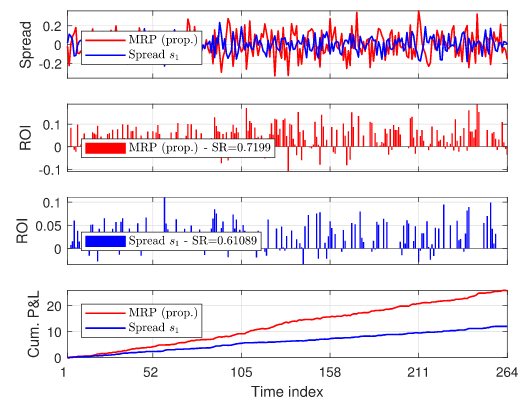
\includegraphics[width=0.4\textwidth]{background/Images/rois1.png}
    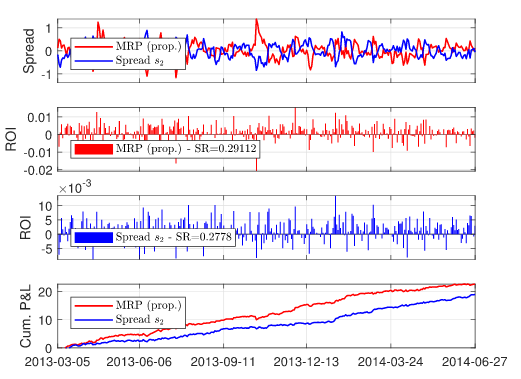
\includegraphics[width=0.43\textwidth]{background/Images/rois2.png}
    \caption{A mean-reversion trading based on real data~\cite{ZipingZhao2019OMPW}}
    \label{fig:ROIsMRP}
\end{figure}

\noindent Overall, this research successfully formulizes, solves the optimization problem mathematically, and goes further to implement the algorithms to solve the problem programmatically. In addition, the author compares the implementation with other benchmark algorithms, showing that it results in a greater P\&L and Sharpe ratio.

\chapter{Supporting Tables}
\section{Exerpt of the liquidity\_pools Table}
\begin{table}[!ht]
    \centering
    \begin{tabular}{|p{7em}|p{4em}|p{4em}|p{10em}|p{\linewidth / 6}|p{4em}|}
    \hline
        pool address & token0 & token1 & volume in USD & created at timestamp & feetier \\ \hline
        \truncate{7em}{0x88e6a0c2ddd26feeb64f039a2c41296fcb3f5640} & USDC & WETH & \truncate{10em}{375230561243.465} & 1620250931 & 500 \\ \hline
        \truncate{7em}{0x8ad599c3a0ff1de082011efddc58f1908eb6e6d8} & USDC & WETH & \truncate{10em}{70454095868.0967} & 1620169800 & 3000 \\ \hline
        \truncate{7em}{0x11b815efb8f581194ae79006d24e0d814b7697f6} & WETH & USDT & \truncate{10em}{62385006691.8387} & 1620251172 & 500 \\ \hline
        \truncate{7em}{0x3416cf6c708da44db2624d63ea0aaef7113527c6} & USDC & USDT & \truncate{10em}{57192593471.8346} & 1636825557 & 100 \\ \hline
        \truncate{7em}{0x4585fe77225b41b697c938b018e2ac67ac5a20c0} & WBTC & WETH & \truncate{10em}{49170385539.9928} & 1620246230 & 500 \\ \hline
        \truncate{7em}{0x4e68ccd3e89f51c3074ca5072bbac773960dfa36} & WETH & USDT & \truncate{10em}{30135014933.0963} & 1620232628 & 3000 \\ \hline
        \truncate{7em}{0x60594a405d53811d3bc4766596efd80fd545a270} & DAI & WETH & \truncate{10em}{26075053939.434} & 1620237823 & 500 \\ \hline
        \truncate{7em}{0xcbcdf9626bc03e24f779434178a73a0b4bad62ed} & WBTC & WETH & \truncate{10em}{21870989841.1326} & 1620158974 & 3000 \\ \hline
        \truncate{7em}{0x5777d92f208679db4b9778590fa3cab3ac9e2168} & DAI & USDC & \truncate{10em}{16143305036.8948} & 1636771503 & 100 \\ \hline
        \truncate{7em}{0x7858e59e0c01ea06df3af3d20ac7b0003275d4bf} & USDC & USDT & \truncate{10em}{15473402409.0591} & 1620159478 & 500 \\ \hline
        \truncate{7em}{0x99ac8ca7087fa4a2a1fb6357269965a2014abc35} & WBTC & USDC & \truncate{10em}{12568187132.1649} & 1620241995 & 3000 \\ \hline
        \truncate{7em}{0xc2e9f25be6257c210d7adf0d4cd6e3e881ba25f8} & DAI & WETH & \truncate{10em}{12519316091.9979} & 1620159368 & 3000 \\ \hline
        \truncate{7em}{0xe0554a476a092703abdb3ef35c80e0d76d32939f} & USDC & WETH & \truncate{10em}{9381529300.20357} & 1636926269 & 100 \\ \hline
        \truncate{7em}{0x6c6bc977e13df9b0de53b251522280bb72383700} & DAI & USDC & \truncate{10em}{7219493916.70291} & 1620158293 & 500 \\ \hline
        \truncate{7em}{0xac4b3dacb91461209ae9d41ec517c2b9cb1b7daf} & APE & WETH & \truncate{10em}{6621032721.87519} & 1647516735 & 3000 \\ \hline
        \truncate{7em}{0x8c54aa2a32a779e6f6fbea568ad85a19e0109c26} & FEI & USDC & \truncate{10em}{6206853090.73714} & 1621839430 & 500 \\ \hline\hline
        \truncate{7em}{0x53dd58b3143f428b449c16dd5706cee7d7bcf408} & sOHM & gOHM & 0 & 1652914688 & 10000 \\ \hline
        \truncate{7em}{0xbc90c4de85a4b559060cb28abfd4476ab6711f1a} & SHIB & NSTIC & 0 & 1652910391 & 100 \\ \hline
        \truncate{7em}{0xaa1297b08d0035f06309c1bfa36582c24b4ae361} & BUSD & DPC & 0 & 1674655715 & 100 \\ \hline
        \truncate{7em}{0x75087e5330c97f7ec7f716c6566f214cb0029f6a} & DAI & ICAP & 0 & 1652899566 & 10000 \\ \hline
        \truncate{7em}{0xc65a680191bd17a18c957c8aa2d1155ed2322792} & stkAAVE & FRAX & 0 & 1652817927 & 10000 \\ \hline
        \truncate{7em}{0x94589b18b95b355ee9a900f3df671b431779e20a} & VVV & SOL & 0 & 1674701603 & 10000 \\ \hline
        \truncate{7em}{0xf42f0def92337b6a83753c9fae6d579f7d67aaa9} & APEFI & ApeUSD & 0 & 1652808878 & 3000 \\ \hline
        \truncate{7em}{0xb9ba65f1568b318ffc1879a4a6368ef2b5ac96b8} & FRAX & ApeUSD & 0 & 1652808680 & 500 \\ \hline
        \truncate{7em}{0x1dfb167f1ba47f3bf835eb60a9317b4601925642} & GHD & WETH & 0 & 1652784327 & 3000 \\ \hline
    \end{tabular}
    \caption{A selection of liquidity pools on Uniswap \label{tab:liquidity_pools}}
\end{table}

\chapter{Supporting Algorithms}

\section{Gas Price Collection}
\begin{algorithm}
    \caption{Retrieval of hourly gas prices where $min\_time$ \& $max\_time$ are arguments}\label{alg_gas_price_col}
    \begin{algorithmic}
        \State $rows\_set \leftarrow \{\}$
        \For{$timestamp$ from $min\_time$ to $max\_time + (60 \times 60), step\_size = (60 \times 60)$}
            \State $found\_result \leftarrow False$
            \State $window\_size\_in\_minutes \leftarrow 5$
            \While{$not\ found\_result$}
                \State $transaction\_data \leftarrow$ GraphQL Query with arguments: $\{``min\_time": timestamp - (60 * window\_size\_in\_minutes), ``max\_time": timestamp + (60 * window\_size\_in\_minutes)\}$
                \If{$transaction\_data != 0$}
                    \State $transaction\_data\_sorted = sorted(transaction\_data, key=lambda\ x:abs(timestamp - int(x['timestamp'])))$
                    \State $rows\_set.update({timestamp: (timestamp, transaction\_data\_sorted[0]['gasPrice'])})$
                    \State $found\_result \leftarrow True$
                \Else
                    \State $window\_size\_in\_minutes \leftarrow window\_size\_in\_minutes + 5$
                \EndIf
            \EndWhile
            \State insert $rows\_set[timestamp]$ into \texttt{gas\_prices} table
        \EndFor
    \end{algorithmic}
\end{algorithm}

\chapter{Supporting Code Snippets}

\section{Data Collection GraphQL Queries}

\subsection{Uniswap Pool Historical Price Data Collection}

\begin{lstlisting}[caption={GraphQL query to collect for pool pricing data \label{app:pool-query}},captionpos=b]
query ($id: ID!, $prev_max_time: Int!) {
    pool(id: $id) {
        poolHourData(where: {periodStartUnix_gt: $prev_max_time}, orderBy: periodStartUnix, first: 1000) {
            id
            token0Price
            token1Price
            periodStartUnix
            liquidity
            feesUSD
        }
    }
}
\end{lstlisting}

\subsection{Uniswap Pool Live Price Data Collection \label{app:live-pool-price-query}}
\begin{lstlisting}[caption={GraphQL query to collect for live pricing data },captionpos=b]
query ($id: ID!) {
    pool(id: $id) {
        token0 {
            symbol
        }
        token1 {
            symbol
        }
        token0Price
        token1Price
        liquidity
    }
}
\end{lstlisting}

\subsection{Uniswap Historical Gas Price Data Collection}
\begin{lstlisting}[caption={GraphQL query to collect for gas pricing data \label{app:gas-query}},captionpos=b]
query ($min_time: Int!, $max_time: Int!) {
    transactions(where: {timestamp_gt: $min_time, timestamp_lt: $max_time}, first:1000, orderBy: timestamp, orderDirection: asc) {
        id
        timestamp
        gasPrice
    }
}
\end{lstlisting}

\subsection{Uniswap Live Gas Price Data Collection\label{app:live-gas-query}}
\begin{lstlisting}[caption={GraphQL query to collect for live gas price data},captionpos=b]
query {
    transactions(first:1, orderBy: timestamp, orderDirection:desc) {
        gasPrice
        timestamp
    }
}
\end{lstlisting}


\subsection{Aave Historical Lending Pool Data Collection \label{app:lending-query}}
\begin{lstlisting}[caption={GraphQL query to retrieve for lending pricing data},captionpos=b]
query ($symbol: String!, $prev_max_time: Int!) {
    reserves(where: {symbol: $symbol}) {
        id
        symbol
        lifetimeBorrows
        baseLTVasCollateral
        reserveLiquidationThreshold
        borrowHistory(
            where: {timestamp_gt: $prev_max_time}, first: 1000, orderBy: timestamp, orderDirection: asc) {
            id
            timestamp
            borrowRate
        }
    }
}
\end{lstlisting}

\section{Backtesting Code Snippets}

\subsection{Order Execution Code}
\label{sec:backtesting-execution-code}

\subsubsection{Buying ETH}
\begin{lstlisting}[language=Python, caption={Execution code for Buying ETH},captionpos=b]
amount_to_swap = self.account['WETH'] * order[1]
self.account['WETH'] = self.account['WETH'] - amount_to_swap
self.account['ETH'] = self.account['ETH'] + amount_to_swap
\end{lstlisting}

\subsubsection{Swapping Tokens}
\begin{lstlisting}[language=Python, caption={Execution code for Swapping Tokens on a specified liquidity pool},captionpos=b]
if is_for_token0:
    for swap_for_token0 in swaps:
        swap_token, swap_volume = swap_for_token0
        self.account['WETH'] = self.account['WETH'] - (swap_volume * prices[f'P{swap_token[1]}'])
        self.account[swap_token] = self.account[swap_token] + (swap_volume * (1 - swap_fees[swap_token]))
else:
    for swap_for_token1 in swaps:
        swap_token, swap_volume = swap_for_token1
        self.account[swap_token] = self.account[swap_token] - (swap_volume / prices[f'P{swap_token[1]}'])
        self.account['WETH'] = self.account['WETH'] + (swap_volume * (1 - swap_fees[swap_token]))
\end{lstlisting}

\subsubsection{Opening a Buy Position}
\begin{lstlisting}[language=Python, caption={Execution code for opening a buy positon},captionpos=b]
self.account['WETH'] = self.account['WETH'] - (volume * buy_price)
self.account[token] = self.account[token] + (volume * (1 - swap_fees[token]))
\end{lstlisting}

\subsubsection{Closing a Buy Position}
\begin{lstlisting}[language=Python, caption={Execution code for closing a buy positon},captionpos=b]
buy_token, bought_price, buy_volume, buy_timestamp = self.open_positions['BUY'][buy_id]
volume_bought = buy_volume * (1 - swap_fees[buy_token])
self.account[buy_token] = self.account[buy_token] - volume_bought
self.account['WETH'] = self.account['WETH'] + (prices[f'P{buy_token[1]}'] * (volume_bought * (1 - swap_fees[buy_token])))
\end{lstlisting}


\subsubsection{Opening a Sell Position}
\begin{lstlisting}[language=Python, caption={Execution code for opening a sell positon},captionpos=b]
# Borrow token and Deposit collateral
amount_to_move_to_collateral_WETH = ((volume * sell_price) / ltv_eth)
self.account[token] = self.account[token] + volume
self.account['WETH'] = self.account['WETH'] - amount_to_move_to_collateral_WETH
self.account['collateral_WETH'] = self.account['collateral_WETH'] + amount_to_move_to_collateral_WETH

# Swap borrowed tokens to WETH
self.account[token] = self.account[token] - volume
self.account['WETH'] = self.account['WETH'] + (volume * (1 - swap_fees[token]) * sell_price)
\end{lstlisting}


\subsubsection{Closing a Sell Position}
\begin{lstlisting}[language=Python, caption={Execution code for closing a sell positon},captionpos=b]
sell_token, sold_price, sell_volume, sell_timestamp = self.open_positions['SELL'][sell_id]

# Swap WETH back to Token
volume_required_to_return = sell_volume
previous_timestamp = sell_timestamp

for apy_idx in apy[sell_token].index:
    local_apy = apy[sell_token].loc[apy_idx]['borrow_rate']
    number_of_seconds = apy[sell_token].loc[apy_idx]['timestamp'] - previous_timestamp
    secondly_yield = (1 + local_apy)**(1 / (365*24*60*60))
    volume_required_to_return *= secondly_yield ** number_of_seconds
    previous_timestamp = apy[sell_token].loc[apy_idx]['timestamp']

self.account['WETH'] = self.account['WETH'] - (sold_price * volume_required_to_return / (1 - swap_fees[sell_token])) 
self.account[sell_token] = self.account[sell_token] + volume_required_to_return

# Return Borrowed Tokens and Collatoral
self.account[sell_token] = self.account[sell_token] - volume_required_to_return
self.account['WETH'] = self.account['WETH'] + self.account['collateral_WETH']
self.account['collateral_WETH'] = 0
\end{lstlisting}

\subsubsection{Withdrawing Collatoral}
\begin{lstlisting}[language=Python, caption={Execution code for withdrawing a selected amount of collateral},captionpos=b]
self.account['WETH'] = self.account['WETH'] + withdraw_amount
self.account['collateral_WETH'] = self.account['collateral_WETH'] - withdraw_amount
\end{lstlisting}

\subsubsection{Depositing Additional Collatoral}
\begin{lstlisting}[language=Python, caption={Execution code for depositing a selected amount of collateral},captionpos=b]
self.account['WETH'] = self.account['WETH'] - deposit_amount
self.account['collateral_WETH'] = self.account['collateral_WETH'] + deposit_amount
\end{lstlisting}

\subsubsection{Deducting Gas Fees on \texttt{OPEN} and \texttt{CLOSE} Orders \label{app:deducting-gas-fee}}
\begin{lstlisting}[language=Python, caption={Execution code for deducting gas fees on \texttt{OPEN} and \texttt{CLOSE} orders},captionpos=b]
if len([order[0] for order in signal if order[0] == 'OPEN']) == 2:
    if strategy.should_batch_trade:
        self.account['ETH'] = self.account['ETH'] - (GAS_USED_BY_OPEN_BUY_AND_SELL_POSITION * gas_price_in_eth)
    else:
        self.account['ETH'] = self.account['ETH'] - ((GAS_USED_BY_SWAP + GAS_USED_BY_SWAP + GAS_USED_BY_BORROW) * gas_price_in_eth)

if len([order[0] for order in signal if order[0] == 'CLOSE']) == 2:
    if strategy.should_batch_trade:
        self.account['ETH'] = self.account['ETH'] - (GAS_USED_BY_CLOSE_BUY_AND_SELL_POSITION * gas_price_in_eth)
    else:
        self.account['ETH'] = self.account['ETH'] - ((GAS_USED_BY_SWAP + GAS_USED_BY_SWAP + GAS_USED_BY_REPAY) * gas_price_in_eth)

\end{lstlisting}


\subsection{Strategy Hedge Ratio Calculation Code \label{app:strats-hr-calcs}}

\subsubsection{Constant Strategy}
\begin{lstlisting}[language=Python, caption={Calculation of the hedge ratio of the Constant Strategy},captionpos=b]
model = sm.OLS(history_p1, sm.add_constant(history_p2))
results = model.fit()
# Gradient of the OLS i.e. X = results.params[0] + results.params[1] * 'p2_token1_price'
hedge_ratio = params[1]
\end{lstlisting}

\subsubsection{Sliding Window Strategy}
\begin{lstlisting}[language=Python, caption={Calculation of the hedge ratio in \texttt{update\_hedge\_ratio} of the Sliding Window Strategy},captionpos=b]
def update_hedge_ratio(self):
    p1, p2 = self.history_p1[-window_size:], self.history_p2[-window_size:]
    model = sm.OLS(p2, sm.add_constant(p1))
    results = model.fit()
    self.hedge_ratio = results.params[1]
\end{lstlisting}

\subsubsection{Lagged Strategy}
\begin{lstlisting}[language=Python, caption={Calculation of the hedge ratio in \texttt{update\_hedge\_ratio} of the Lagged Strategy},captionpos=b]
def update_hedge_ratio(self):
    maxlag = min(self.lag, min(self.window_size_in_hours, len(self.history_p1))-1)
    p1, p2 = self.history_p1[-(self.window_size_in_hours+maxlag):], self.history_p2[-self.window_size_in_hours:]
    lagged_p1 = sm.tsa.lagmat(p1, maxlag=maxlag)[-self.window_size_in_hours:]
    model = sm.OLS(p2, sm.add_constant(lagged_p1))
    results = model.fit()
    self.hedge_ratio = results.params[1]
\end{lstlisting}

\subsubsection{Granger Causality Test Strategy}
\begin{lstlisting}[language=Python, caption={Calculation of the hedge ratio in \texttt{update\_hedge\_ratio} of the Granger Causality Test Strategy},captionpos=b]
def update_hedge_ratio(self):
    p1, p2 = self.history_p1, self.history_p2
    data = pd.DataFrame({'Asset1': p1, 'Asset2': p2})
    granger_results = statsmodels.tsa.stattools.grangercausalitytests(data, maxlag=[1], verbose=False)
    self.hedge_ratio = granger_results[1][1][1].params[0]
\end{lstlisting}


\subsubsection{Kalman Filter Strategy}
\begin{lstlisting}[language=Python, caption={Calculation of the hedge ratio in \texttt{update\_hedge\_ratio} of the Kalman Filter Strategy},captionpos=b]
def update_hedge_ratio(self):
    x, y = self.history_p2[-1], self.history_p1[-1]
    state_means_stepwise, state_covs_stepwise = self.kf.filter_update(
        filtered_state_mean=self.means_trace[-1],
        filtered_state_covariance=self.covs_trace[-1],
        observation=x,
        observation_matrix=np.array([[y, 1]]))

    self.means_trace.append(state_means_stepwise)
    self.covs_trace.append(state_covs_stepwise)
\end{lstlisting}


\bibliographystyle{IEEEtran}
\bibliography{bibs/sample}
\addcontentsline{toc}{chapter}{References}

\end{document}